\documentclass[10pt]{article}

\usepackage[top=0.79in, bottom=0.79in, left=1in, right=1in]{geometry}

\setlength{\textwidth}{6in}

\usepackage{graphicx}
\graphicspath{/dos/My Documents/My LaTeX Documents/Wave Optics}

\usepackage{amsmath}

\begin{document}
\begin{center}
\Large \textbf{Wave optics}
\end{center}

\begin{center}
These notes are based on lectures by David Binks in The University of Manchester given in Feb-May 2010. Please note, that this is full set of lecture notes as given by Dr Binks "word by word". Almost all pictures and diagrams are from original Dr Binks' slides. Main equations are boxed.
\end{center}
\newpage

\tableofcontents
\newpage

\section{Introduction}
\subsection{Introductory remarks}
In Optics we are interested in time average of all quantities.

Optics -- study of electromagnetic waves, when 

\begin{itemize}
\item[(i)] in vacuum or dielectric (air or gas) there are no charges and currents;
\item[(ii)] at very high frequences.
\end{itemize}

So we determine conditions under which wave-like behaviour is seen.

\subsection{Maxwell's equations}
Maxwell's equations in free space:
\begin{equation}\boxed{
\begin{gathered}
\nabla \vec{E} = 0 \\
\nabla \vec{B} = 0 \\
\nabla \times \vec{B} = \epsilon\epsilon_0 \mu\mu_0 \frac{\partial \vec{E}}{\partial t} \\
\nabla \times \vec{E} = - \frac{\partial \vec{B}}{\partial t} \\
\end{gathered}
}\end{equation}
for a dielectric $\epsilon\neq 1$, $\mu\approx 1$
\begin{equation}
\boxed{\nabla^2 \vec{E} = \epsilon\epsilon_0 \mu_0 \frac{\partial^2 \vec{E}}{\partial t^2}}
\end{equation}
this is an equation for a wave travelling with velocity
\begin{equation*}
v=\frac{1}{\sqrt{\epsilon\epsilon_0 \mu_0}} = \frac{c}{\sqrt{\epsilon}} = \frac{c}{n}
\end{equation*}

In free space:
\begin{equation*}
v=c
\end{equation*}
\begin{equation*}
n=1
\end{equation*}

\subsection*{Properties of EM waves}
\begin{equation}
\boxed{c\vec{B} = \hat{k} \times \vec{E}}
\end{equation}
$\hat{k}$ -- propagation vector.

This implies that electromagnetic waves are \textsl{transverse, orthogonal and in phase}.

Every flux density or energy crossing unit area per second is given by \textit{Poynting vector}.

\begin{equation}
\boxed{\vec{S}=\frac{1}{\mu_0}[\vec{E} \times \vec{B}]}
\end{equation}
$\hat{S}$ is the direction of energy flux.
\begin{equation*}
|\vec{S}| = \frac{E^2}{\eta_0}
\end{equation*}
where
\begin{equation*}
\eta_0 = \sqrt{\frac{\mu_0}{\epsilon_0}}
\end{equation*}
which is known as plane wave impedance and has a value of $377\Omega$.

$|\vec{S}|$ is also an intensity, so intesity is not equal to $E^2$, but is proportional to it.

We generally abserve the time-averaged flux, which is called irradiance or intensity.
\begin{equation*}
I = \langle S \rangle_T
\end{equation*}
where
\begin{equation*}
\langle f(t) \rangle_T = \frac{1}{T} \int^{t+\frac{\pi}{2}} _{t-\frac{\pi}{2}} f(t')dt'
\end{equation*}
$T$ -- averaging interval.
\begin{equation*}
I = \frac{\langle E^2 \rangle_T}{\eta_0}
\end{equation*}

From EM:
\begin{equation*}
\vec{E}(\vec{r},t) = \vec{E_0}\cos(\vec{k}\vec{r} - \omega t)
\end{equation*}
\begin{equation*}
\langle E^2 \rangle_T = \frac{E_0 ^2}{2}
\end{equation*}
\begin{equation}
\boxed{I = \frac{E_0 ^2}{2 \eta_0}}
\end{equation}
because it is mathematically convinient we use
\begin{equation*}
\vec{E}(\vec{r},t) = \vec{E_0} e^{i(kz - \omega t)}
\end{equation*}
where only $\Re{(E)}$ has physical significance. But in this case
\begin{equation*}
\langle E^2 \rangle_T = \langle EE^{*} \rangle_T = E_0 ^2
\end{equation*}
so we have to remember about the factor of $\frac{1}{2}$ -- take real part \underline{before} doing time-average.

\subsection{General solution to wave equation}
\begin{equation*}
v^2 \nabla^2 \vec{E} = \frac{\partial \vec{E}}{\partial t}
\end{equation*}
this is second order PDE with four independent variables -- three space and one time.

Use separation of variables technique.
Let
\begin{equation*}
\vec{E}(\vec{r},t) = \vec{E_r}(\vec{r})E_t(t)
\end{equation*}
\textbf{N.B.:} $E_t$ may be a vector but then $E_r$ must be a scalar.

Substitute in wave equation.
\begin{equation*}
v^2 \nabla^2(E_r E_t) = \frac{\partial^2}{\partial t^2}(E_r E_t)
\end{equation*}
\begin{equation*}
E_t v^2 \nabla^2 E_r = E_r \frac{\partial^2 E_t}{\partial t^2}
\end{equation*}
\begin{equation}
\boxed{\frac{1}{E_r}v^2 \nabla^2 E_r = \frac{1}{E} \frac{\partial^2 E_t}{\partial t^2}}
\end{equation}
this is only truth when both sides are equal to constant.

\subsubsection{Variation with time}
Consider RHS:
\begin{equation*}
\frac{1}{E_t} \frac{\partial^2 E_t}{\partial t^2} = -\omega^2
\end{equation*}
since we are expecting the oscillating solution:
\begin{equation}
\boxed{E_t = E_0 e^{\pm \omega t}}
\end{equation}

Let $E_0 = 1$, then amplitude information is containing in $E_r$. $\omega$ is oscillation frequency.
\begin{equation*}
\omega = 2 \pi\nu
\end{equation*}
\textbf{N.B.:} Linear contributions of $\sin{\omega t} + \cos{\omega t}$ are also solutions, representing physical quantity, but we will use $e^{\pm \omega t}$ for convenience.

\subsubsection{Variation in space}
LHS is:
\begin{equation*}
\nabla^2 \vec{E_r} = - \frac{\omega^2}{v^2}\vec{E_r}^2
\end{equation*}
\begin{equation*}
\frac{\omega^2}{v^2} = k^2
\end{equation*}
\begin{equation}\boxed{
\nabla^2 \vec{E_r} = -k^2 \vec{E_r}
}\end{equation}
this is sometimes called Helmholtz equation.
\begin{equation*}
k = \frac{n \omega}{c} = \frac{n2\pi}{\lambda}
\end{equation*}
$\vec{k}$ -- propagation vector. $k=|\vec{k}|$ -- wave number. \\
\textbf{N.B.:} Wave number is sometimes defined as
\begin{equation*}
k = \frac{1}{\lambda} = \frac{\nu}{c}
\end{equation*}

Helmholtz equation has many solutions which depend on symmetry and bound by conditions.

Full solution is
\begin{equation*}
\vec{E}(\vec{r},t) = \vec{E_0}(\vec{r})e^{\pm i\omega t}
\end{equation*}
in future can write
\begin{equation*}
\vec{E}(\vec{r},t) = \vec{E}(\vec{r})e^{\pm i\omega t}
\end{equation*}

\subsection{Particular solution of wave equation}
\begin{enumerate}
\item Plane waves
\begin{itemize}
\item[$\to$] distant sources;
\item[$\to$] parallel rays;
\item[$\to$] spatial frequencies;
\item[$\to$] Fourier optics;
\item[$\to$] Fraunhofer diffraction;
\end{itemize}
\item Spherical waves
\begin{itemize}
\item[$\to$] Huygens wavelets;
\item[$\to$] Huygens-Frensel principle;
\item[$\to$] Frensel diffraction;
\item[$\to$] focused light;
\item[$\to$] new sources;
\end{itemize}
\item Cylindrical waves
\begin{itemize}
\item[$\to$] $(1) + (2)$;
\item[$\to$] Young's slits;
\item[$\to$] diffraction from a slit.
\end{itemize}
\end{enumerate}

\subsubsection{Plane waves}
Separate $x,y,z$ components, i.e. when
\begin{equation*}
E(\vec{r}) = E_xE_yE_z
\end{equation*}
Substitute into Helmholtz equation:
\begin{equation*}
\vec{E} = \left(
\begin{tabular}{c}
$E_x$ \\
$E_y$ \\
$E_z$ \\
\end{tabular} \right)
\end{equation*}
\begin{equation*}
\frac{1}{E_x} \frac{\partial^2 E_x}{\partial x^2} + \frac{1}{E_y} \frac{\partial^2 E_y}{\partial y^2}  + \frac{1}{E_z} \frac{\partial^2 E_z}{\partial z^2}= -k^2
\end{equation*}
\begin{equation*}
-(k_x ^2 + k_y ^ 2 + k_z ^2) = -k^2
\end{equation*}
\begin{equation*}
\frac{1}{E_x} \frac{\partial^2 E_x}{\partial x^2} = -k_x ^2
\end{equation*}
and so on.
\begin{equation*}
E = E_0 e^{\pm i(k_x x + k_y y + k_z z)} = E_0 e^{\pm i\vec{k} \vec{r}}
\end{equation*}

Full situation:
\begin{equation}\boxed{
E = E_0 e^{\pm i\vec{k} \vec{r} \pm \omega t}
}\end{equation}

\subsubsection{Wavefronts}
Wavefront is a surface of a constant phase.

For a plane wave $\vec{k}\vec{r} \pm \omega t = const$. This defines wavefront.

At particular time fixed (frozen) $\vec{k} \vec{r} = const$. That defines a plane.

That is why we treat this solution as plane wave solution.
\subsubsection*{Wavefront velocity.}
\begin{equation*}
\phi = \vec{k}\vec{r} \pm \omega t
\end{equation*}
\begin{equation*}
\frac{\partial \phi}{\partial t} = \vec{k}\vec{\dot{r}} \pm \omega = 0
\end{equation*}
since wavefront is constant.
\begin{equation*}
\frac{dr}{dt} = \mp \frac{\omega}{\vec{k}} = \mp v_p
\end{equation*}
velocity in $\vec{k}$-direction.
\begin{itemize}
\item $E_0 e^{i(kr-\omega t)}$ -- travelled in $\vec{k}$ direction;
\item $E_0 e^{i(kr + \omega t)}$ -- travelled in $-\vec{k}$ direction
\end{itemize}
at velocity $v_p$.

\subsubsection{Spherical waves}
Consider a point source from which light spreads out (or converges to) isotropically.
\begin{equation}\boxed{
E(\vec{r}) = E(r)
}\end{equation}

For spherical symmetry
\begin{equation*}
\nabla^2 E = \frac{1}{r} \frac{\partial^2}{\partial r^2}(rE) = -k^2 E
\end{equation*}
\begin{equation*}
\frac{\partial^2}{\partial r^2}(rE) = -k^2(rE)
\end{equation*}
regarding $rE$ as a variable
\begin{equation*}
rE = A e^{\pm ikr}
\end{equation*}
\begin{equation}\boxed{
E = A \frac{1}{r}e^{\pm ikr}
}\end{equation}
\textbf{N.B.:} $I \sim EE^* \Rightarrow I \sim \frac{1}{r^2}$

Full solution:
\begin{equation*}
E = A \frac{1}{r}e^{i(kr \pm \omega t)}
\end{equation*}

Constant phase surface -- wavefront
\begin{equation*}
\phi_0 = kr \pm \omega t
\end{equation*}
front phase
\begin{equation*}
0 = k\frac{dr}{dt} \pm \omega
\end{equation*}
\begin{equation*}
\frac{dr}{dt} = \mp \frac{\omega}{k} = \mp v_p
\end{equation*}

The solution $\frac{1}{r}e^{i(kr - \omega t)}$ is diverging light, and $\frac{1}{r}e^{i(kr + \omega t)}$ is converging light.

\subsection{Optical spectra}
\begin{equation*}
E = E_0 e^{i(kr - \omega t}
\end{equation*}
\begin{itemize}
\item $kr$ -- spatial frequency,
\item $\omega t$ -- angular frequency
\end{itemize}
for a plane wave.
\subsubsection{Frequency spectrum}
\begin{equation}\boxed{
E = E_0 e^{-i\omega t}
}\end{equation}
is a solution of $\omega E$.

Therefore is any linear combination
\begin{equation*}
E = \sum_{n=0} ^\infty A_n e^{-i\omega t}
\end{equation*}

If $\omega$ varies continuosly, we can define
\begin{equation}\boxed{
E(t) = \int_{-\infty} ^\infty A_\omega(\omega)e^{-i\omega t}d\omega
}\end{equation}
that's an inverse Fourier transform, where
\begin{equation}\boxed{
A_\omega(\omega) = \frac{1}{2\pi}\int_{-\infty} ^{\infty} E(t)e^{i\omega t}dt
}\end{equation}

So the spectra of light is just a Fourier transform of time-dependent part of electric field. $A_\omega(\omega)$ -- spectrum.

\subsubsection{Spatial frequencies}
Similarily,
\begin{equation}\boxed{
E(x)=\int_{-\infty} ^\infty A_k(k)e^{ikx}dk
}\end{equation}
\begin{equation}\boxed{
A_k = \frac{1}{2\pi}\int_{-\infty} ^\infty E(x) e^{-ikx}dx
}\end{equation}
that's for forward going wave solution. $k$ are the spatial frequencies.\\
\textbf{Note:} restricted to propagation along $x$ to keep it $1D$, and therefore to form simple case of FT.

Any spatial distribution of light can be constructed from a superposition of plane waves.

Note, that in general, $k$ is a vector, so spatial spectrum can consist of plane waves with different $\lambda$ orientations.

\subsection{Principles of propagation}
\begin{itemize}
\item[I] Huygens wavelets.\\
Every point in a wavefront acts as a source of secondary wavelets (with same $\nu$, $v_p$, etc). These wavelets destructively interfere in all but one directions to form new wavefront.
\item[II] Fermat principle -- the principle of the least time.\\
Light takes minimal time to travel between two points, i.e. minimal optical path length
\begin{equation}
\boxed{L = \sum_{i=1}^N n_il_i}
\end{equation}
that takes into account phase resfraction coused by high $n$.
\end{itemize}

\section{Geometric Optics}
\subsection{Introductory remarks}
Optical field is represented by rays.

Ray is a normal to the wavefront.
\begin{figure}[h!]
\begin{minipage}[b]{0.5\linewidth}
\centering
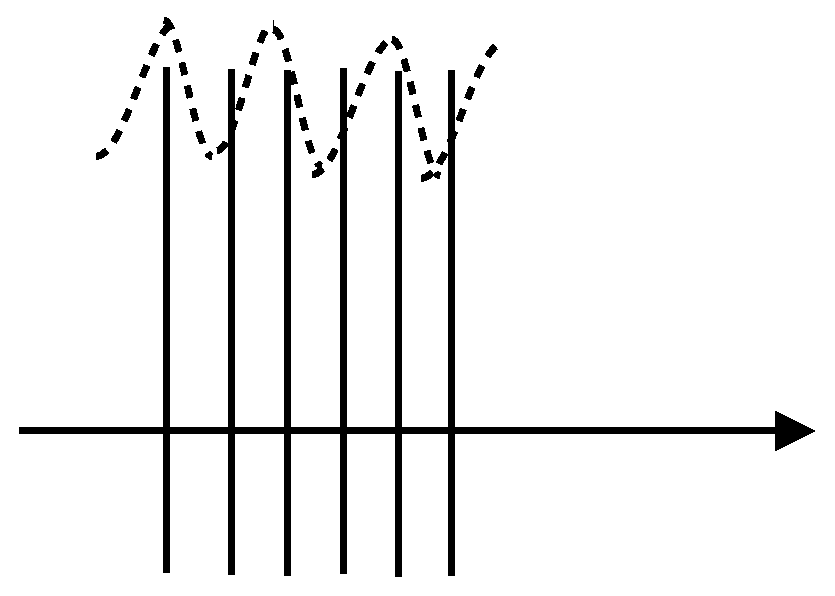
\includegraphics[scale=0.5]{Rays1.eps}
\vspace{0.75cm}
\end{minipage}
\hspace{0.5cm}
\begin{minipage}[b]{0.5\linewidth}
\centering
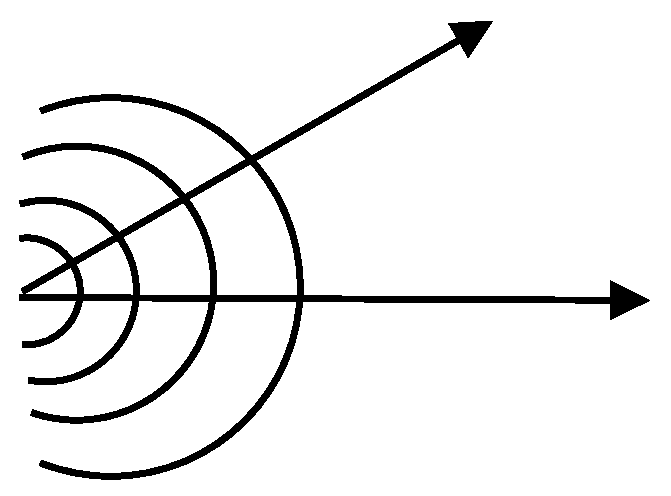
\includegraphics[scale=0.5]{Rays2.eps}
\vspace{0.75cm}
\end{minipage}
\end{figure}

In general rays are parallel to $\vec{S}$.

Rays can be used when interference and diffraction are negligible when wavelength is small comparing to the objects in system.

\subsection{Reflection and Refraction}
By geometry we can easily prove Snell's law using optical path length and Fermat's principle.
\begin{figure}
\centering
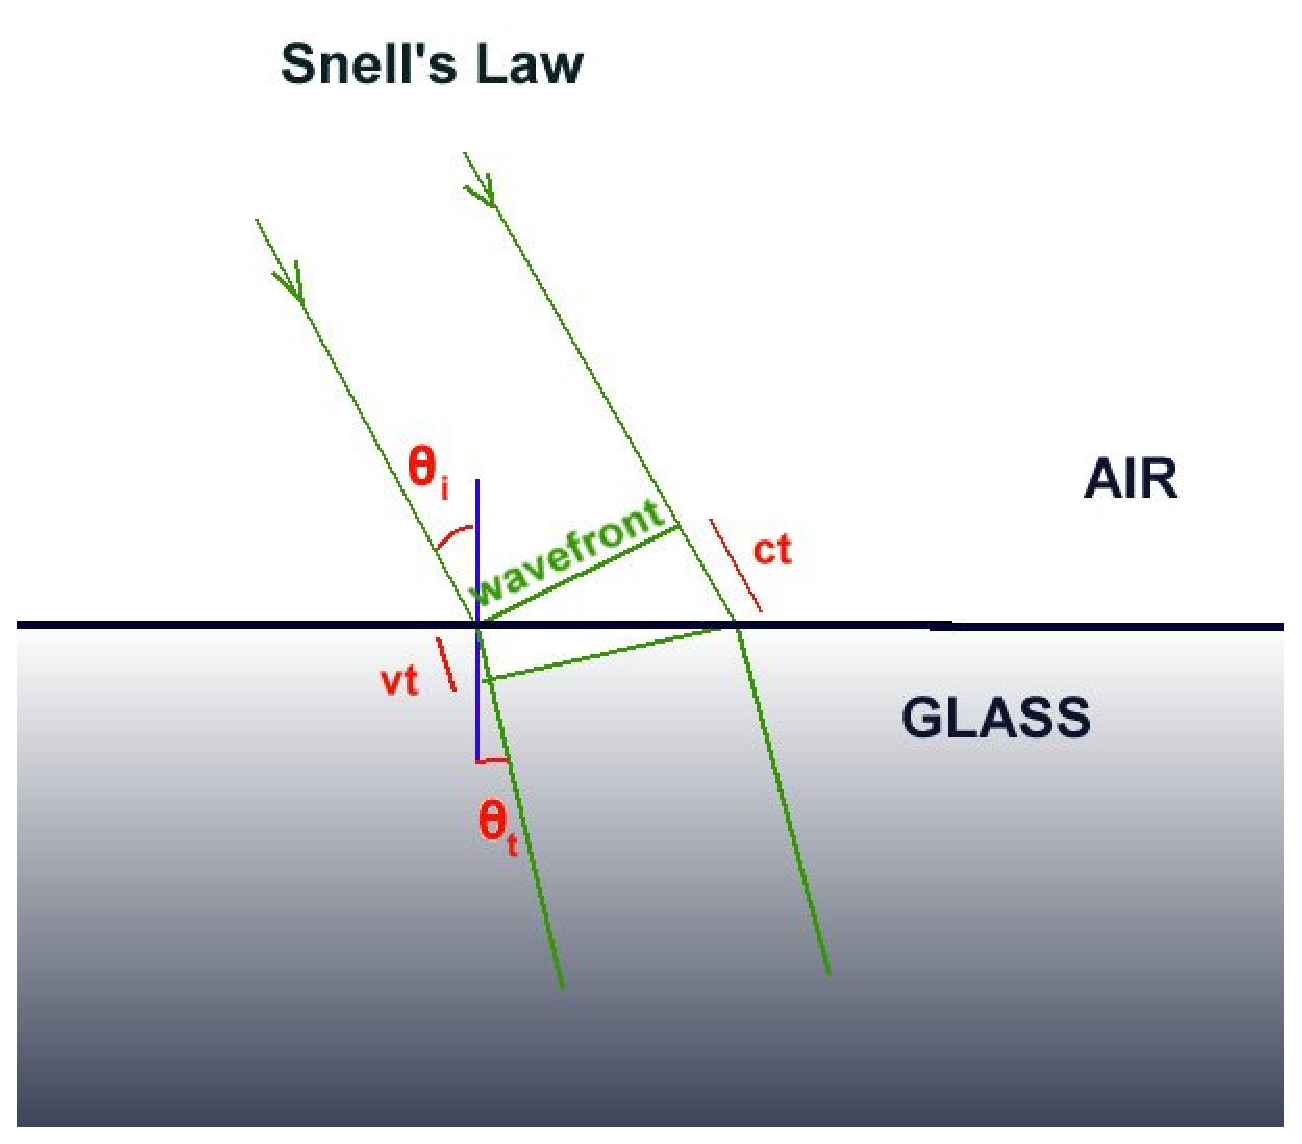
\includegraphics[scale=0.25]{image-0.eps}
\end{figure}
\begin{figure}
\centering
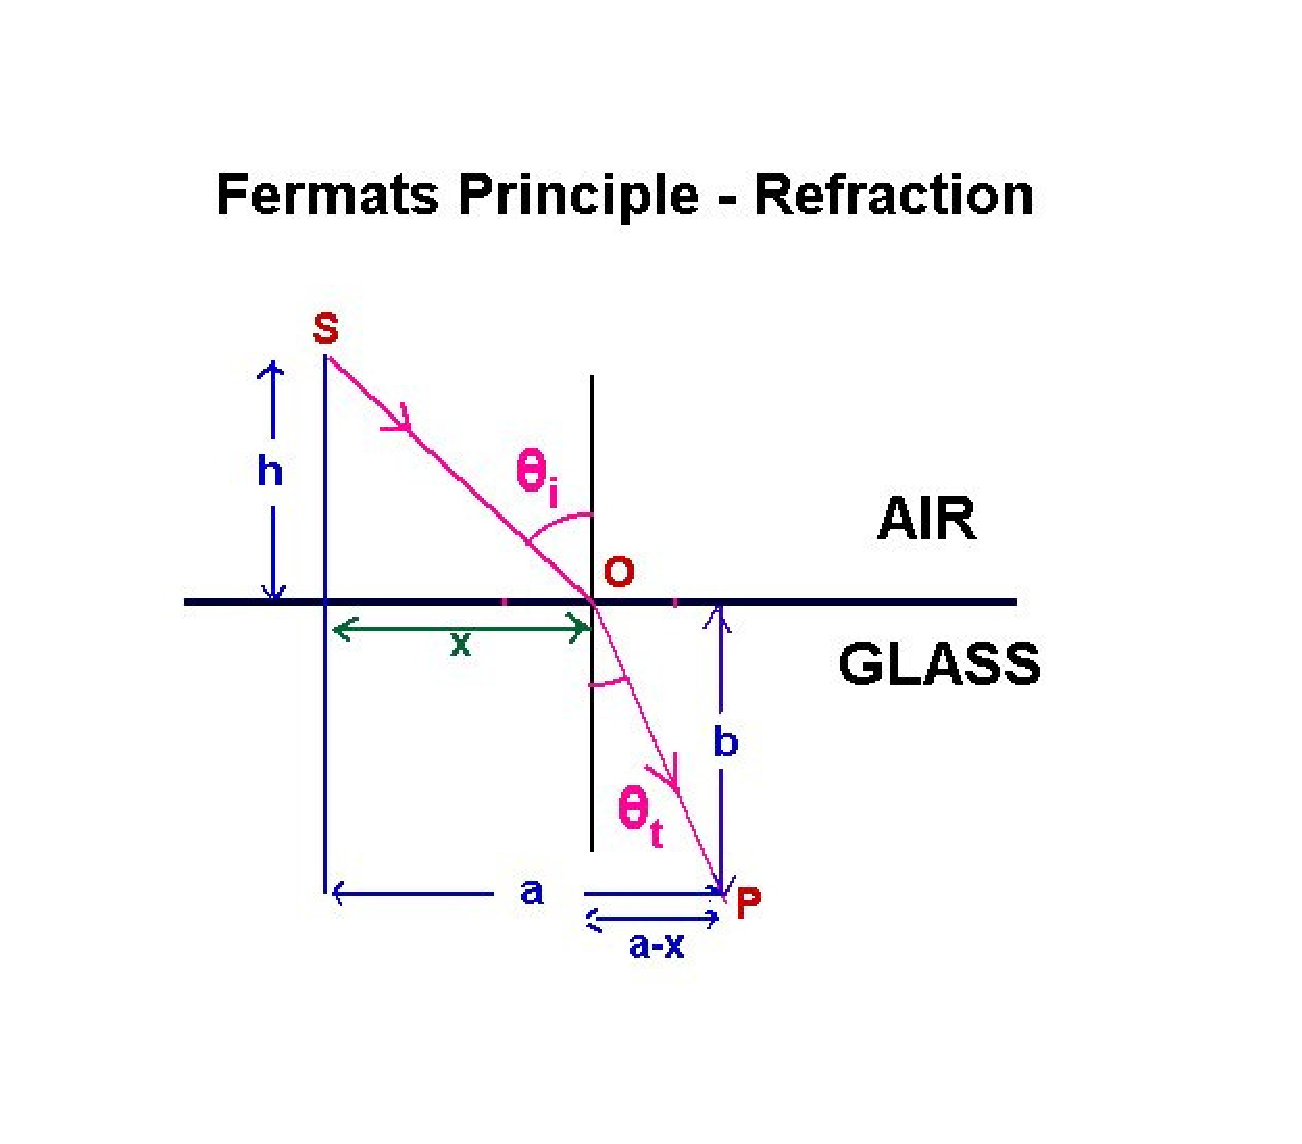
\includegraphics[scale=0.5]{image-1.eps}
\end{figure}

Optical path from $S$ to $P$:

\begin{equation*}
L=n_a\sqrt{x^2+h^2}+n_g\sqrt{(a-x)^2+b^2}
\end{equation*}
\begin{equation*}
\frac{dL}{dx}=0
\end{equation*}
\begin{equation*}
\frac{dL}{dx} = \frac{n_ax}{\sqrt{x^2+h^2}} + \frac{n_g(x-a)}{\sqrt{(a-x)^2+b^2}} = 0
\end{equation*}
\begin{equation*}
\frac{n_ax}{\sqrt{x^2+h^2}} = \frac{n_g(x-a)}{\sqrt{(a-x)^2+b^2}}
\end{equation*}
\begin{equation}\boxed{
n_a\sin{\theta_i} = n_g\sin{\theta_t}
}\end{equation}
which is Snell's law.

\subsection{Lenses}
Lenses are devices which modify the curvature of a wavefront.
\begin{figure}[h!]
\centering
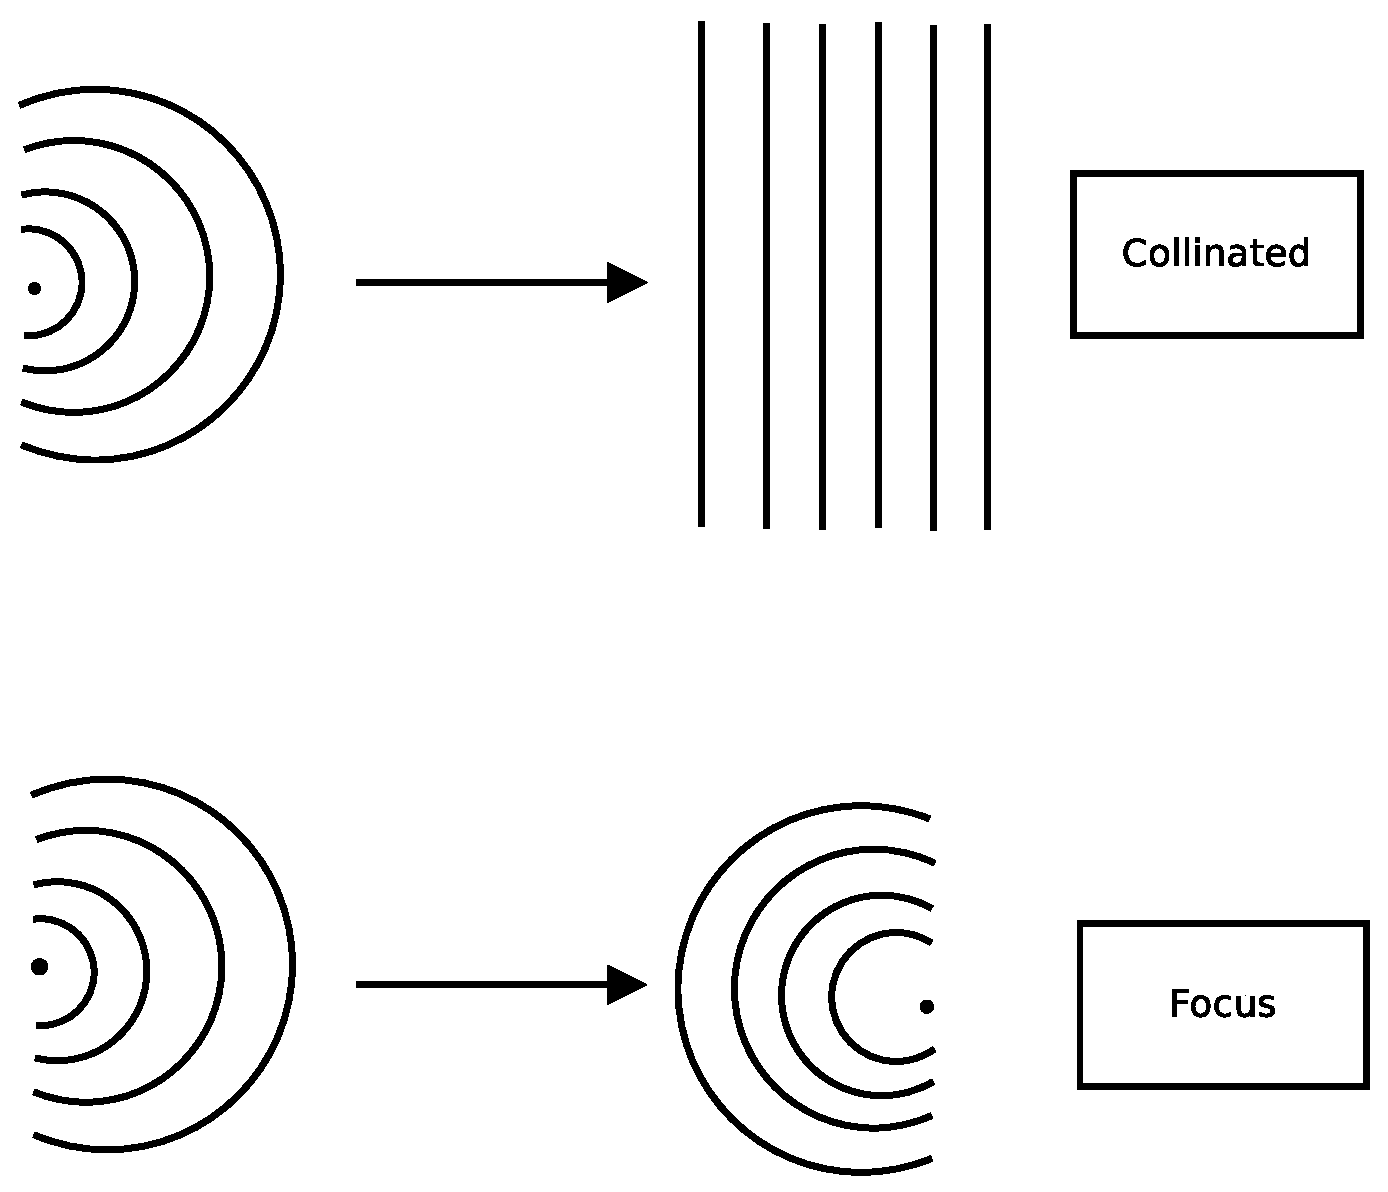
\includegraphics[scale=0.3]{Rays3.eps}
\end{figure}

\subsubsection{Refraction at a spherical surface}
\begin{figure}[h!]
\centering
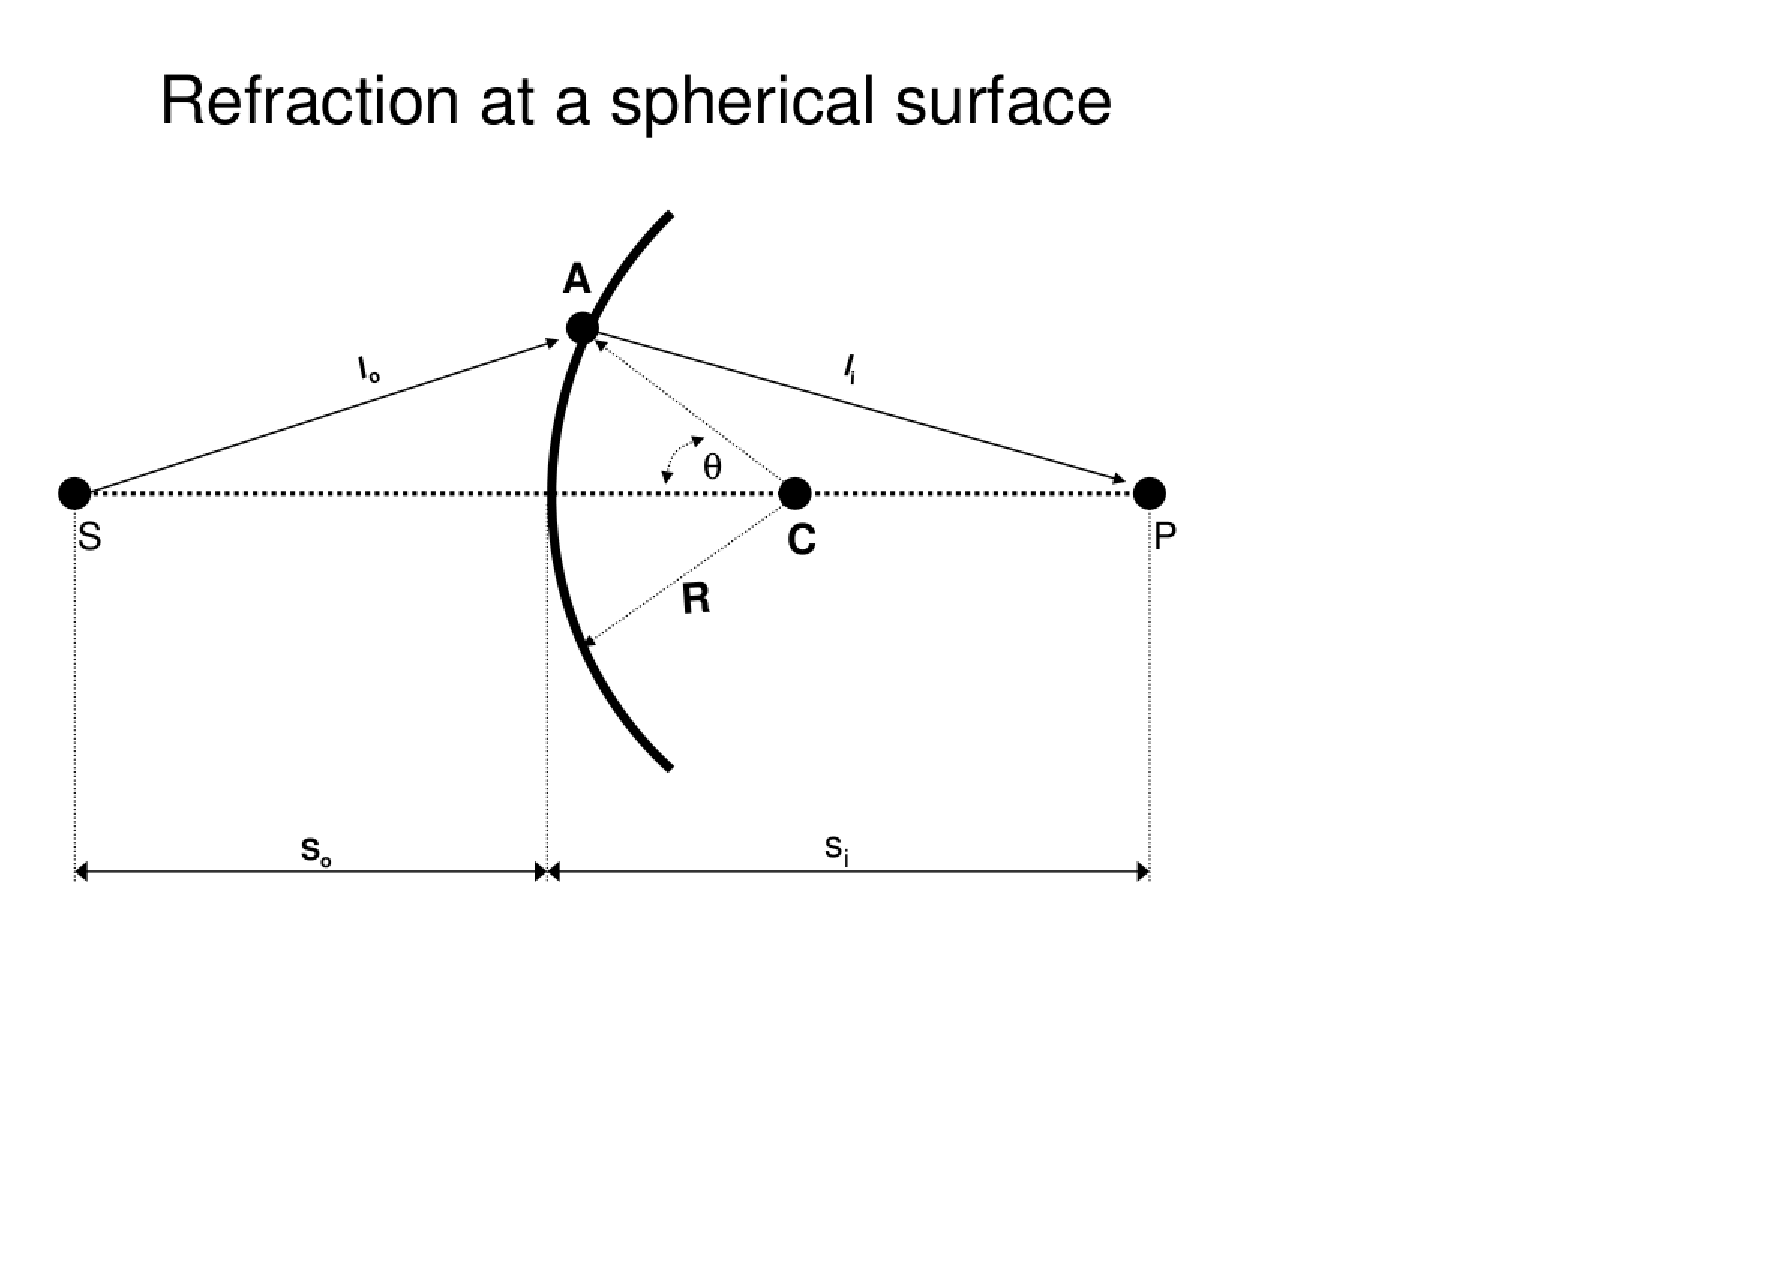
\includegraphics[scale=0.5]{image-2.eps}
\end{figure}
The optical path length from $S$ to $P$ via $A$:
\begin{equation*}
L=n_ol_o+n_il_i
\end{equation*}
\begin{equation*}
l_o ^2 = (s_o + R)^2 + R^2 - 2R(s_o +R)\cos{\theta}
\end{equation*}
\begin{equation*}
l_i ^2 = (s_i - R)^2 + R^2 - 2R(s_i -R)\cos{180 - \theta}
\end{equation*}
\begin{equation*}
l_i ^2 = (s_i - R)^2 + R^2 + 2R(s_i -R)\cos{\theta}
\end{equation*}
By Fermat Principle:
\begin{equation*}
\frac{dL}{d\theta} = 0
\end{equation*}
\begin{equation*}
\frac{dL}{d\theta} = \frac{n_o R(s_o + R)\sin{\theta}}{l_o} - \frac{n_i R(s_i - R)\sin{\theta}}{l_i}
\end{equation*}
\begin{equation*}
n_o\frac{s_o + R}{l_o} = n_i\frac{s_i - R}{l_i}
\end{equation*}

For small $\theta$, $l_o \approx s_o$ and $l_i \approx s_i$ -- the \textit{paraxial approximation}, also known as first order approximation and Gaussian Optics.
\begin{equation*}
n_o(1 + \frac{R}{s_o}) - n_i(1 - \frac{R}{s_i})
\end{equation*}
\begin{equation}\boxed{
\frac{n_o}{s_o} + \frac{n_i}{s_i} = \frac{n_i - n_o}{R}
}\end{equation}
\textbf{Note:} There is no $\theta$ dependence: all rays from $S$ converge at $P$.

In general, because of the spherical symmetry, \underline{all} rays from any object will converge on a converge on a corresponding image point $P$.
\begin{itemize}
\item There is a unique mapping from object to image.
\item The optical field in the object is reproduced in the image plane.
\end{itemize}

\subsubsection{Reflection by a lens}
\begin{figure}
\centering
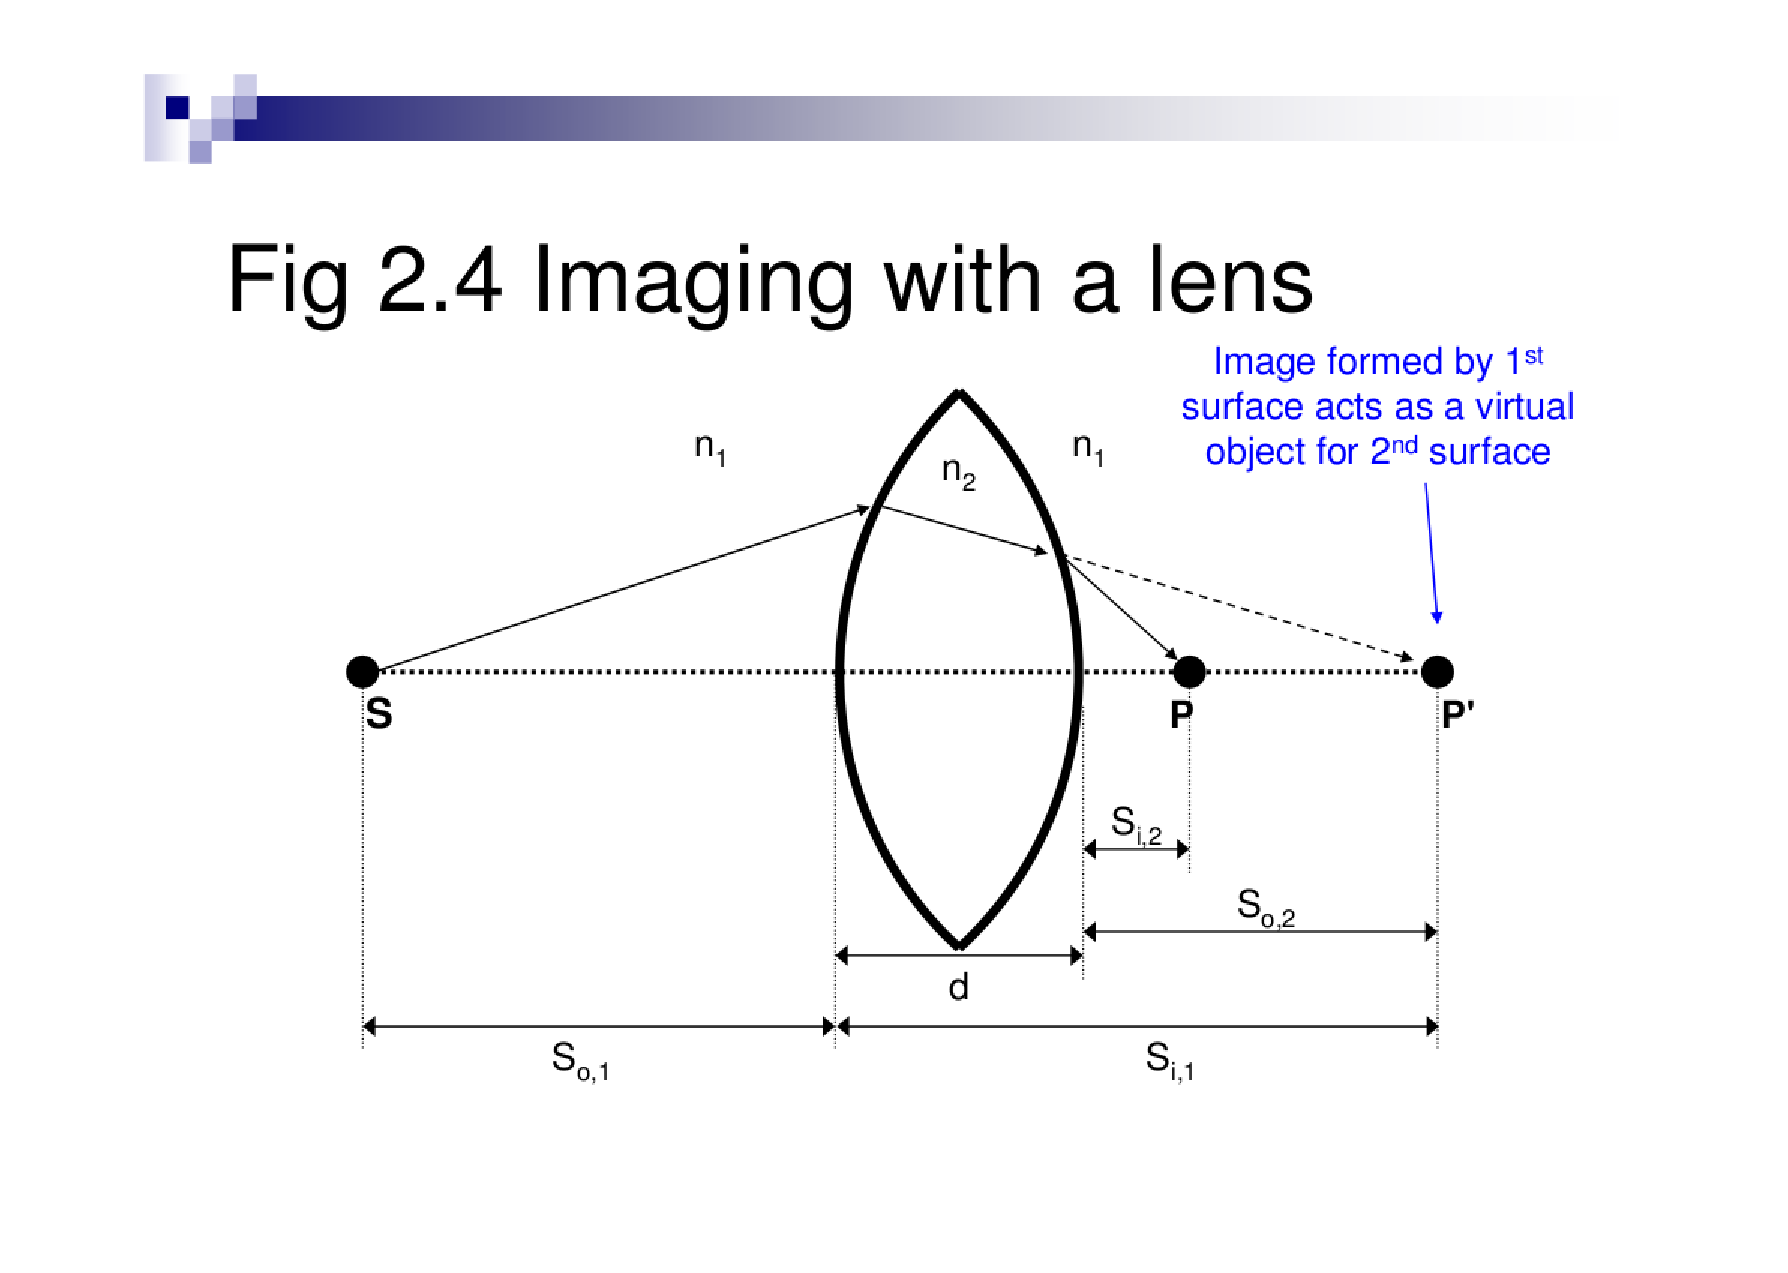
\includegraphics[scale=0.5]{Geo.eps}
\end{figure}
Image from the first surface acts as an object for the second surface.

For the first surface:
\begin{equation*}
\frac{n_1}{s_{o_1}} + \frac{n_2}{s_{i_1}} = \frac{n_2 - n_1}{R_1}
\end{equation*}
For the second surface:
\begin{equation*}
\frac{n_2}{s_{o_2}} + \frac{n_1}{s_{i_2}} = \frac{n_1 - n_2}{R_2}
\end{equation*}
\begin{equation*}
|s_{o_2}| = s_{i_1} - d
\end{equation*}
but $P'$ is to the right of the lens (virtual object):
\begin{equation*}
s_{o_2} \leq 0
\end{equation*}
\begin{equation*}
s_{o_2} = d - s_{i_1}
\end{equation*}
Using above expressions, get
\begin{equation*}
\frac{1}{s_{o_1}} + \frac{1}{s_{i_1}} = \frac{n_2 - n_1}{n_1}(\frac{1}{R_1} - \frac{1}{R_2}) + \frac{n_2}{n_1}\frac{d}{s_{i_1}(s_{i_1} - d)}
\end{equation*}
For a thin lens $d \longrightarrow 0$:
\begin{equation*}
s_{o_1} = u
\end{equation*}
\begin{equation*}
s_{i_1} = v
\end{equation*}
\begin{equation}\boxed{
\frac{1}{u} + \frac{1}{v} = \frac{n_2 - n_1}{n_1}\left(\frac{1}{R_1} - \frac{1}{R_2}\right)
}\end{equation}
That's the lensmaker's formula.

Rewrite as
\begin{equation}\boxed{
\frac{1}{u} + \frac{1}{v} = \frac{1}{f}
}\end{equation}
$f$ -- focal length.

For a convex lens: $f > 0$.

For a concave lens: $f < 0$.

\begin{figure}
\centering
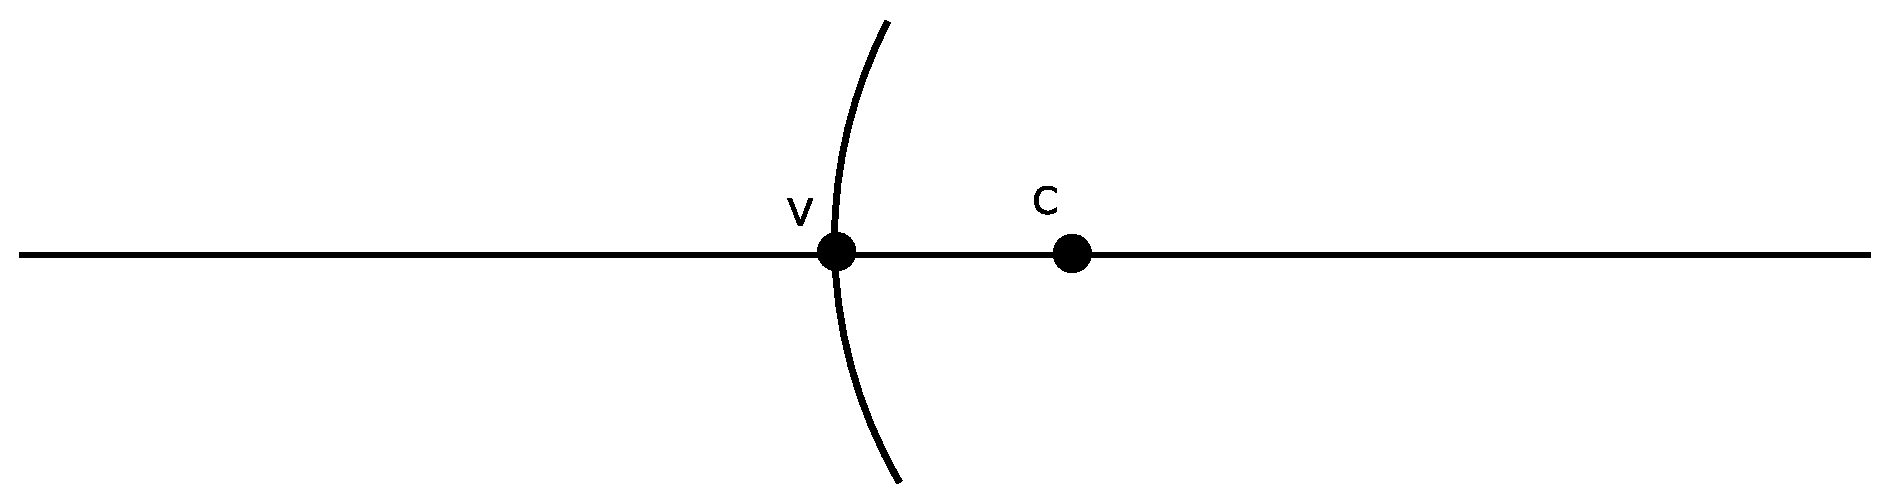
\includegraphics[scale=0.35]{Diagram1.eps}
\end{figure}
$V$ -- vertex.

$C$ -- centre of curvature.

Sign convention:
\begin{itemize}
\item $u$ is positive, if it is on the \textit{left} of $V$ (real object);
\item $u$ is negative, if it is on the \textit{right} of $V$ (virtual object);
\item $v$ is positive, if it is on the \textit{right} of $V$ (real image);
\item $v$ is negative, if it is on the \textit{left} of $V$ (virtual image);
\end{itemize}
\begin{tabular}{c l l}
$R$ & if $C$ is on the right & if $C$ is on the left\\
$f$ & positive & negative\\
 & converging & diverging\\
\end{tabular}

\subsection{Spherical mirrors}
\begin{equation}\boxed{
\frac{1}{s_o} + \frac{1}{s_i} = \frac{2}{R} = \frac{1}{f}
}\end{equation}

Sign convention for mirrors is same as for a lens, except that concave mirror is converging light ($f > 0$) and convex mirror causes light to diverge ($f < 0$).

\subsection{Ray Diagrams}
To construct a ray diagram, draw two out of three rays:
\begin{enumerate}
\item Straight through the centre;
\item Initially parallel to axis, then to focus;
\item Through the focus, then parallel to the axis.
\end{enumerate}

Magnification.

Magnification $M$ is equal to
\begin{equation}\boxed{
M = -\frac{y_i}{y_o}
}\end{equation}
negative because inverted.
\begin{figure}[h!]
\centering
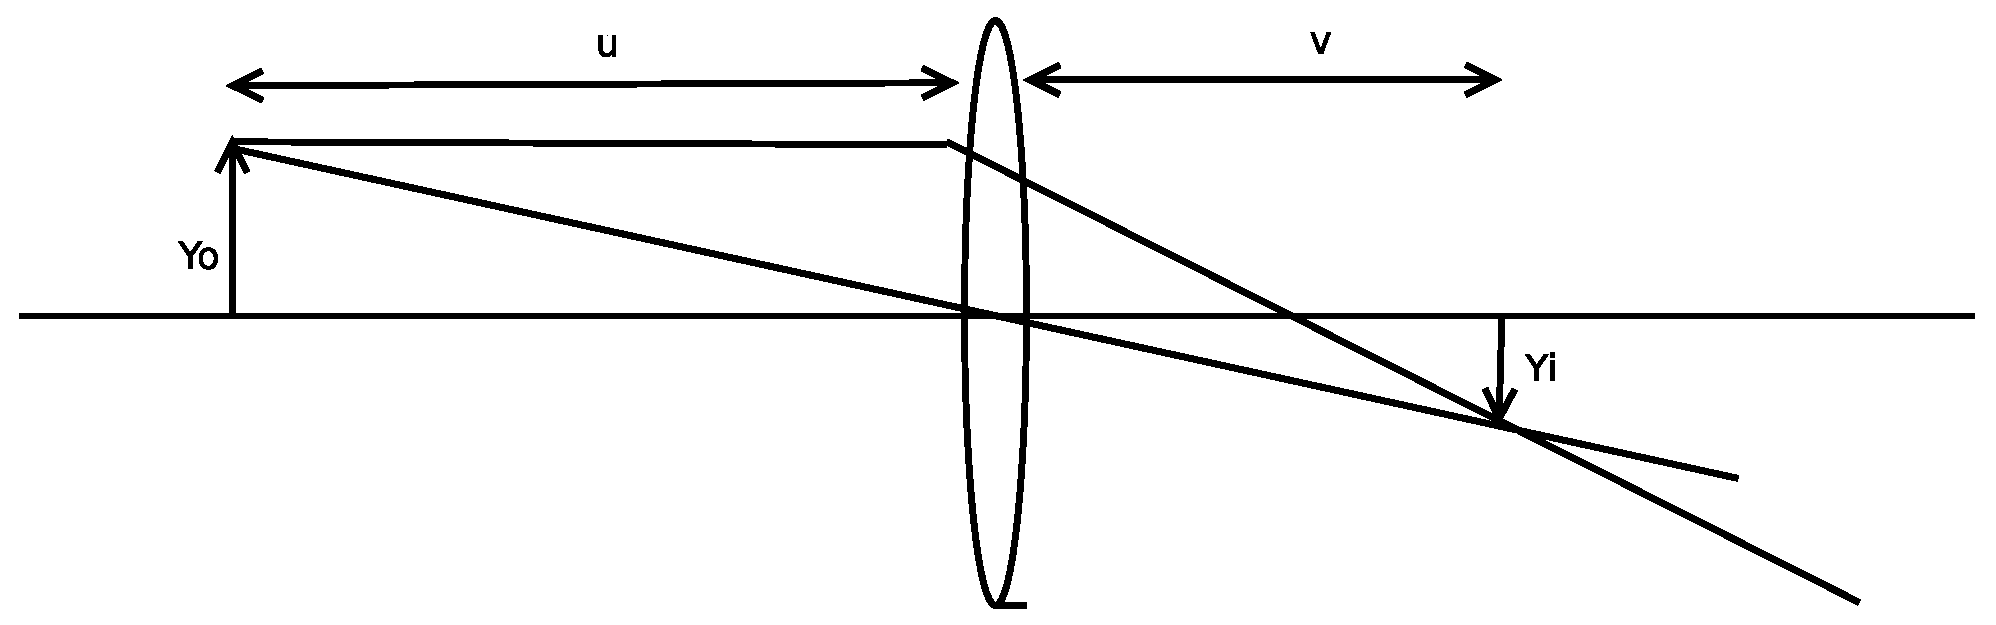
\includegraphics[scale=0.35]{m.eps}
\end{figure}

Because of the similarity of triangles:
\begin{equation}\boxed{
M = -\frac{v}{u}
}\end{equation}

If $M < 0$, then the image is inverted, if $M > 0$, then the image is upverted.

$|M|>1$ -- magnified.

$|M|<1$ -- minified.

\subsection{Optical Instruments}
\subsubsection{The eye}
When eye is relaxed, its lens focuses light from $\infty$ onto retina.

More compatible to view images when eye is relaxed, therefore optical instruments are designed to produce $v = \infty$ but 
\begin{equation*}
M = -\frac{v}{u}
\end{equation*}
therefore
\begin{equation*}
M = \infty
\end{equation*}
$\Rightarrow$ need alternate definition.

\subsubsection{Magnifying power. Angular magnification}
\begin{equation*}
MP = \frac{\mbox{size of retined image thro instrument}}{\mbox{size of natural image with naked eye at natural viewing distance}}
\end{equation*}
Size of retined image $\alpha$ angle undeflected ray makes with central axis.
\begin{figure}[h!]
\centering
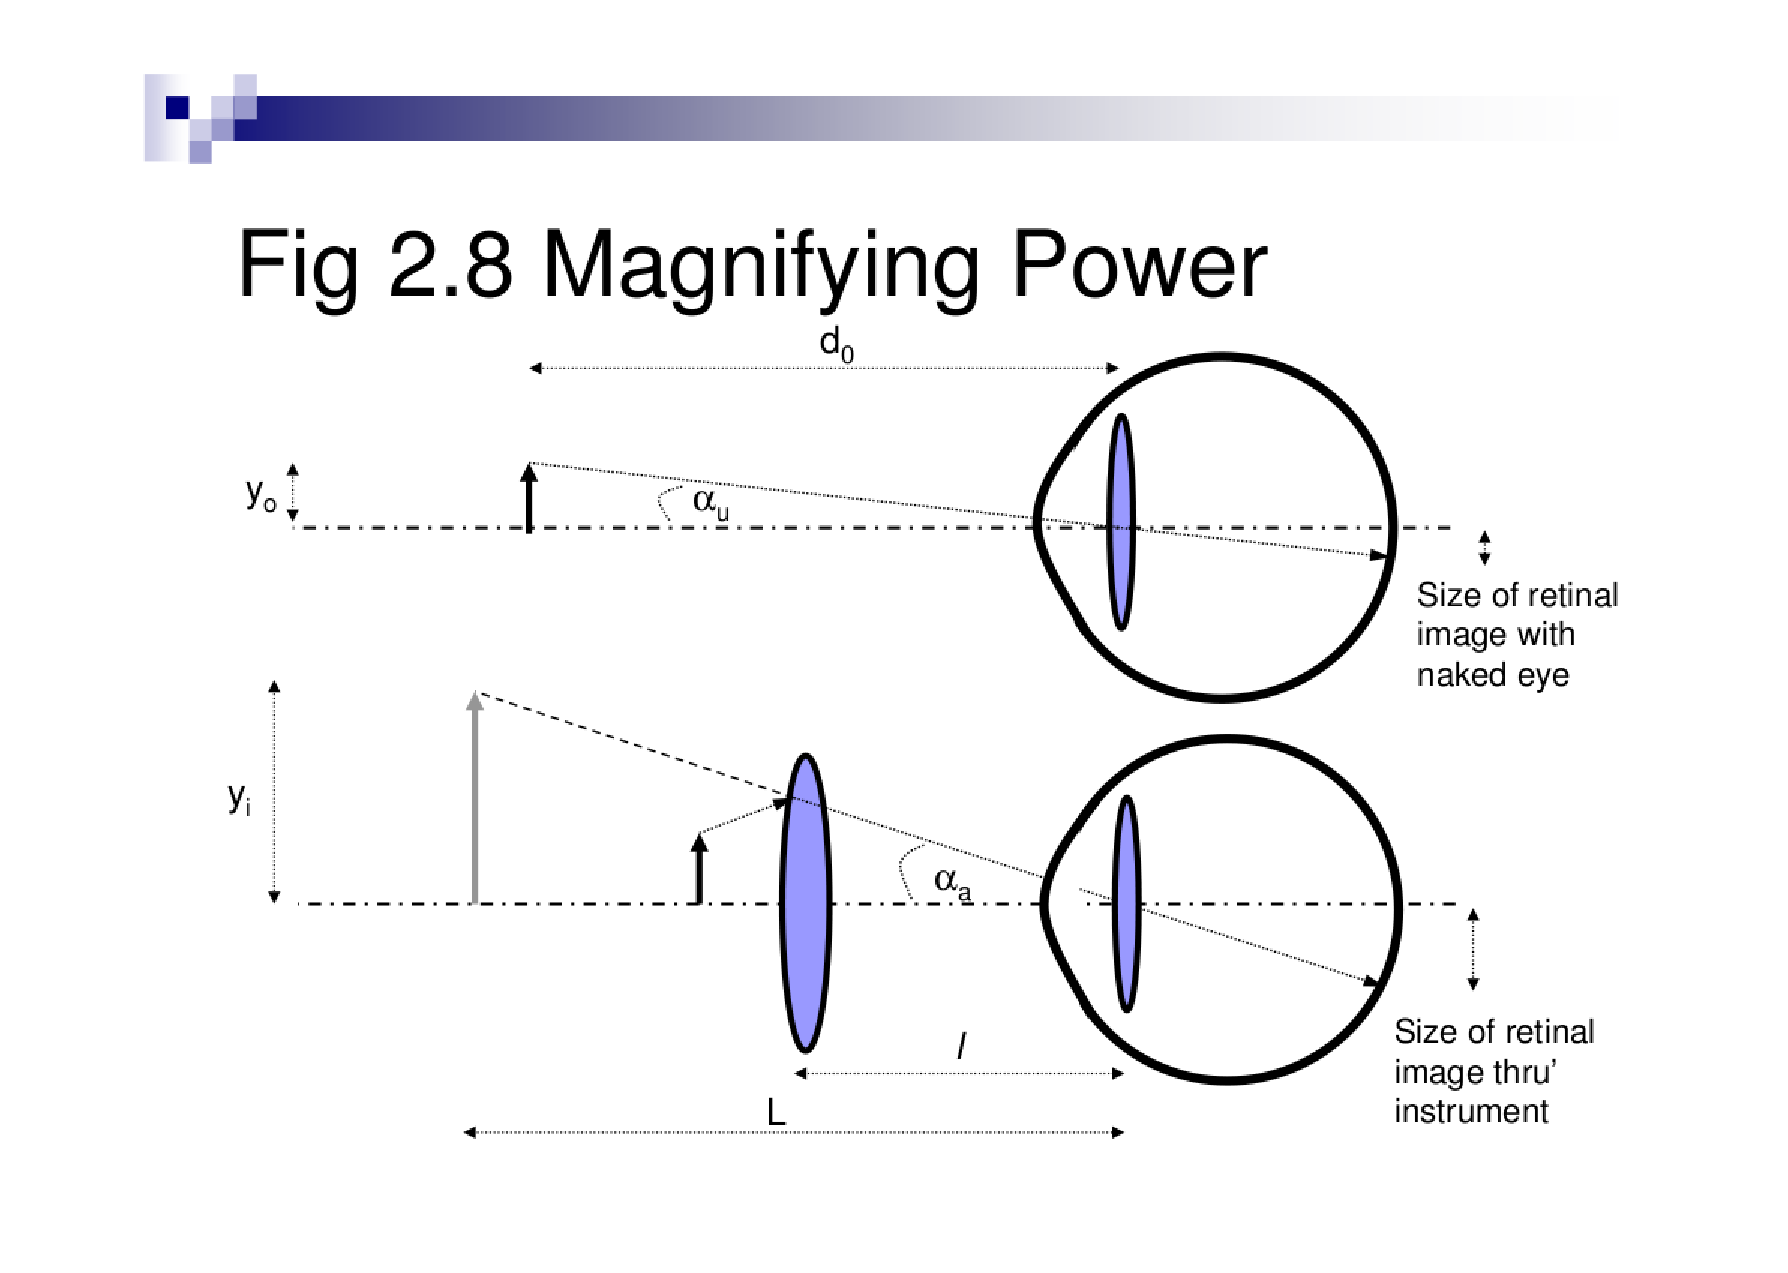
\includegraphics[scale=0.5]{MP.eps}
\end{figure}
\begin{equation*}
MP = \frac{\alpha_a}{\alpha_u}
\end{equation*}
\begin{equation*}
\tan{\alpha_a} = \frac{y_o}{L} \approx \alpha_a
\end{equation*}
\begin{equation*}
\tan{\alpha_u} = \frac{y_i}{d_0} \approx \alpha_u
\end{equation*}
\begin{equation*}
MP = \frac{y_i}{y_o} \frac{d_0}{L}
\end{equation*}
\begin{equation*}
MP = \frac{d_0}{L} (1 - \frac{v}{f})
\end{equation*}
but
\begin{equation*}
v = - (L - L) = l - L
\end{equation*}
$v < 0$ since it's left of lens.
\begin{equation}\boxed{
MP = \frac{d_0}{L} (1 + \frac{L-l}{f})
}\end{equation}
For an image at $\infty$
\begin{equation*}
u=f
\end{equation*}
\begin{equation*}
L=\infty
\end{equation*}
formulae reduces:
\begin{equation*}
[MP]_\infty = \frac{d_0}{f}
\end{equation*}

\subsubsection{The microscope}
\begin{figure}[h!]
\centering
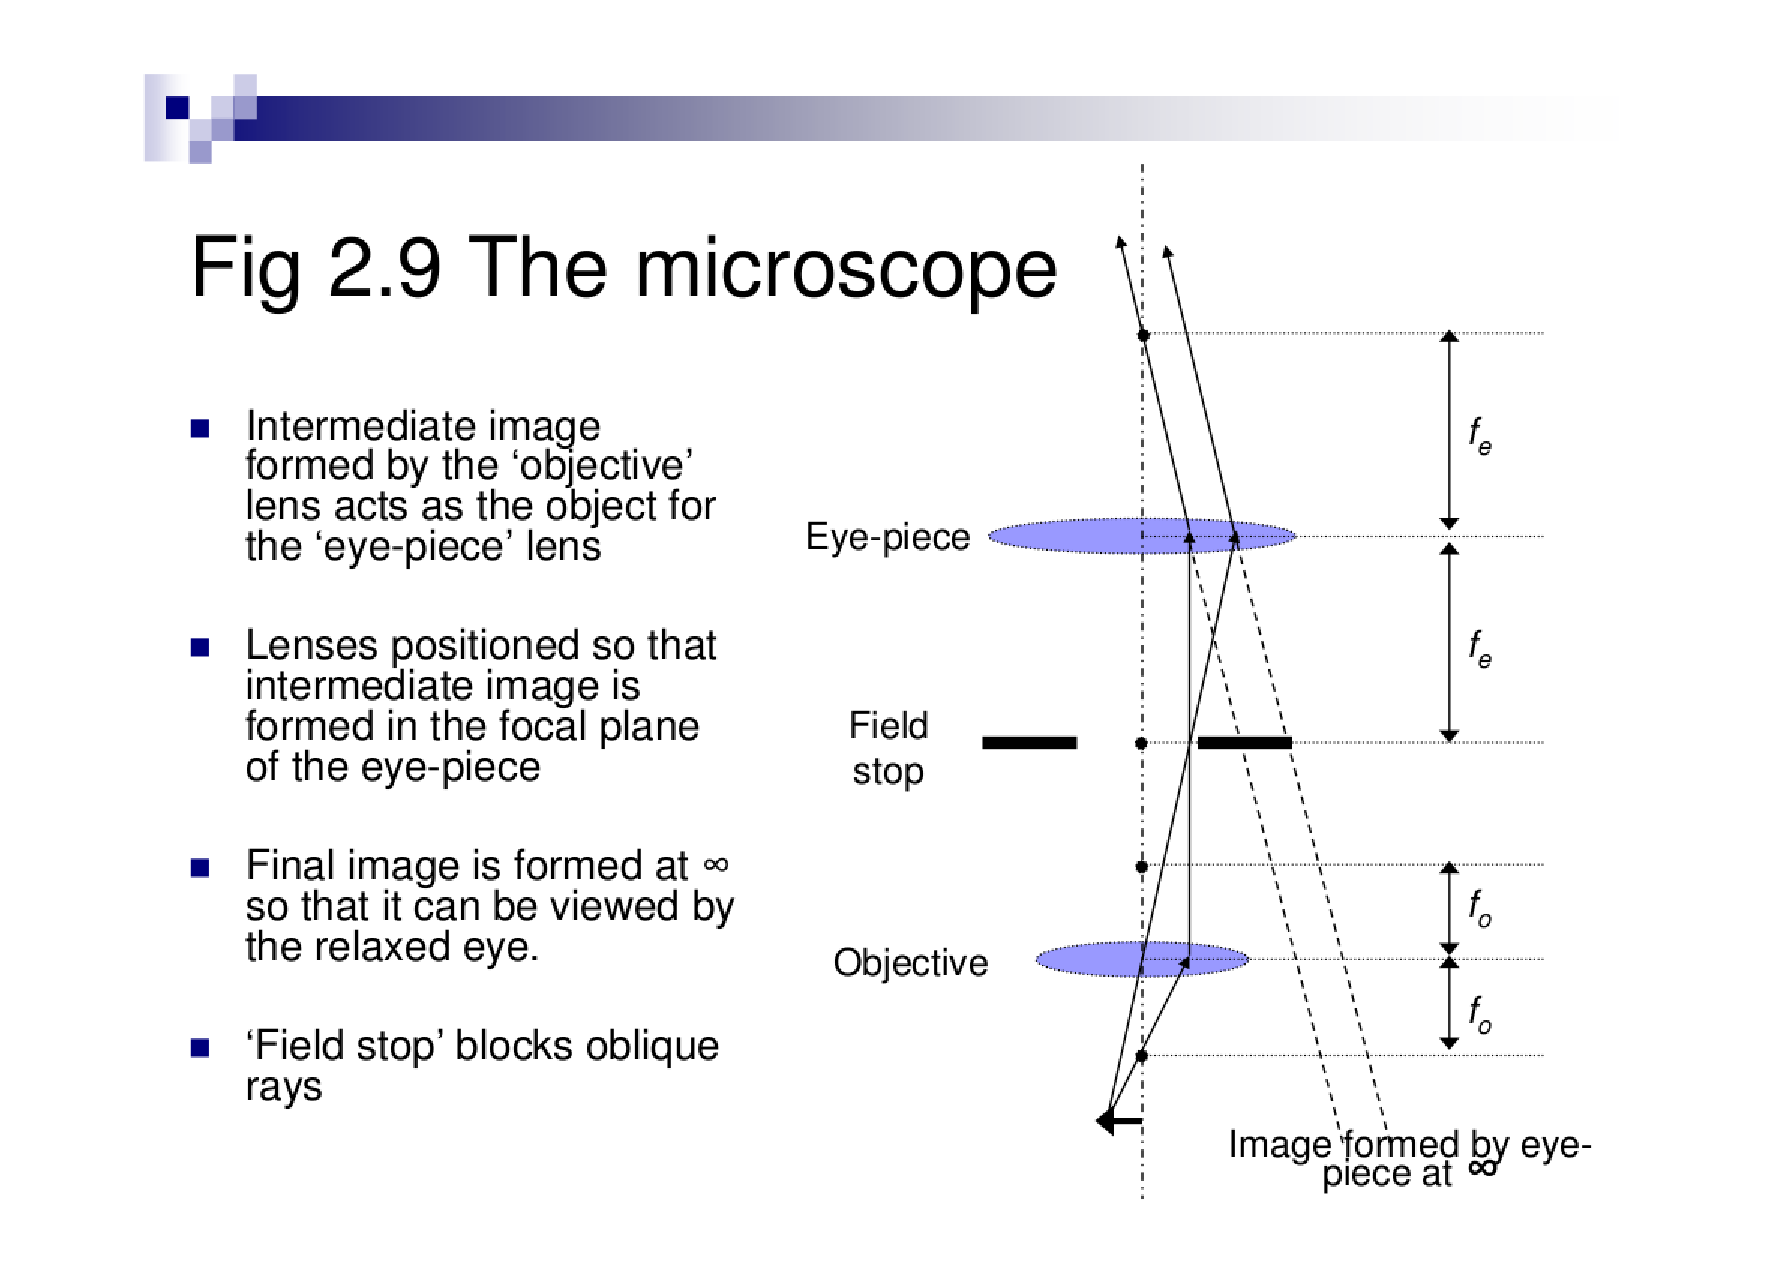
\includegraphics[scale=0.5]{m2.eps}
\end{figure}
\begin{itemize}
\item Objective forms a real image of the object
\begin{equation}\boxed{
M_o = - \frac{v}{u} \approx -5
}\end{equation}
this image acts as the object for the eyepiece (ocular).
\item Lenses are arranged so that the image forms in the focal plane of eyepiece $\Rightarrow$ fixed image at $\infty$.
\begin{equation*}
[MP]_e = \frac{d_0}{f} \sim \times 10
\end{equation*}
\begin{equation*}
[MP]_T = [MP]_e M_o \sim -50
\end{equation*}
\end{itemize}

Field stops block oblique rays that distorted or blur image.

\textbf{Note:} Paraxial approximation is \underline{no} longer valid: lens eqs are \underline{not} valid.

\subsubsection{The telescope}
\begin{figure}[h!]
\centering
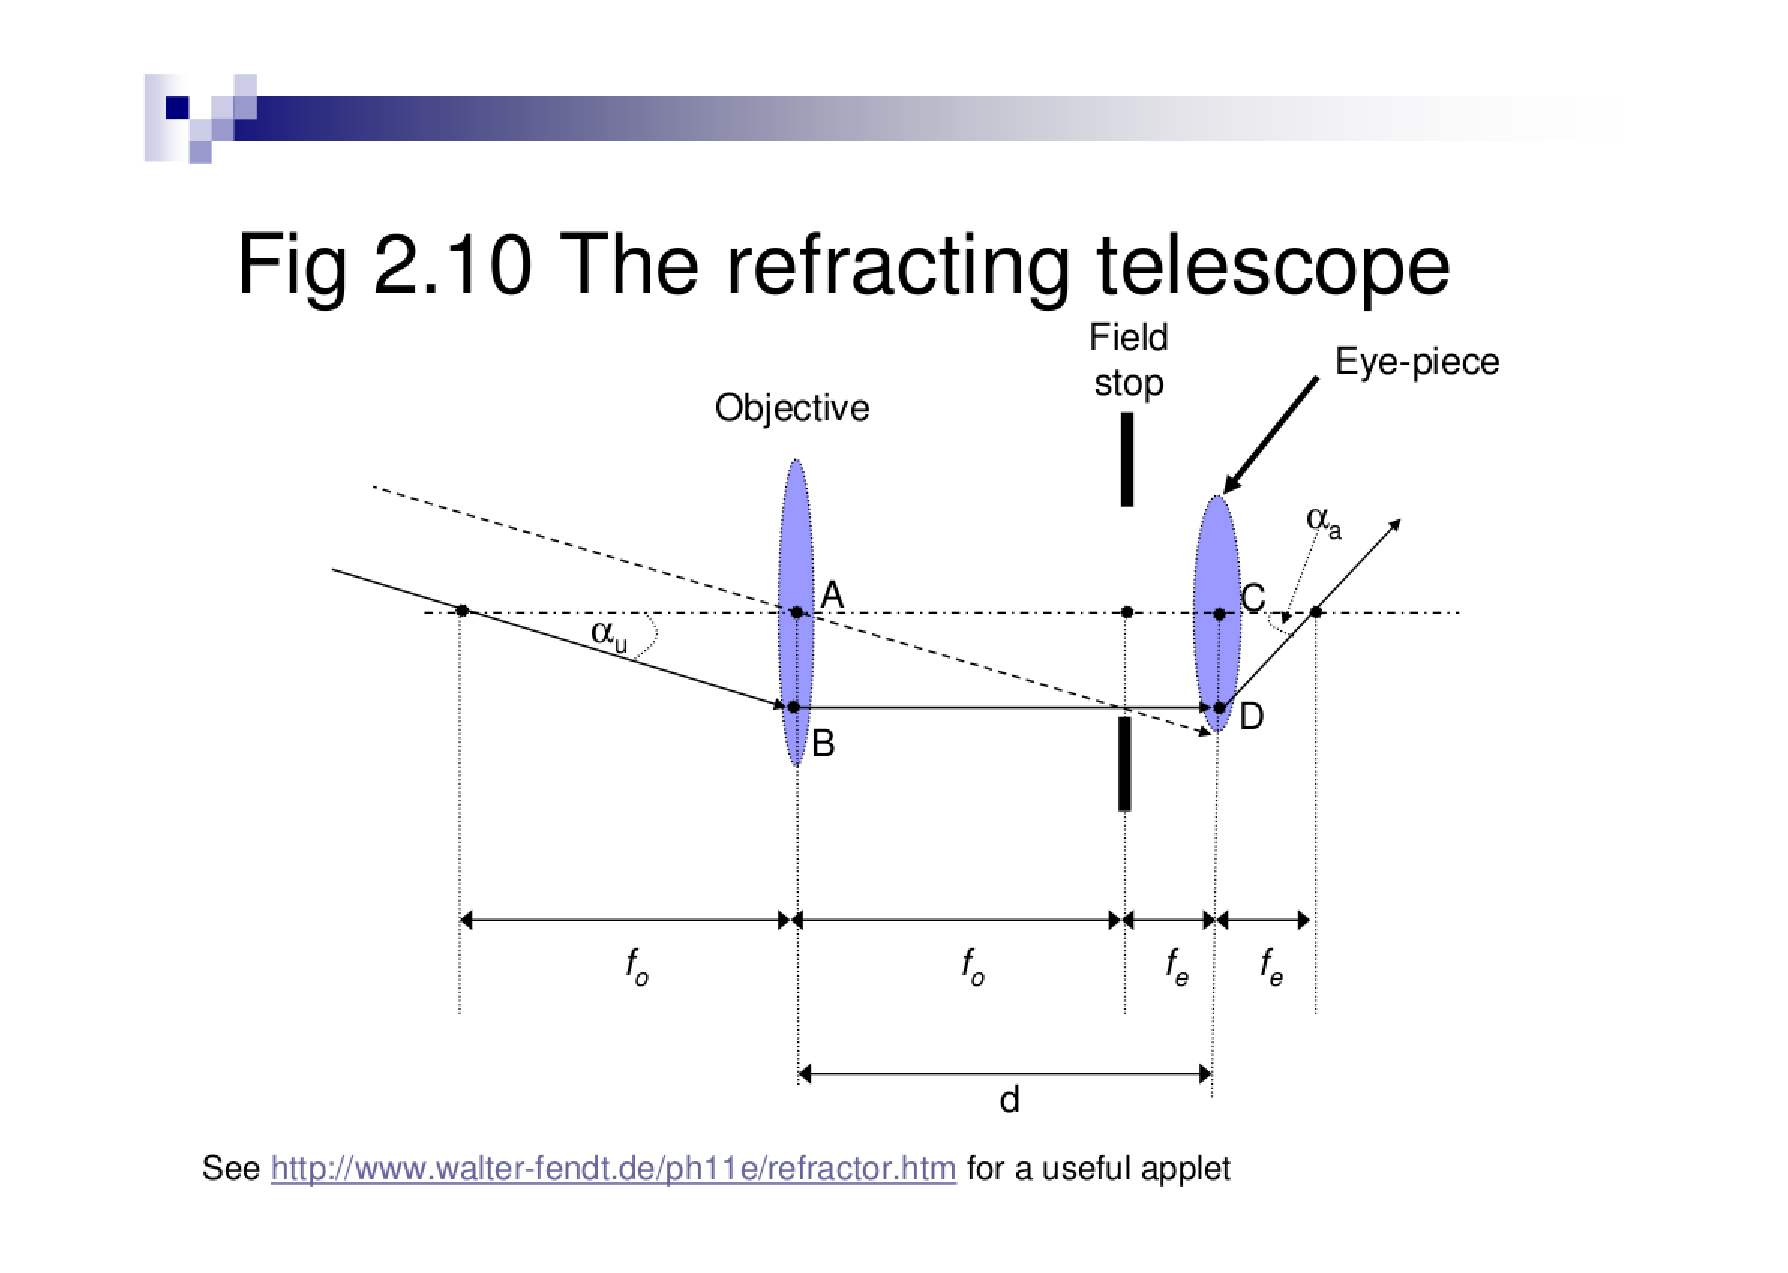
\includegraphics[scale=0.5]{m3.eps}
\end{figure}
\begin{itemize}
\item Similar principle to microscope.
\item Objective forms an image which acts object for the eyepiece.
\item Final image is formed at infinity, so it can be viewed by relaxed eye.
\item But now object is at $\infty$, so interpretate image formed at $f_0$.
\item Lens superposition: $d = f_o + f_e$.
\end{itemize}

$MP$ of a telescope.

Consider a ray through the first focus of objective.
\begin{equation*}
MP = -\frac{\alpha_a}{\alpha_u}
\end{equation*}
it is $<0$, because image is inverted.
\begin{equation*}
\tan{\alpha_a} = \frac{CD}{f_e} \approx \alpha_a
\end{equation*}
\begin{equation*}
\tan{\alpha_u} = \frac{AB}{f_o} \approx \alpha_u
\end{equation*}
but
\begin{equation*}
AB=CD
\end{equation*}
\begin{equation}\boxed{
MP = -\frac{f_o}{f_e}
}\end{equation}

Why are reflectors better than reflectors?

The whole lens has to be deflect-free whereas only front surface of a mirror need to be perfect.

In a lens
\begin{equation*}
n = f(\lambda)
\end{equation*}
therefore focal length
\begin{equation*}
f = f(\lambda)
\end{equation*}
$\Rightarrow$ chromatic abberation.

A large lens must be supported at edges. A mirror can be supported underneeth.

\subsubsection{Gravitational lensing}
General relativity $\Rightarrow$ mass curves space-time. In a curved space-time, shortest path is no longer a straight line, therefore light follows a curve. $\Rightarrow$ passing through lens.
\begin{figure}[h!]
\centering
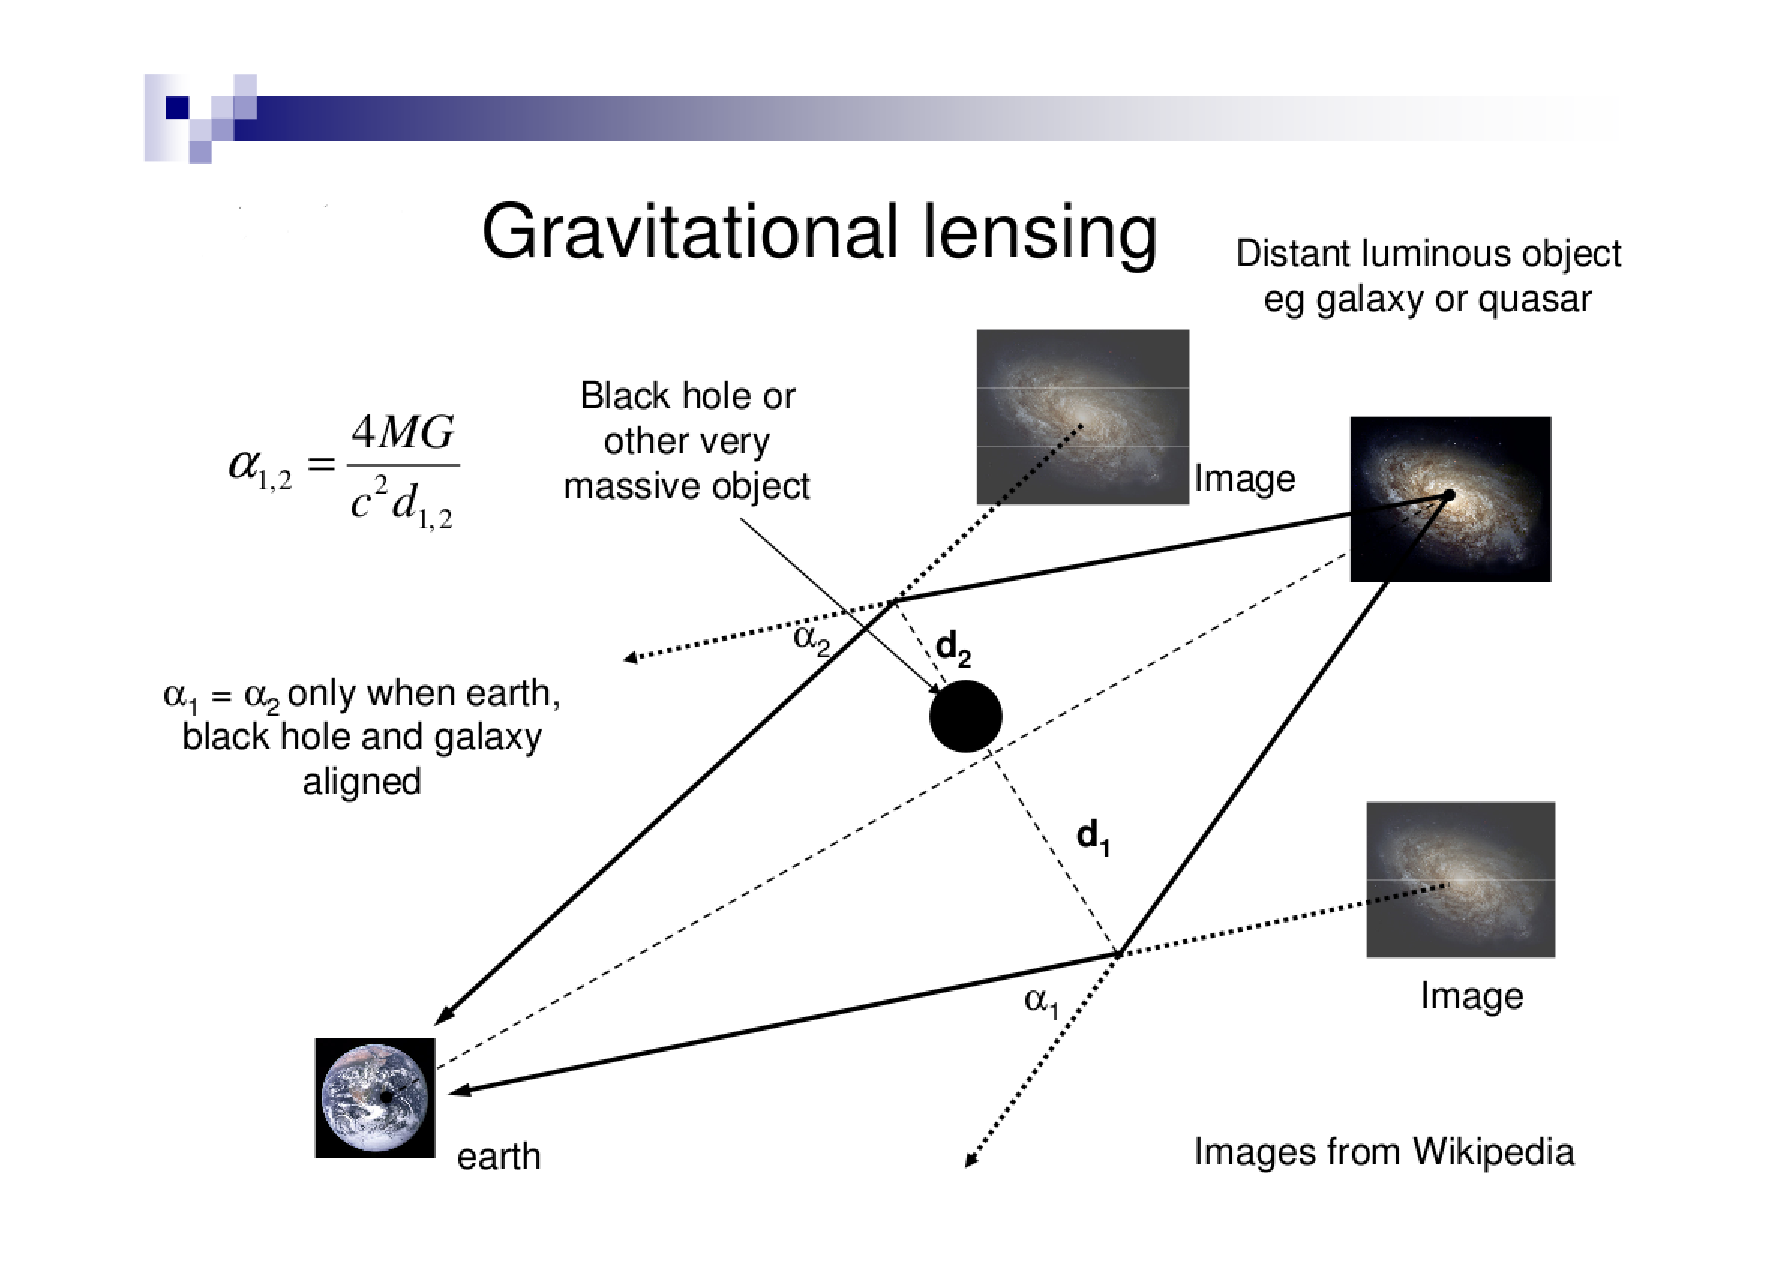
\includegraphics[scale=0.5]{m4.eps}
\end{figure}

\section{Polarisation}
\subsection{Polarisation states}
For a wave propagating in $z-$direction:
\begin{equation*}
\vec{E_x} = \hat{x}E_x e^{{i(kz- \omega t)}}
\end{equation*}
\begin{equation*}
\vec{E_y} = \hat{y}E_y e^{i(kz- \omega t + \phi)}
\end{equation*}

\begin{itemize}
\item[(i)] \textit{Linear polarisation.} $\vec{E_x}$ and $\vec{E_y}$ components are either in phase or in anti-phase ($\phi = 0$ or $\phi = \pi$)
\item[(ii)] \textit{Circular polarisation.} $\vec{E_x}=\vec{E_y}$ and they are out of phase by $\pm \frac{\pi}{2}$.

$\phi=\frac{\pi}{2}$ -- Left circular polarisation

$\phi=-\frac{\pi}{2}$ -- Right circular polarisation

\textbf{N.B.:} For an observer looking towards source, $\vec{E}$ rotates clockwise for RH.
\item[(iii)] \textit{Elliptical polarisation.} $\vec{E_x} \neq \vec{E_y}$, $\phi$ is arbitary.
\item[(iv)] \textit{Unpolarised light.} Unsynchronised emission from atoms/molecules in natural situations. It still has instant polarisation changes randomly and too rapidly to measure $\Rightarrow$ polarisation “smears" out.
\item[(v)] \textit{Partial polarisation.}
\begin{itemize}
\item[-] intermediate between pol. and unpol.;
\item[-] polarisation changes rapidly, but tends to a particular direction.
\end{itemize}
\end{itemize}

\subsection{Polarisation by reflection and scattering}
Both are a consequence of anisotropic emission of dipoles and in particular nothing is emmited parallel to original $\vec{E}$.

\subsubsection{Polarisation by reflection.}
Reflectivity is polarisation dependent, so
\begin{equation*}
\frac{E_p}{E_s} \vert_i \neq \frac{E_p}{E_s} \vert_r
\end{equation*}
There are two cases:
\begin{itemize}
\item[$\bullet$] $\vec{E}$ is perpendicular to the plane of incidence; s-polarised; emission is always $max$ in direction of $\vec{E_z}$
\item[$\bullet$] $\vec{E}$ is parallel to the plane of incidence; p-polarised; emission aplitude varies with the direction of $\vec{E_z}$
\end{itemize}

\subsubsection{Brewster angle}
At certain angle, axis of induced dipole (perpendicular to transmitted ray) will be such that nothing is reflected.
\begin{figure}[h!]
\centering
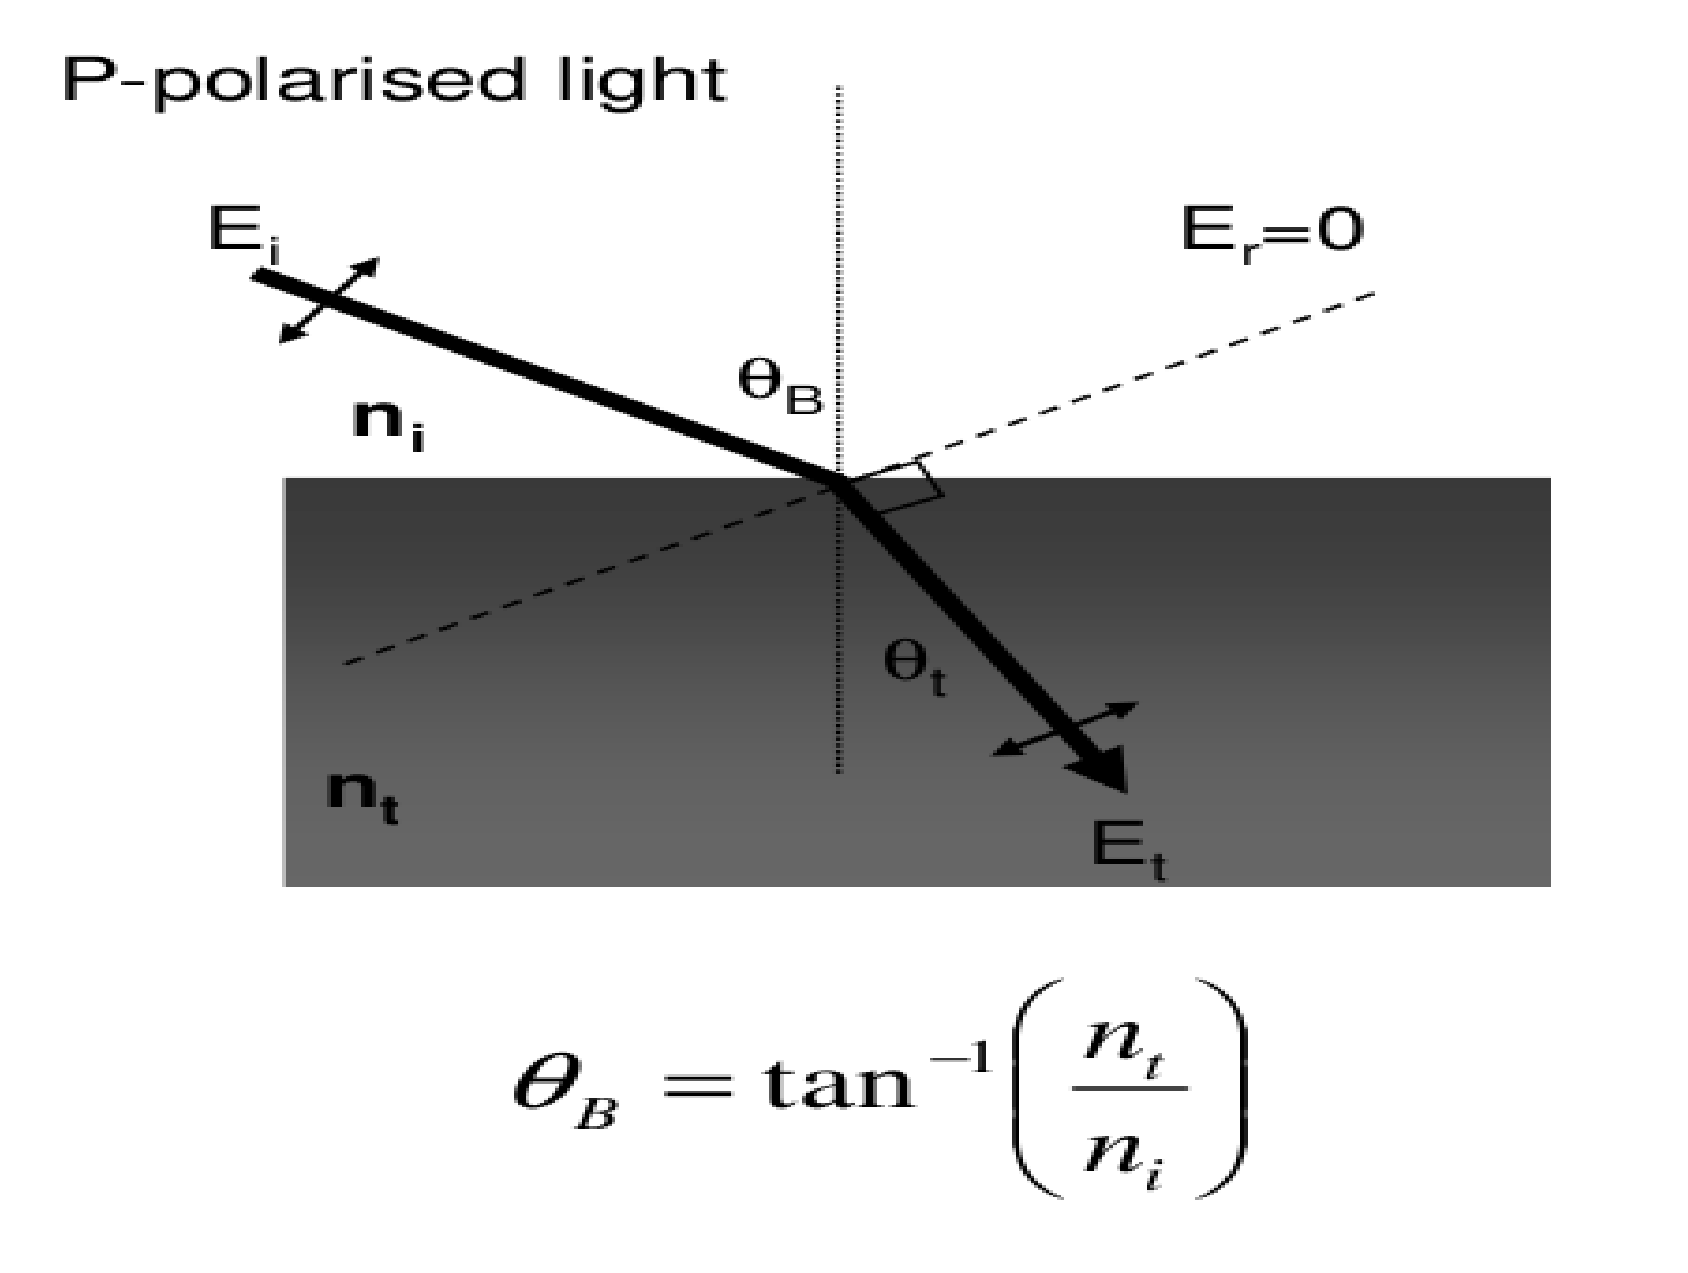
\includegraphics[scale=0.25]{tew.eps}
\end{figure}

Zero amplitude:
\begin{equation*}
\theta_i + \theta_r = \frac{\pi}{2}
\end{equation*}
this incidence angle is called either polarisation angle or Brewster's angle.
\begin{equation*}
\theta_B + \theta_r = \frac{\pi}{2}
\end{equation*}

Snell's law:
\begin{equation*}
n_i \sin{\theta_B} = n_r \sin{\theta_r}
\end{equation*}
\begin{equation*}
n_i \sin{\theta_B} = n_r \sin{\frac{\pi}{2} - \theta_B}
\end{equation*}
\begin{equation*}
n_i \sin{\theta_B} = n_r \cos{\theta_B}
\end{equation*}
\begin{equation*}
\frac{n_r}{n_i} = \tan{\theta_B}
\end{equation*}
\begin{equation}\boxed{
\theta_B = \tan^{-1}{\frac{n_r}{n_i}}
}\end{equation}

\subsubsection{Polarisation by scattering}
\begin{itemize}
\item[$\bullet$] Optical electric field induces dipole in atom/molecule.
\item[$\bullet$] For polarised light, polarisation is maintained but amplitude of scattered light changes with direction.
\item[$\bullet$] For unpolarised light, polarisation state changes with direction.
\end{itemize}

\subsection{Dichroism}
Some materials selectively absorb one polarisation direction, e.g. polaroid sheet consist of aligned, long thin molecules. So $E_{\parallel}$ to long axis does not work is moving charge up and down molecule and is absorbed. $E_{\perp}$ to long axis does little work and is not absorbed. Transmitted field component is $E \cos{\theta}$. Transmitted intensity:
\begin{equation}\boxed{
I(\theta) = I_0 \cos^2{\theta}
}\end{equation}
That's called Malus' Law.

\subsection{Optical Anisotropy}
\subsubsection{Anisotropic materials}
Isotropic materials:
\begin{equation*}
\vec{D} = \epsilon \epsilon_0 \vec{E}
\end{equation*}
therefore Gauss's law in dielectric:
\begin{equation*}
\nabla \vec{D} = 0
\end{equation*}
\begin{equation*}
\epsilon \epsilon_0 \nabla \vec{E}
\end{equation*}
\begin{equation*}
\nabla \vec{E} = 0
\end{equation*}
Anisotropic materials:
\begin{equation*}
\vec{D} = \epsilon \epsilon_0 \vec{E}
\end{equation*}
\begin{equation*}
\bar{\epsilon} = \left(
\begin{array}{c c c}
\epsilon_x & 0 & 0 \\
0 & \epsilon_y & 0 \\
0 & 0 & \epsilon_z \\
\end{array}
\right)
\end{equation*}

If each of these numbers is different from the others:
\begin{equation*}
\epsilon_x \neq \epsilon_y \neq \epsilon_z
\end{equation*}
$\Rightarrow$ biaxial crystal; \\
if
\begin{equation*}
\epsilon_x = \epsilon_y \neq \epsilon_z
\end{equation*}
$\Rightarrow$ uniaxial crystal.

Restric ourselves to uniaxial case.

Let
\begin{equation*}
\epsilon_x = \epsilon_y  = n_o ^2
\end{equation*}
-- ordinary;
\begin{equation*}
\epsilon_z  = n_e ^2
\end{equation*}
-- extraordinary;

Now
\begin{equation*}
\vec{D} = \bar{\epsilon} \epsilon_0 \vec{E}
\end{equation*}
\begin{equation*}
\vec{D} = 0
\end{equation*}
\begin{equation*}
\frac{\partial D_x}{\partial x} + \frac{\partial D_y}{\partial y} + \frac{\partial D_z}{\partial z} = 0
\end{equation*}
\begin{equation*}
\epsilon_x \frac{\partial E_x}{\partial x} + \epsilon_y \frac{\partial E_y}{\partial y} + \epsilon_z \frac{\partial E_z}{\partial z} = 0
\end{equation*}
\begin{equation*}
\nabla \vec{E} \neq 0
\end{equation*}

\subsubsection{Wave equation in anisotropic materials}
Fraday:
\begin{equation*}
\nabla \times \vec{E} = - \vec{\dot{B}}
\end{equation*}

Take curl of both sides:
\begin{equation*}
\nabla \times (\nabla \times \vec{E}) = - (\nabla \times \vec{\dot{B}})
\end{equation*}

But Ampere:
\begin{equation*}
\nabla \times \vec{B} = \bar{\epsilon} \mu_0 \epsilon_0 \vec{\dot{E}}
\end{equation*}
also
\begin{equation*}
\nabla \times (\nabla \times \vec{E}) = \nabla (\nabla \vec{E}) - \nabla^2 \vec{E}
\end{equation*}
\begin{equation*}
\nabla (\nabla \vec{E}) - \nabla^2 \vec{E} = - \bar{\epsilon} \mu_0 \epsilon_0 \vec{\ddot{E}}
\end{equation*}
\begin{equation}\boxed{
\nabla^2 \vec{E} - \nabla (\nabla \vec{E}) = \bar{\ddot{\epsilon}} \mu_0 \epsilon_0 \vec{\ddot{E}}
}\end{equation}
\begin{equation*}
\nabla^2 \vec{E} - \nabla (\nabla \vec{E}) = \frac{1}{c^2}\bar{\ddot{\epsilon}}\vec{\ddot{E}}
\end{equation*}

Consider a plate wave propagating through crystals:
\begin{equation*}
\vec{E} = \vec{E_0}e^{i(\vec{k}\vec{r} - \omega t)}
\end{equation*}
\begin{equation*}
\nabla^2 \vec{E} = -k^2 \vec{E}
\end{equation*}
\begin{equation*}
\nabla \vec{E} = i\vec{k}\vec{E}
\end{equation*}
\begin{equation*}
\vec{\ddot{E}} = - \omega^2 \vec{E}
\end{equation*}
\begin{equation*}
\nabla (i \vec{k} \vec{E}) = - \vec{k}(\vec{k} \cdot \vec{E})
\end{equation*}
\begin{equation*}
k^2 \vec{E} + \vec{k}(\vec{k} \cdot \vec{E}) = - \frac{1}{c^2} \bar{\epsilon} \omega^2 \vec{E}
\end{equation*}
or
\begin{equation}
\left( \begin{array}{c}
-k^2 E_x + k_x(\vec{k}\vec{E}) = -\frac{1}{c^2} \epsilon_x \omega^2 \vec{E} \\
-k^2 E_y + k_y(\vec{k}\vec{E}) = -\frac{1}{c^2} \epsilon_y \omega^2 \vec{E} \\
-k^2 E_z + k_z(\vec{k}\vec{E}) = -\frac{1}{c^2} \epsilon_z \omega^2 \vec{E} \\
\end{array} \right)
\end{equation}
or
\begin{equation*}
\b{M} \b{E} = 0
\end{equation*}
\begin{equation*}
\det{(\b{M})} = 0
\end{equation*}
\begin{equation*}
\begin{vmatrix}
\frac{\omega^2 n_o ^2}{c^2} - k^2 + k_x ^2 & k_x k_y & k_x k_z \\
k_x k_y & \frac{\omega^2 n_o ^2}{c^2} - k^2 + k_y ^2 & k_y k_z \\
k_x k_z & k_y k_z & \frac{\omega^2 n_e ^2}{c^2} - k^2 + k_z ^2
\end{vmatrix}
\end{equation*}
\begin{equation}\boxed{
\left(\frac{k_x ^2}{n_o ^2} + \frac{k_y ^2}{n_o ^2} + \frac{k_z ^2}{n_o ^2} - \frac{\omega^2}{c^2}\right)\left(\frac{k_x ^2}{n_e ^2} + \frac{k_y ^2}{n_e ^2} + \frac{k_z ^2}{n_o ^2} - \frac{\omega^2}{c^2}\right)
}\end{equation}
so that there are two waves propagating.

\subsubsection{Birefringence}
Refractive index, expierenced by a ray:
\begin{equation*}
n = \frac{c}{v} = \frac{ck}{\omega}
\end{equation*}
\begin{equation*}
\frac{1}{n^2} = \frac{\omega^2}{c^2k^2}
\end{equation*}
Consider solution I:
\begin{equation*}
\frac{k_x ^2}{n_o ^2} + \frac{k_y ^2}{n_o ^2} + \frac{k_z ^2}{n_o ^2} = \frac{\omega^2}{c^2}
\end{equation*}
\begin{equation*}
\left(\frac{k_x}{k}\right)^2 + \left(\frac{k_y}{k}\right)^2 + \left(\frac{k_z}{k}\right)^2 = 1
\end{equation*}
\begin{equation*}
k_x ^2 + k_y ^2 + k_z ^2 = k^2
\end{equation*}
\begin{equation*}
n = \pm n_o
\end{equation*}
Consider solution II:
\begin{equation*}
\frac{k_x ^2}{n_e ^2} + \frac{k_y ^2}{n_e ^2} + \frac{k_z ^2}{n_o ^2} = \frac{\omega^2}{c^2}
\end{equation*}
\begin{equation*}
k_x = k \sin{\theta} \cos{\phi}
\end{equation*}
\begin{equation*}
k_y = k \sin{\theta} \sin{\phi}
\end{equation*}
\begin{equation*}
k_z = k \cos{\theta}
\end{equation*}
\begin{equation*}
\frac{k^2}{n_e ^2}(\cos^2{\phi} + \sin^2{\phi})\sin^2{\theta} + \frac{k^2}{n_o ^2}\cos^2{\theta} = \frac{\omega^2}{c^2}
\end{equation*}
\begin{equation}\boxed{
\frac{1}{n^2} = \frac{\sin^2{\theta}}{n_e ^2} + \frac{\cos^2{\theta}}{n_o ^2}
}\end{equation}
\begin{equation*}
n = n(\theta)
\end{equation*}

A beam travelling through an isotropic crystal will experience two different refractive indices $n_o$ and $n(\theta)$ -- birefringence.

Different $n$ $\rightarrow$ different $v_p$ $\rightarrow$ different $\phi$.

So there are very different rays:
\begin{enumerate}
\item The "\textit{ordinary ray}" ("o-ray") -- I
\item The "\textit{extraordinary ray}" (e-ray) -- II
\end{enumerate}

The \textit{optical axis} is the direction at which $n_o=n_e \Rightarrow \theta = 0$
\begin{equation*}
\epsilon_x = \epsilon_y \neq \epsilon_z
\end{equation*}
-- one optic axis (uniaxial)
\begin{equation*}
\epsilon_x \neq \epsilon_y \neq \epsilon_z
\end{equation*}
-- two optic axis (biaxial)

\subsubsection{$\vec{E}$ vectors}
For an o-ray ($\vec{E_0}$):
\begin{equation*}
k^2 = \frac{\omega^2 n_o ^2}{c^2}
\end{equation*}
\begin{equation*}
\vec{k}\vec{E} = 0
\end{equation*}
\begin{equation*}
k_x E_{x_0} + k_y E_{y_0} + k_z E_{z_0} = 0
\end{equation*}
\begin{equation*}
- \frac{n_o ^2 \omega^2}{c^2}E_{z_0} + k_z (\vec{k} \cdot \vec{E}) = - \frac{n_e ^2 \omega^2}{c^2}E_{z_0}
\end{equation*}
\begin{equation*}
n_o ^2 E_{z_0} = n_e ^2 E_{z_0}
\end{equation*}
$\Rightarrow$ if $n_o \neq n_e$ then $E_{z_o} = 0$
\begin{equation*}
k_x E_{x_o} = -k_y E_{y_o}
\end{equation*}
\begin{equation*}
E_{y_o} = -\frac{k_x}{k_y}E_{x_o}
\end{equation*}
\begin{equation}\boxed{
\vec{E_o} = \begin{pmatrix}
1\\
-\frac{k_x}{k_y}\\
0
\end{pmatrix} |E_o| = \begin{pmatrix}
1\\
-\cot{\theta}\\
0
\end{pmatrix} |E_o|
}\end{equation}
\begin{figure}[h]
\centering
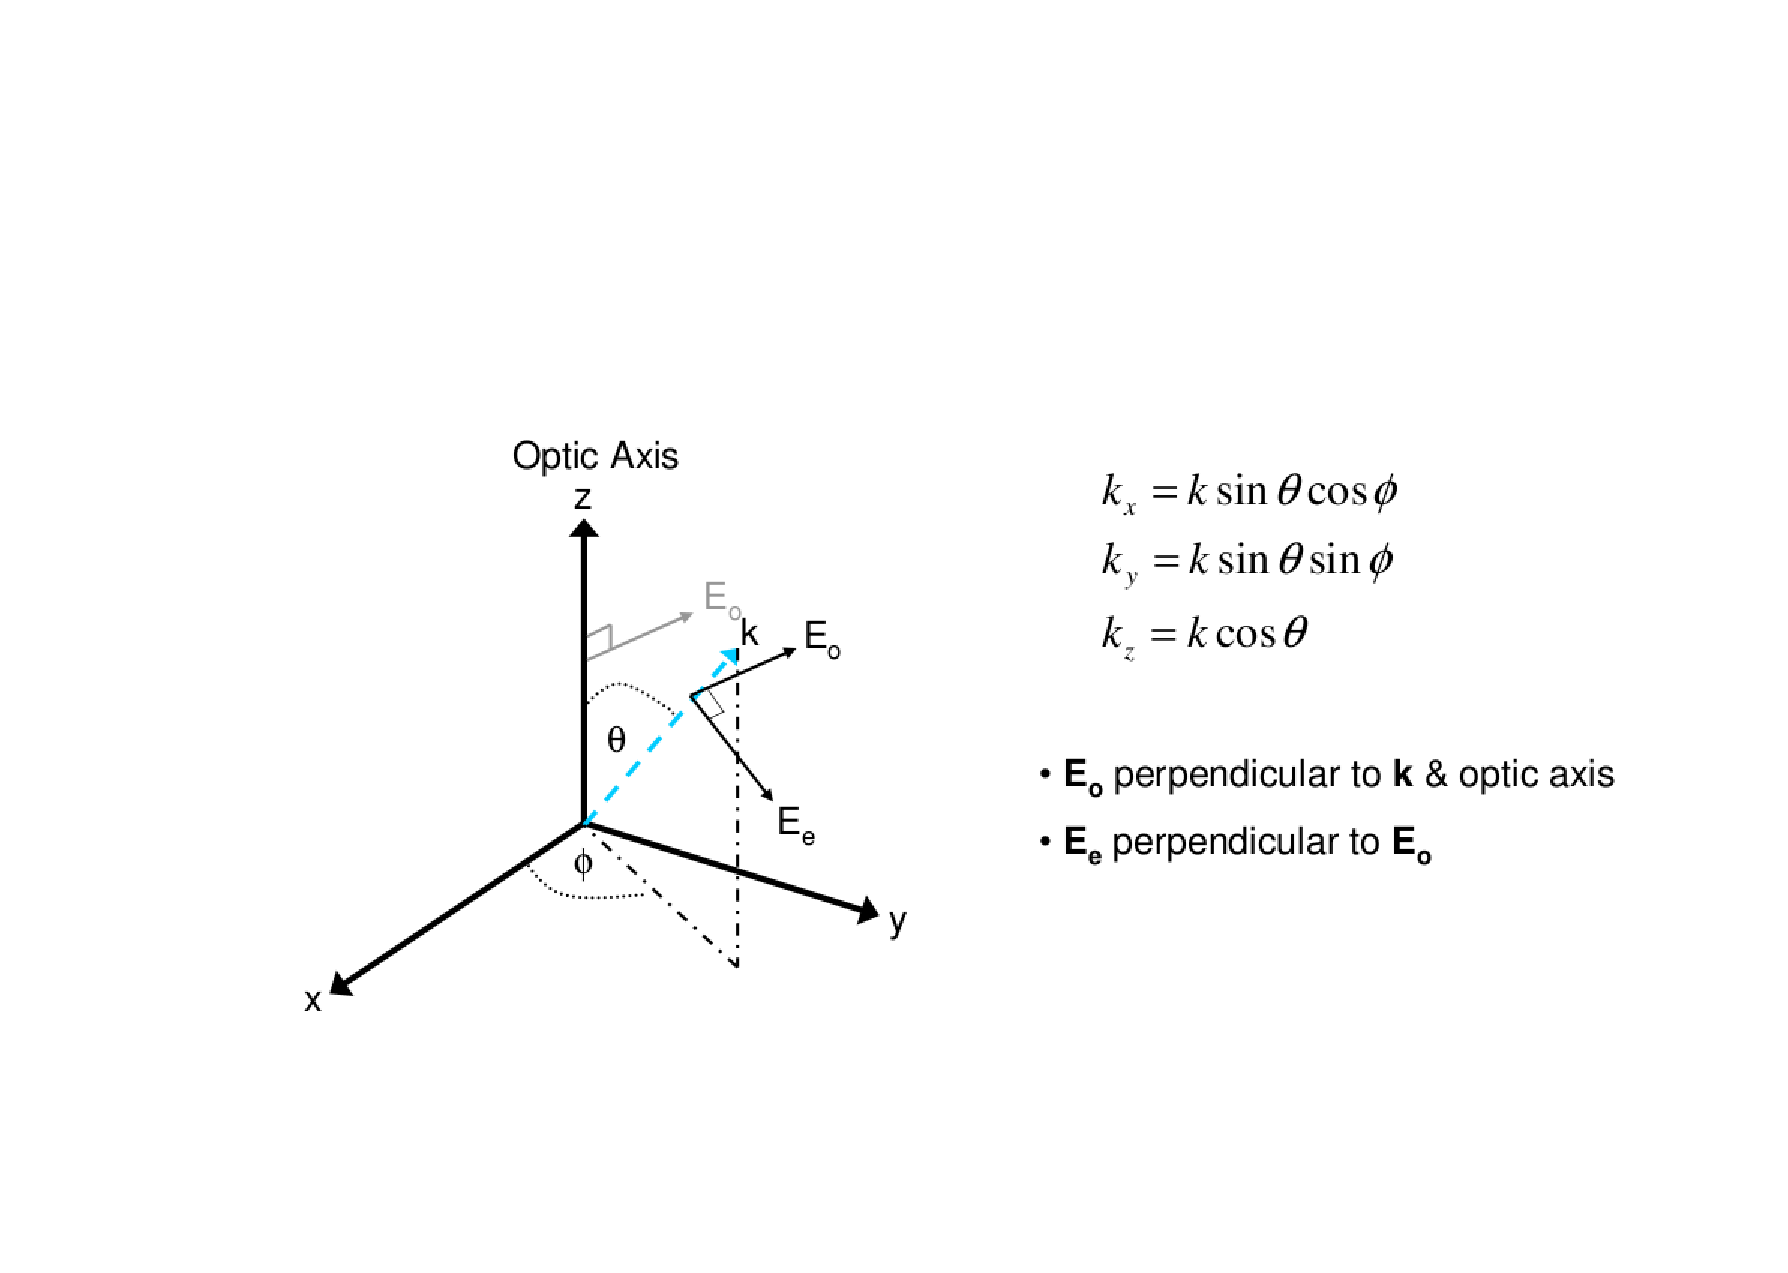
\includegraphics[scale=0.5]{bi.eps}
\end{figure}
For e-ray ($\vec{E_e}$):
\begin{equation*}
\frac{n_o ^2 \omega^2}{c^2} = \left(\frac{n_o}{n_e}\right)^2 (k_x ^2 + k_y ^2) + k_z ^2
\end{equation*}
\begin{equation*}
(k_x ^2 + k_y ^2) (\left(\frac{n_o}{n_e}\right)^2 - 1)E_{x_e} + k_x(\vec{k} \cdot \vec{E_e}) = 0
\end{equation*}
\begin{equation*}
(k_x ^2 + k_y ^2) (\left(\frac{n_o}{n_e}\right)^2 - 1)E_{y_e} + k_y(\vec{k} \cdot \vec{E_e}) = 0
\end{equation*}
\begin{equation*}
k_z ^2 (\left(\frac{n_o}{n_e}\right)^2 - 1)E_{z_e} + k_z(\vec{k} \cdot \vec{E_e}) = 0
\end{equation*}
\begin{equation*}
\frac{E_{x_e}}{E_{y_e}} = \frac{k_x}{k_y} = \cos{\phi}
\end{equation*}
\begin{equation*}
\frac{E_{z_e}}{E_{x_e}} = -\left(\frac{n_o}{n_e}\right)^2 \frac{k_x ^2 + k_y ^2}{k_x k_z} = -\frac{n_o ^2}{n_e ^2}\frac{\tan{\theta}}{\tan{\phi}}
\end{equation*}
\begin{equation}\boxed{
\vec{E_e} = \begin{pmatrix}
1\\
\tan{\phi}\\
-\left(\frac{n_o}{n_e}\right)^2 \frac{\tan{\theta}}{\tan{\phi}}
\end{pmatrix} |E_e|
}\end{equation}
\begin{itemize}
\item[(i)] \begin{equation*}
\vec{E_o}\vec{E_e} = 1 - \frac{k_x}{k_y}\frac{k_y}{k_x} + 0 = 0
\end{equation*}
$\Rightarrow \vec{E_o}$ and $\vec{E_e}$ are perpendicular
\item[(ii)] \begin{equation*}
\vec{k} \cdot \vec{E_e} \neq 0
\end{equation*}
$\Rightarrow$ not perpendicular.
\end{itemize}

\subsubsection{Double refraction}
Ray direction is given by Poynting vector:
\begin{equation*}
\mu_0 \vec{S} = \vec{E} \times \vec{B}
\end{equation*}
for
\begin{equation*}
\vec{E} = \vec{\tilde{E}} e^{i(\vec{k}\vec{r} - \omega t)}
\end{equation*}
\begin{equation*}
\vec{B} = \vec{\tilde{B}} e^{i(\vec{k}\vec{r} - \omega t)}
\end{equation*}

Faraday's law:
\begin{equation*}
\nabla \vec{E} = - \vec{\dot{B}}
\end{equation*}
\begin{equation*}
i\vec{k} \times \vec{E} = i \omega \vec{B}
\end{equation*}
\begin{equation*}
\vec{B} = \frac{1}{\omega}\vec{k} \times \vec{E_0}
\end{equation*}
\begin{equation*}
\mu_0 \vec{S} = \vec{E} \times \vec{B} = \frac{1}{\omega} (\vec{E} \times (\vec{k} \times \vec{E_0}))
\end{equation*}
\begin{equation*}
\omega \mu_0 \vec{S} = \vec{k}(\vec{E} \cdot \vec{E}) - \vec{E} (\vec{E} \cdot \vec{k})
\end{equation*}
therefore, $\vec{S} \parallel \vec{k}$ \textbf{if and only if} $\vec{E} \cdot \vec{k} = 0$. In other words, if $\cos{\alpha} = 0$, where $\alpha$ is the angle between $\vec{E}$ and $\vec{k}$, i.e.
\begin{equation*}
\cos{\alpha} = \frac{\vec{E} \cdot \vec{k}}{|\vec{E}| |\vec{k}|}
\end{equation*}

For o-ray
\begin{equation*}
\vec{E} \cdot \vec{k} = 0
\end{equation*}
therefore $\cos{\alpha} = 0$, $\Rightarrow \alpha = 90^o$

For e-ray
\begin{equation*}
\vec{E_e} \cdot \vec{k} = |E_{x_e}| \left[k_x ^2 + \frac{k_y ^2}{k_x} - \frac{n_o ^2}{n_e ^2} \frac{(k_x ^2 + k_y ^2)}{k_x}\right] = |k||E_{x_e}| \frac{\sin{\theta}}{\cos{\phi}}\left(1 - \frac{n_o ^2}{n_e ^2} \right)
\end{equation*}
\begin{equation*}
|\vec{k}||\vec{E_{e}}| = |k||E_{x_e}| \left(1 + \tan^2{\phi} + \frac{n_o ^4}{n_e ^2} \frac{\tan^2{\theta}}{\cos{\phi}}\right)^{1/2} = \frac{|\vec{k}||\vec{E_{e}}|}{\cos{\phi}} \left(1 + \frac{n_o ^4}{n_e ^2}\tan^2{\theta} \right)^{1/2}
\end{equation*}
\begin{equation}\boxed{
\cos{\alpha} = \frac{\sin{\theta}\left(1-\frac{n_o ^2}{n_e ^2}\right)}{\sqrt{1+\frac{n_o ^4}{n_e ^2}\tan^2{\theta}}} \neq 0
}\end{equation}
except when $\theta = 0$ or $\theta = 90^o$.

\subsubsection{Polarising beamsplitter}
For total internal reflection, $\theta_i > \theta_r$ where $\theta_i = \sin^{-1}{\frac{n_2}{n_1}}$ (in a birefringent crystal $\theta_i$ will be different for all rays).
\begin{figure}[h!]
\centering
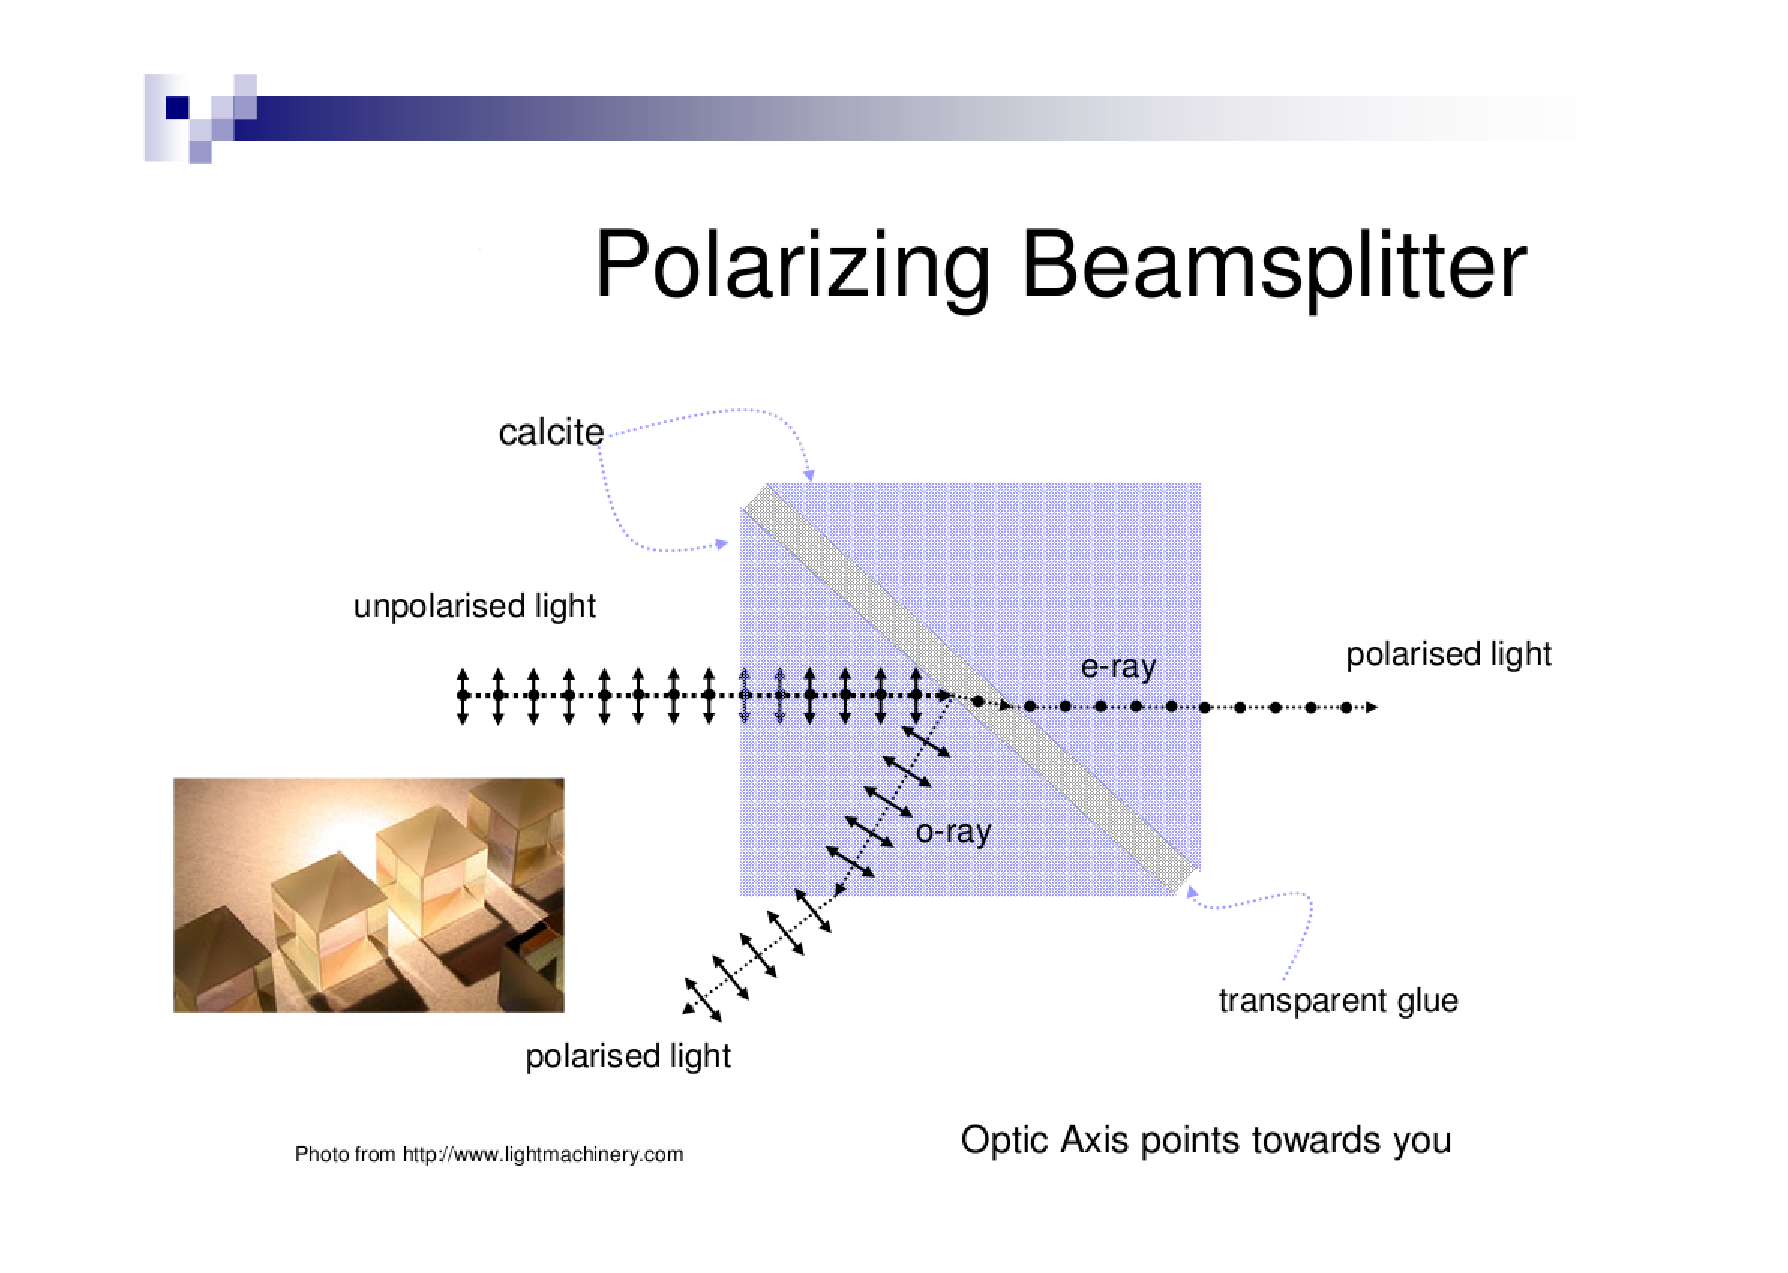
\includegraphics[scale=0.5]{polar.eps}
\end{figure}

For total internal reflection, $\theta_i > \theta_r$ where $\theta_i = \sin^{-1}{\frac{n_2}{n_1}}$ (in a birefringent crystal $\theta_i$ will be different for all rays).

Use this to split unpolarised beam in two orthogonal polarised components.

OA (optical axis) oriented so that rays propagate in same direction until interface ($\theta = 90^o$).

Second piece of calcite ensures e-ray to be parallel to input, aka Slamthompson Polariser or Glan-Foucat Polariser of no cement, just gap.

\begin{itemize}
\item[$\bullet$] $n_o > n_e$ OA is fast;
\item[$\bullet$] $n_e < n_o$ OA is slow.
\end{itemize}
\textbf{Note:} o-ray is \textbf{always} perpendicular to OA.

\subsubsection{Waveplates}
Consider phases of o- and e-rays
\begin{equation*}
\phi_o = k_o z - \omega t
\end{equation*}
\begin{equation*}
\phi_e = k_e z - \omega t
\end{equation*}
where
\begin{equation*}
k_o = \frac{2 \pi n_o}{\lambda}
\end{equation*}
\begin{equation*}
k_e = \frac{2 \pi}{\lambda}n(\theta)
\end{equation*}

Phase difference:
\begin{equation*}
\Delta\phi = \phi_o - \phi_e = (k_o - k_e)z
\end{equation*}

For a crystal of thickness $d$:
\begin{equation*}
\Delta\phi = \frac{2 \pi d}{\lambda}(n_o - n(\theta))
\end{equation*}

If $\theta = 90^o$, so rays do not separate then $n(\theta) = n_e$.
\begin{equation*}
\Delta\phi = \frac{2 \pi d}{\lambda}(n_o - n_e)
\end{equation*}
\begin{itemize}
\item[(i)] Set $d$ so
\begin{equation*}
\Delta\phi = (2m + 1)\pi
\end{equation*}
\begin{equation*}
\Delta\phi = \frac{\lambda}{2}
\end{equation*}
$\Rightarrow$ half wave plate. Flips polarisation direction about optical axis.
\item[(ii)] Set $d$ so
\begin{equation*}
\Delta\phi = (4m + 1)\frac{\pi}{2}
\end{equation*}
\begin{equation*}
\Delta\phi = \frac{\lambda}{4}
\end{equation*}
$\Rightarrow$ quater wave plate. Changes circular polarised light to linear (or vise versa).
\end{itemize}

\subsection{The Faraday effect}
Plane polarisation is rotating as the beam of light passes through a material in the pressure of $B$ field. Rotation angle
\begin{equation*}
\beta = VBd
\end{equation*}
$d$ -- propper distance in material;\\
$B$ -- magnetic field;\\
$V$ -- Verdet constant.\\
\begin{figure}[p!]
\centering
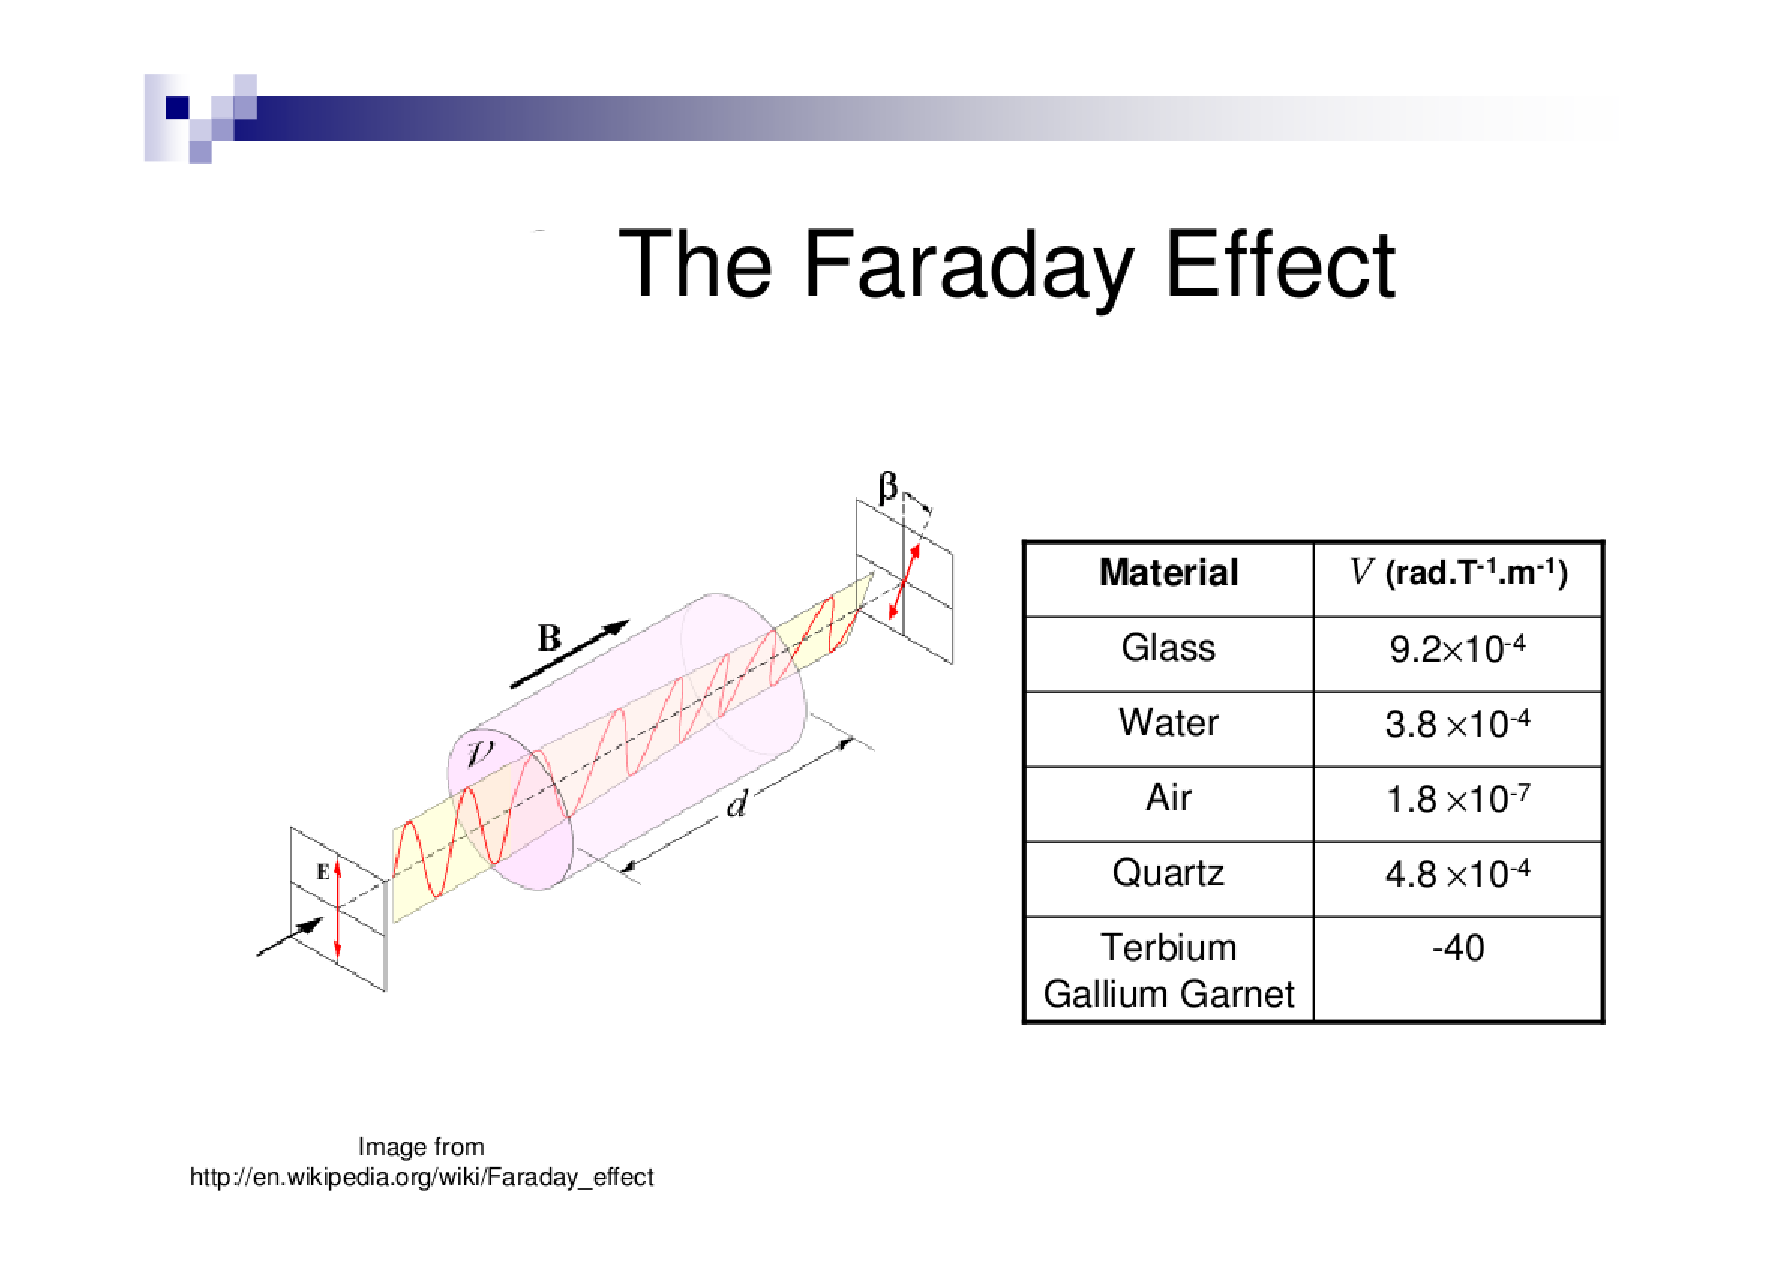
\includegraphics[scale=0.5]{F1.eps}
\end{figure}
\textbf{N.B.:} Direction of rotation depends on sign of $V$ and $B$, \underline{not} on direction of propagation, i.e. for $V>0$.
\begin{figure}[p!]
\centering
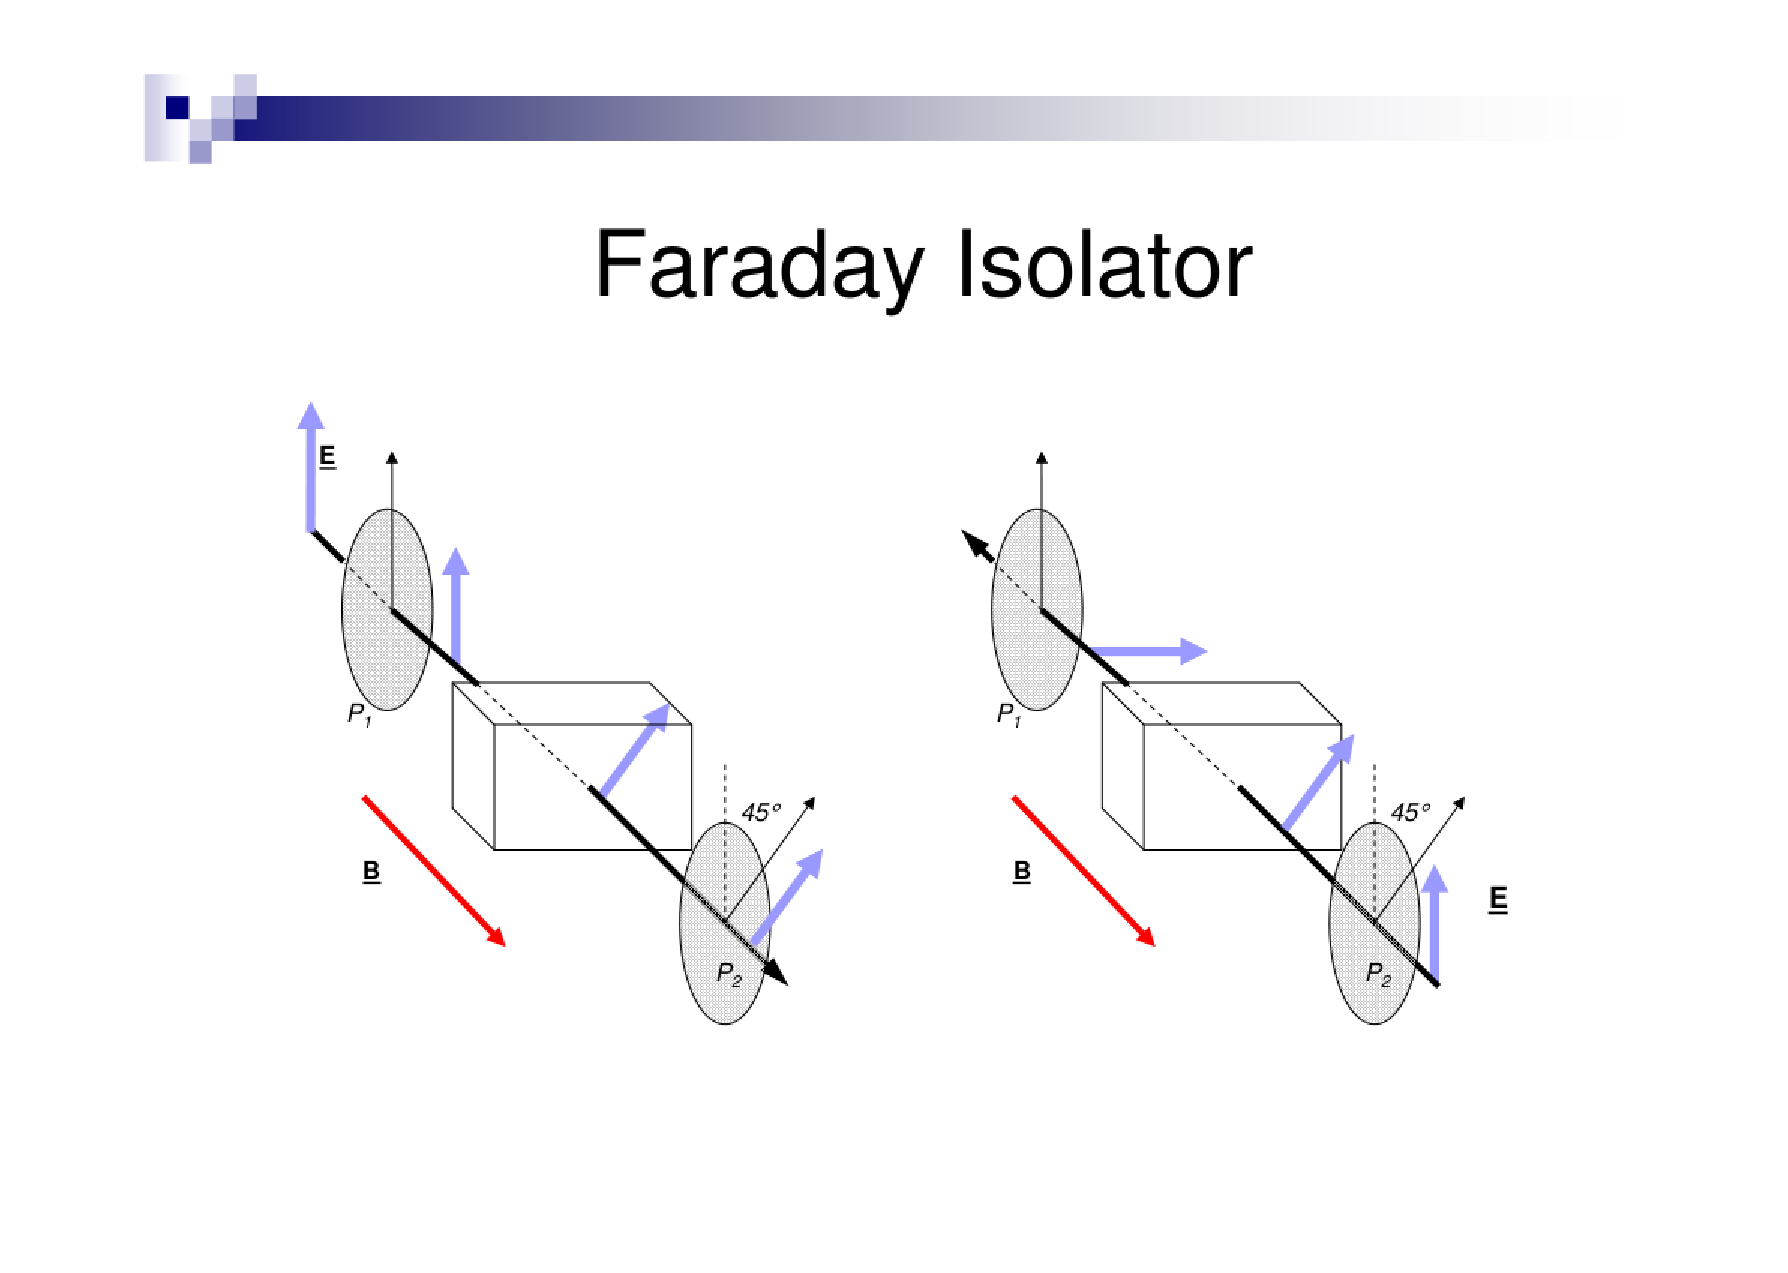
\includegraphics[scale=0.5]{F2.eps}
\end{figure}

\section{Interference}
\subsection{Conditions of interference}
Consider a superposition of two plane waves:
\begin{equation*}
\vec{E} = \vec{E_1}e^{i(\vec{k_1}\vec{r} - \omega_1 t +\phi_1)} + \vec{E_2}e^{i(\vec{k_2}\vec{r} - \omega_2 t +\phi_2)}
\end{equation*}
but we observe
\begin{equation*}
I = \left\langle \vec{E}\vec{E^{*}}\right\rangle \frac{1}{2 \eta}
\end{equation*}
\begin{equation*}
EE^{*} = E_1 ^2 + E_2 ^2 + 2 \vec{E_1} \vec{E_2} \cos{[(\vec{k_1} - \vec{k_2})\vec{r} - (\omega_1 - \omega_2)t + (\phi_1 - \phi_2)]}
\end{equation*}

$\vec{E_1} \vec{E_2} = 0$, if waves are orthogonally polarised, $\Rightarrow$

Condition $1$: $\vec{E_1} \vec{E_2} \neq 0$.

Call
\begin{equation*}
f(t) = \cos{[\Delta \vec{k}\vec{r} - \Delta \omega t + \Delta \phi]}
\end{equation*}
\begin{equation*}
f(t) = \cos{[\Delta \vec{k}\vec{r} + \Delta \phi]} \cos{[\Delta \omega t]} + \sin{[\Delta \vec{k}\vec{r} + \Delta \phi]} \sin{[\Delta \omega t]}
\end{equation*}
\begin{equation*}
\left\langle EE^* \right\rangle = E_1 ^2 + E_2 ^2 + 2\vec+{E_1} \vec{E_2} \left\langle f(t) \right\rangle
\end{equation*}
but
\begin{equation*}
\left\langle sin{(\omega t)} \right\rangle = \left\langle cos{(\omega t)} \right\rangle = 0
\end{equation*}
for $T << \omega^{-1}$ ($T$ is averaging time, not period), therefore
\begin{equation*}
\left\langle f(t) \right\rangle = 0
\end{equation*}
unless $\Delta \omega$ is small comparing to $t \Rightarrow$
\begin{equation*}
\omega_1 - \omega_2 \approx 0
\end{equation*}

So that frequences have to be close together.

Condition $2$: $\omega_1 \approx \omega_2$.

If $\omega_1 \approx \omega_2$, then
\begin{equation*}
\cos{(\Delta \omega t)} = 1
\end{equation*}
and
\begin{equation*}
\sin{(\Delta \omega t)} = 0
\end{equation*}
therefore
\begin{equation*}
f(t) = \cos{(\Delta \vec{k}\vec{r} + \Delta \phi)}
\end{equation*}

Repeat whole process for $\Delta \phi$:
\begin{equation*}
f(t) = \cos{(\Delta \vec{k}\vec{r})} \cos{(\Delta \phi)} - \sin{(\Delta \vec{k}\vec{r})} \sin{(\Delta \phi)}
\end{equation*}

If
\begin{equation*}
\Delta \phi = g(t)
\end{equation*}
have
\begin{equation*}
\left\langle f(t)\right\rangle = 0
\end{equation*}

Condition $3$: $\Delta \phi \approx const$ over $T$.
\begin{itemize}
\item such beam are called coherent;
\item $\Delta \phi = const$ if teo beams come from the same source;
\item very hard to synchronise independent sources so that $\Delta \phi = const$.
\end{itemize}

Summarise of conditions for interference:
\begin{enumerate}
\item $\vec{E_1} \vec{E_2} \neq 0$ "non-orthogonal polarisation"
\item $\Delta \omega \leq T^{-1}$ "narrow boundary"
\item $\Delta \phi \approx const$ "coherent sources"
\end{enumerate}

\subsection{Coherence}
Coherent waves are waves that maintain constant phase relationship.

\subsubsection{Temporal coherence}
If $\Delta \omega \neq 0$, phase relationship will change over a period of $\Delta \omega^{-1}$.

So for monochromatic light coherence time is defined
\begin{equation}\boxed{
\tau_c = \frac{1}{\Delta \nu}
}\end{equation}
where $\Delta \nu$ is frequency band width.

Coherence length:
\begin{equation}\boxed{
l_c = c \tau_c
}\end{equation}
"characteristic path length difference for two beams over which interference can be observed".
\subsubsection{Spatial Coherence}
\begin{itemize}
\item Spatially coherence beams maintain fixed phase relationship along a wavefront.
\item Important if different paths of a wavefront are to interfer.
\item Such as in \textit{wavefront division interference}.
\item Not so important for \textit{amplitude division interference}.
\end{itemize}

\subsubsection{Fringes and Fringe visibility}
For parallel polarised, monochromatic coherent beams
\begin{equation}\boxed{
I = I_1 + I_2 + 2 \sqrt{I_1I_2}\cos{\delta}
}\end{equation}
where
\begin{equation*}
\delta = (\vec{k_1} - \vec{k_2})\vec{r} + \Delta \phi
\end{equation*}

If $\cos{\delta} > 0 \Rightarrow$ constructive interference.

If $\cos{\delta} < 0 \Rightarrow$ distructive interference.\\
$\Rightarrow$ series of bright + light bands $\Rightarrow$ "interference fringes"

If 
\begin{equation*}
I_1 = I_2 = I_0
\end{equation*}
then
\begin{equation}\boxed{
I = 2I_0 + 2I_0 \cos{\delta} = 4I_0 \cos^2{\frac{\delta}{2}}
}\end{equation}

If
\begin{equation*}
I_1 \neq I_2
\end{equation*}
$\Rightarrow$ fringe visibility
\begin{equation}\boxed{
V = \frac{I_{max} - I_{min}}{I_{max} + I_{min}} = \frac{2\sqrt{I_1I_2}}{I_1 + I_2}
}\end{equation}

Fringe visibility is sometimes called "contrast", "modulation", etc.

\subsection{Wavefront division interference}
\subsubsection{Young's Slits}
Young used a candle-broadband, unpolarised, incoherent.

How did it worked?

\begin{figure}[p!]
\centering
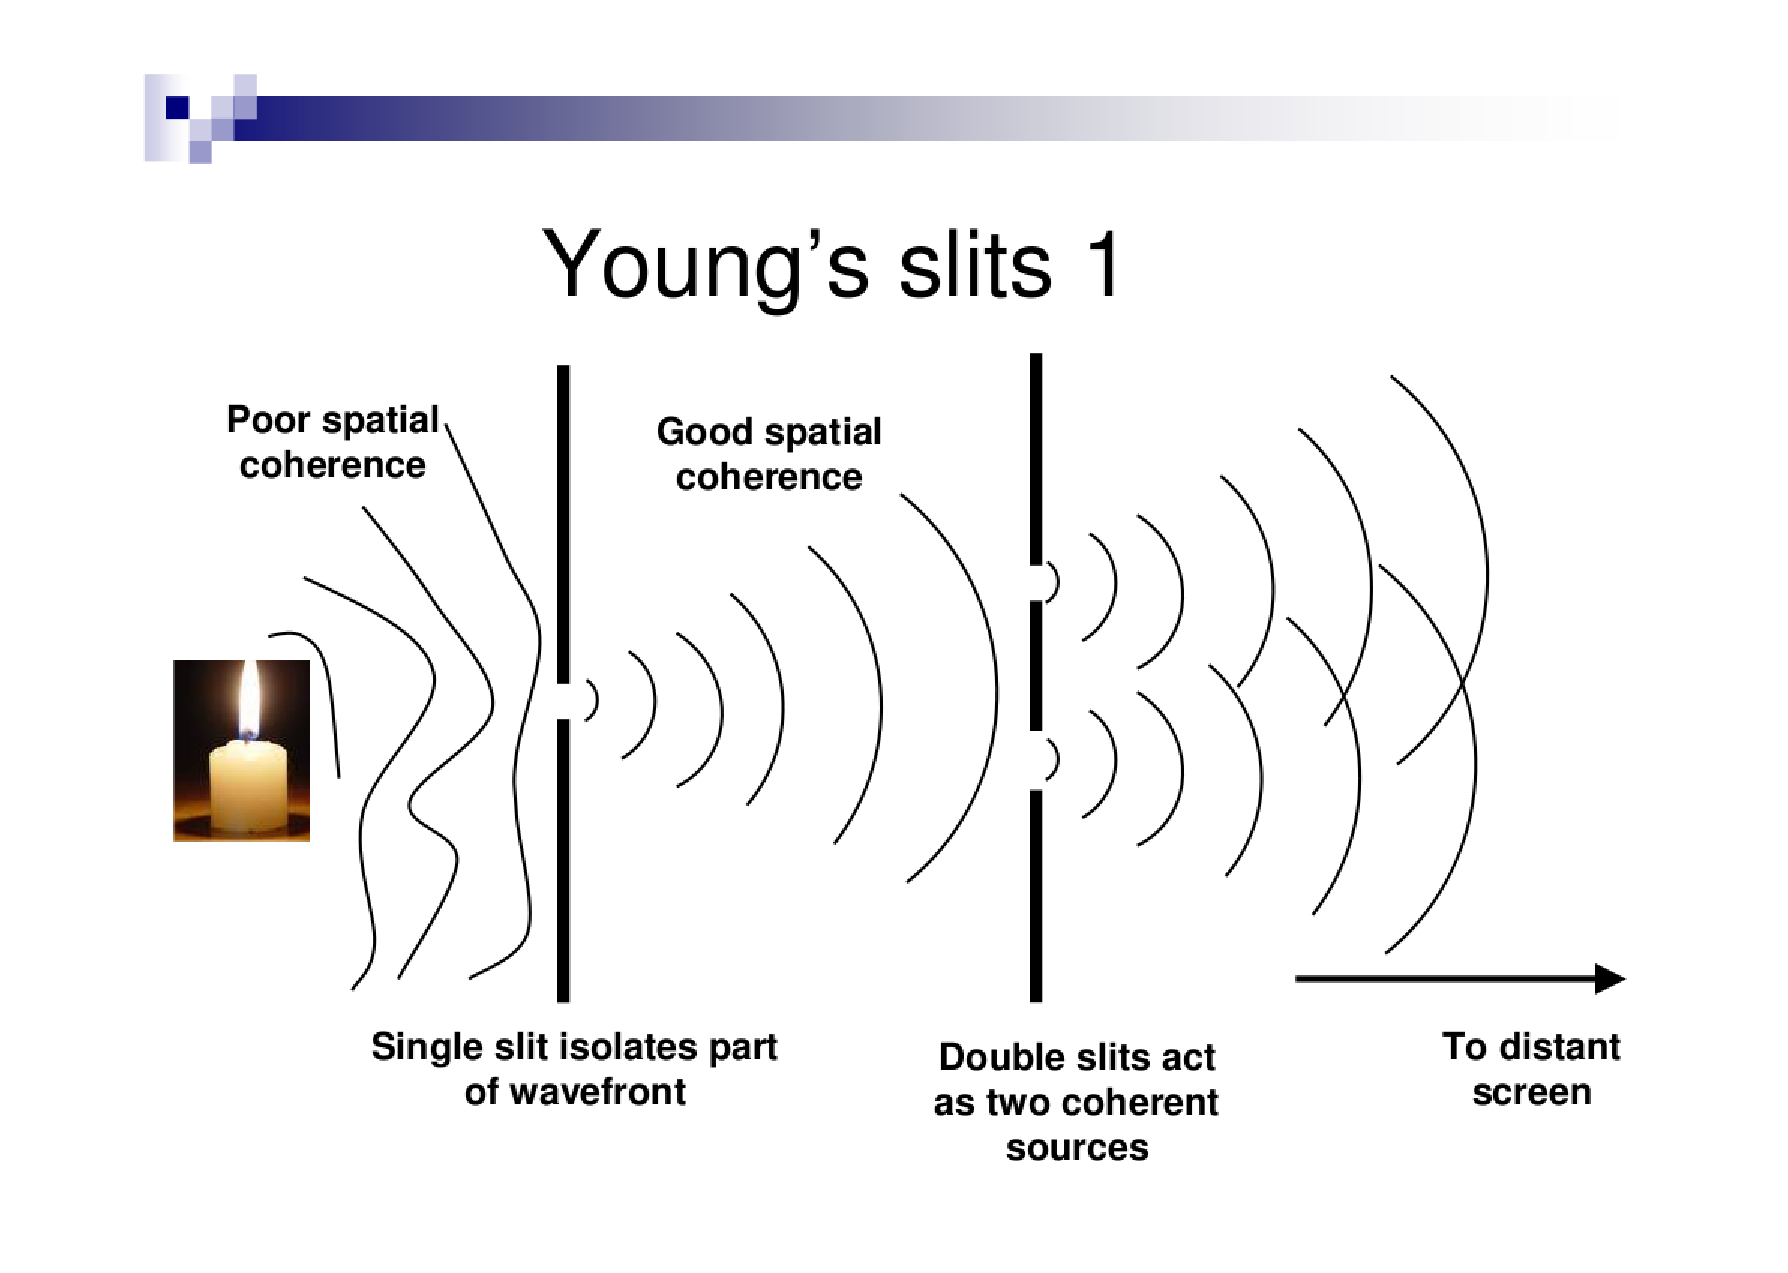
\includegraphics[scale=0.5]{Young.eps}
\end{figure}
\begin{figure}[p!]
\centering
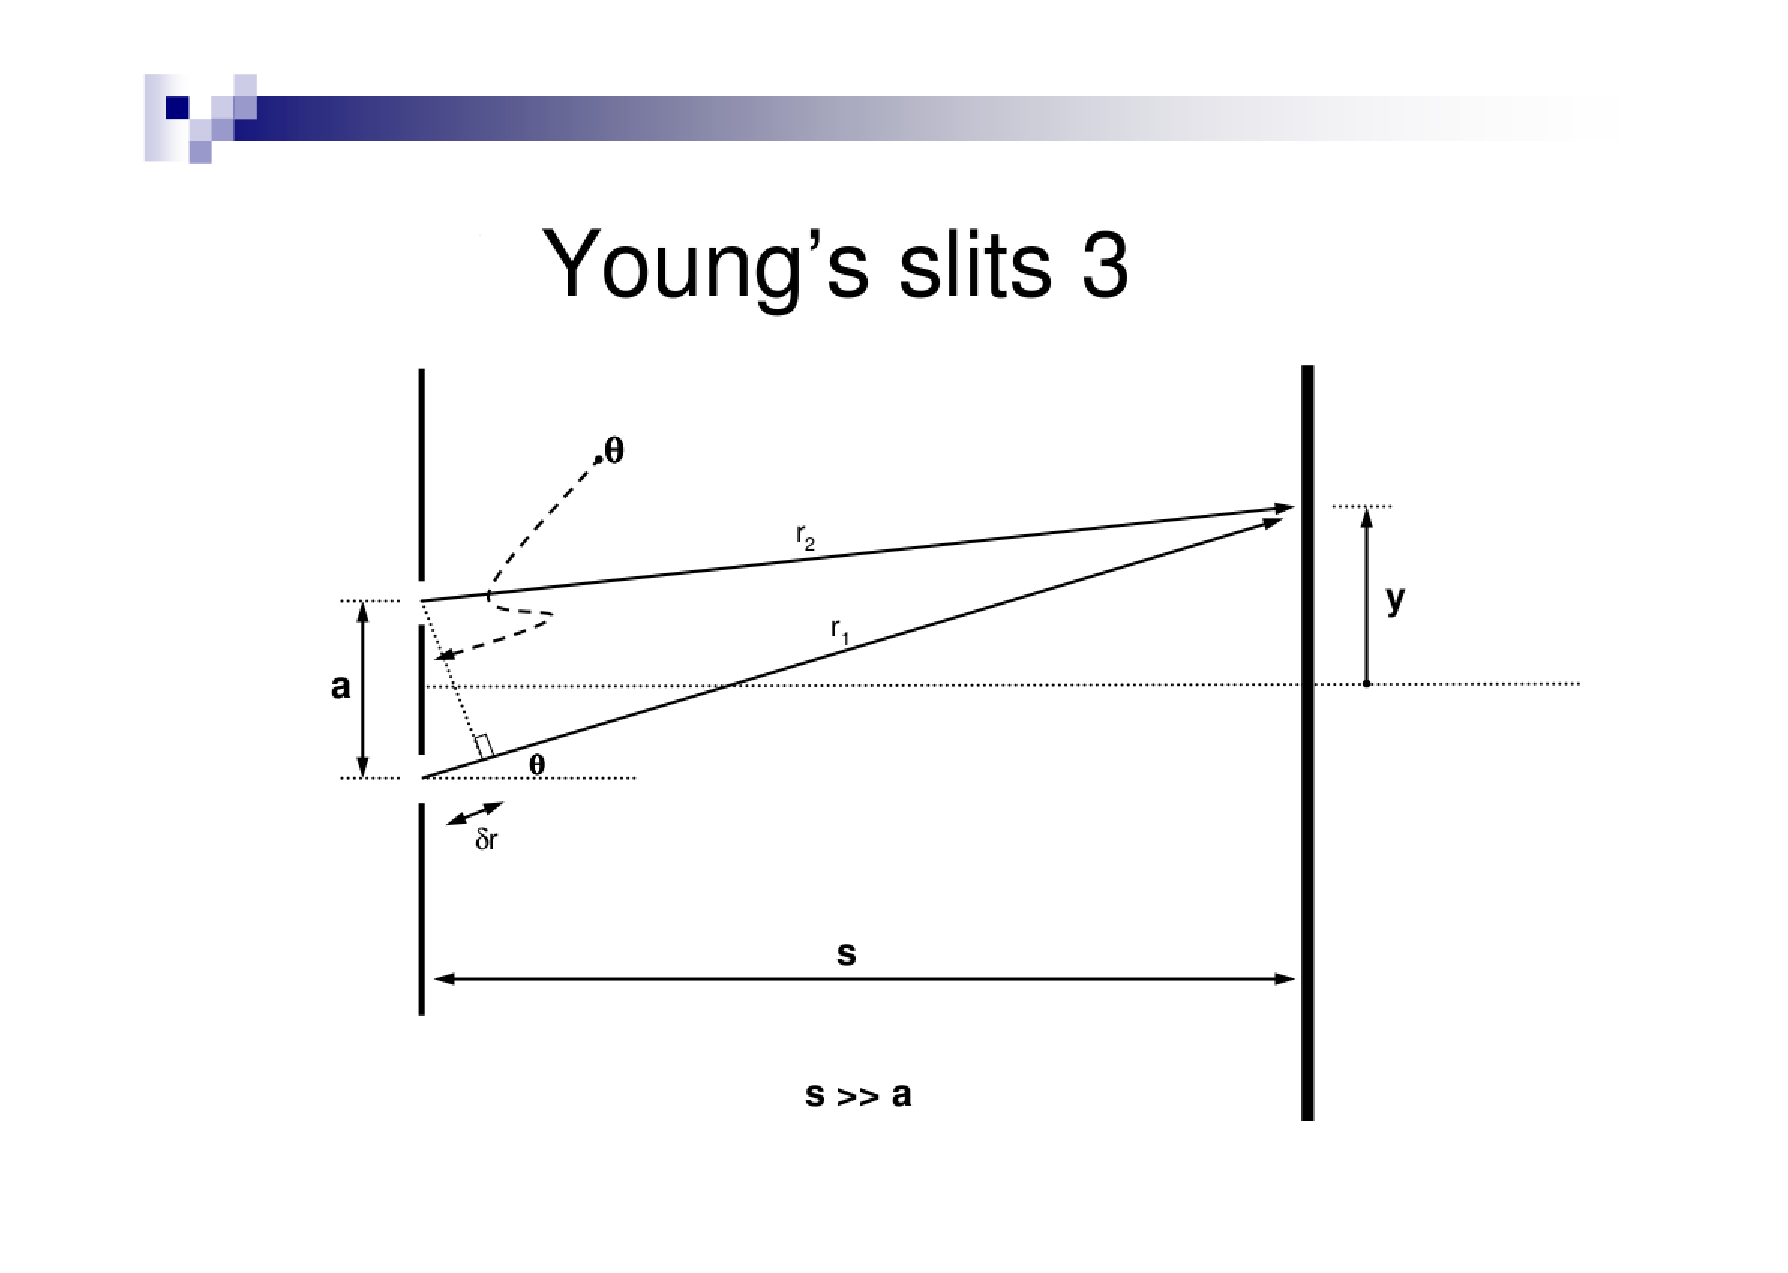
\includegraphics[scale=0.5]{Young2.eps}
\end{figure}

Firs slit ensured great spatial coherence at double slit, therefore slits were coherent sources.

Path length difference (pld) to screen was small, hence
\begin{itemize}
\item instantaneous polarisation source;\
\item pld $<$ coherence light.
\end{itemize}

Slits produce a cylindrical wavefront.
\begin{equation*}
\frac{e^{i(\vec{k}\vec{r} - \omega t)}}{\sqrt{2}}
\end{equation*}
\begin{equation*}
\vec{E} = \vec{E_1}e^{i(\vec{k}\vec{r_1} - \omega_1 t + \phi_1)} + \vec{E_2}e^{i(\vec{k}\vec{r_2} - \omega_2 t + \phi_2)}
\end{equation*}
\begin{equation*}
\vec{E}\vec{E^*} = \frac{E_1 ^2}{r_1} + \frac{E_2 ^2}{r_2} + \frac{2E_1E_2}{\sqrt{r_1r_2}} \cos{k(r_1 - r_2) - \Delta \omega t + \Delta \phi}
\end{equation*}

For coherence somewhere with
\begin{equation*}
l \geq |\vec{r_1} - \vec{r_2}|
\end{equation*}

For $r_1 = r_2 = r$:
\begin{equation*}
\left\langle EE^* \right\rangle = \frac{\left( E_1 ^2 + E_2 ^2 \right) + 2E_1E_2\cos{k(\vec{r_1} - \vec{r_2})}}{r}
\end{equation*}
assume slits are of equal width:
\begin{equation*}
E_1 = E_2
\end{equation*}
\begin{equation*}
I_1 = I_2 = I_0
\end{equation*}
\begin{equation*}
I = \frac{4 I_0}{r}\cos^2{\frac{\delta}{2}}
\end{equation*}
where
\begin{equation*}
\delta = k(\vec{r_1} - \vec{r_2})
\end{equation*}
\begin{equation*}
\delta = k \delta r = ka\sin{\theta} \approx ka\theta \approx ka\frac{y}{s} = \frac{2\pi}{\lambda}a\frac{y}{s}
\end{equation*}
\begin{equation}\boxed{
I = \frac{4I_0}{r}\cos^2{\frac{\pi a y}{\lambda s}}
}\end{equation}

\subsubsection{Lloyd's mirror}
It is actually a variation of Young's slits: two sources are now one source and its reflection.
\begin{figure}[h]
\centering
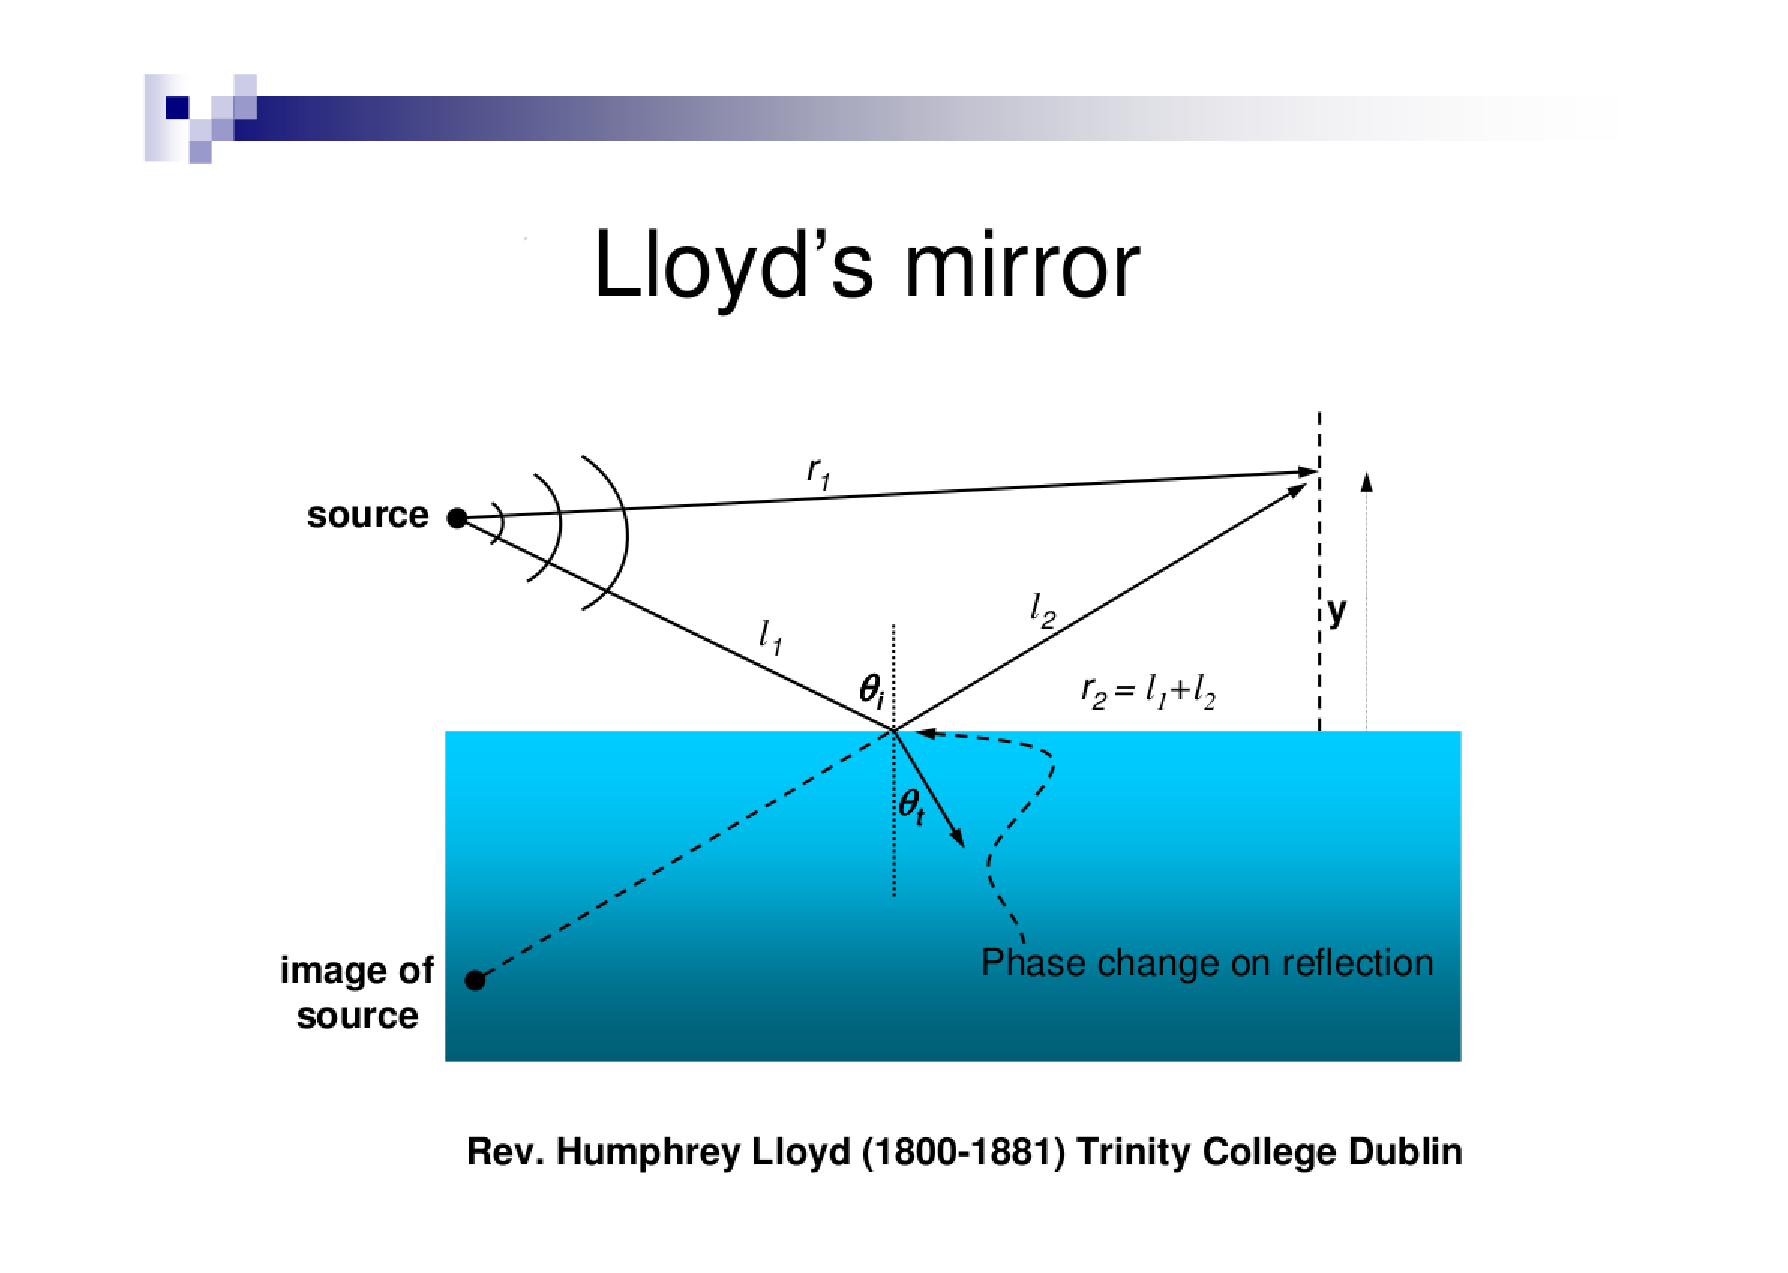
\includegraphics[scale=0.5]{Young3.eps}
\end{figure}

But now ray two undergoes a reflection
\begin{itemize}
\item for s-pol:
\begin{equation*}
r_s = - \frac{\sin{(\theta_i - \theta_t)}}{\sin{(\theta_i - \theta_t)}}
\end{equation*}
\item for p-pol:
\begin{equation*}
r_p = \frac{\tan{(\theta_i - \theta_t)}}{\tan{(\theta_i - \theta_t)}}
\end{equation*}
\end{itemize}

For $\theta_i \leq 90^o$ and $n_i < n_t$, then $r_s < 0$ and $r_p < 0$ therefore $E_i$ and $E_t$ are of opposite sign for both polarisations, i.e. ray undergoes $\pi$ phase change and reflection (as $e^{i\pi} = 1$).
\begin{equation*}
\delta = k(r_1 - r_2) + \pi
\end{equation*}
\begin{equation*}
I = \frac{4I_0}{r}\cos^2{\left(\frac{\pi ay}{\lambda s} + \frac{\pi}{2}\right)}
\end{equation*}
\begin{equation}\boxed{
I = \frac{4I_0}{r}\sin^2{\left(\frac{\pi ay}{\lambda s}\right)}
}\end{equation}

\subsubsection{Multiple slits}
Path lengths:
\begin{figure}[h]
\centering
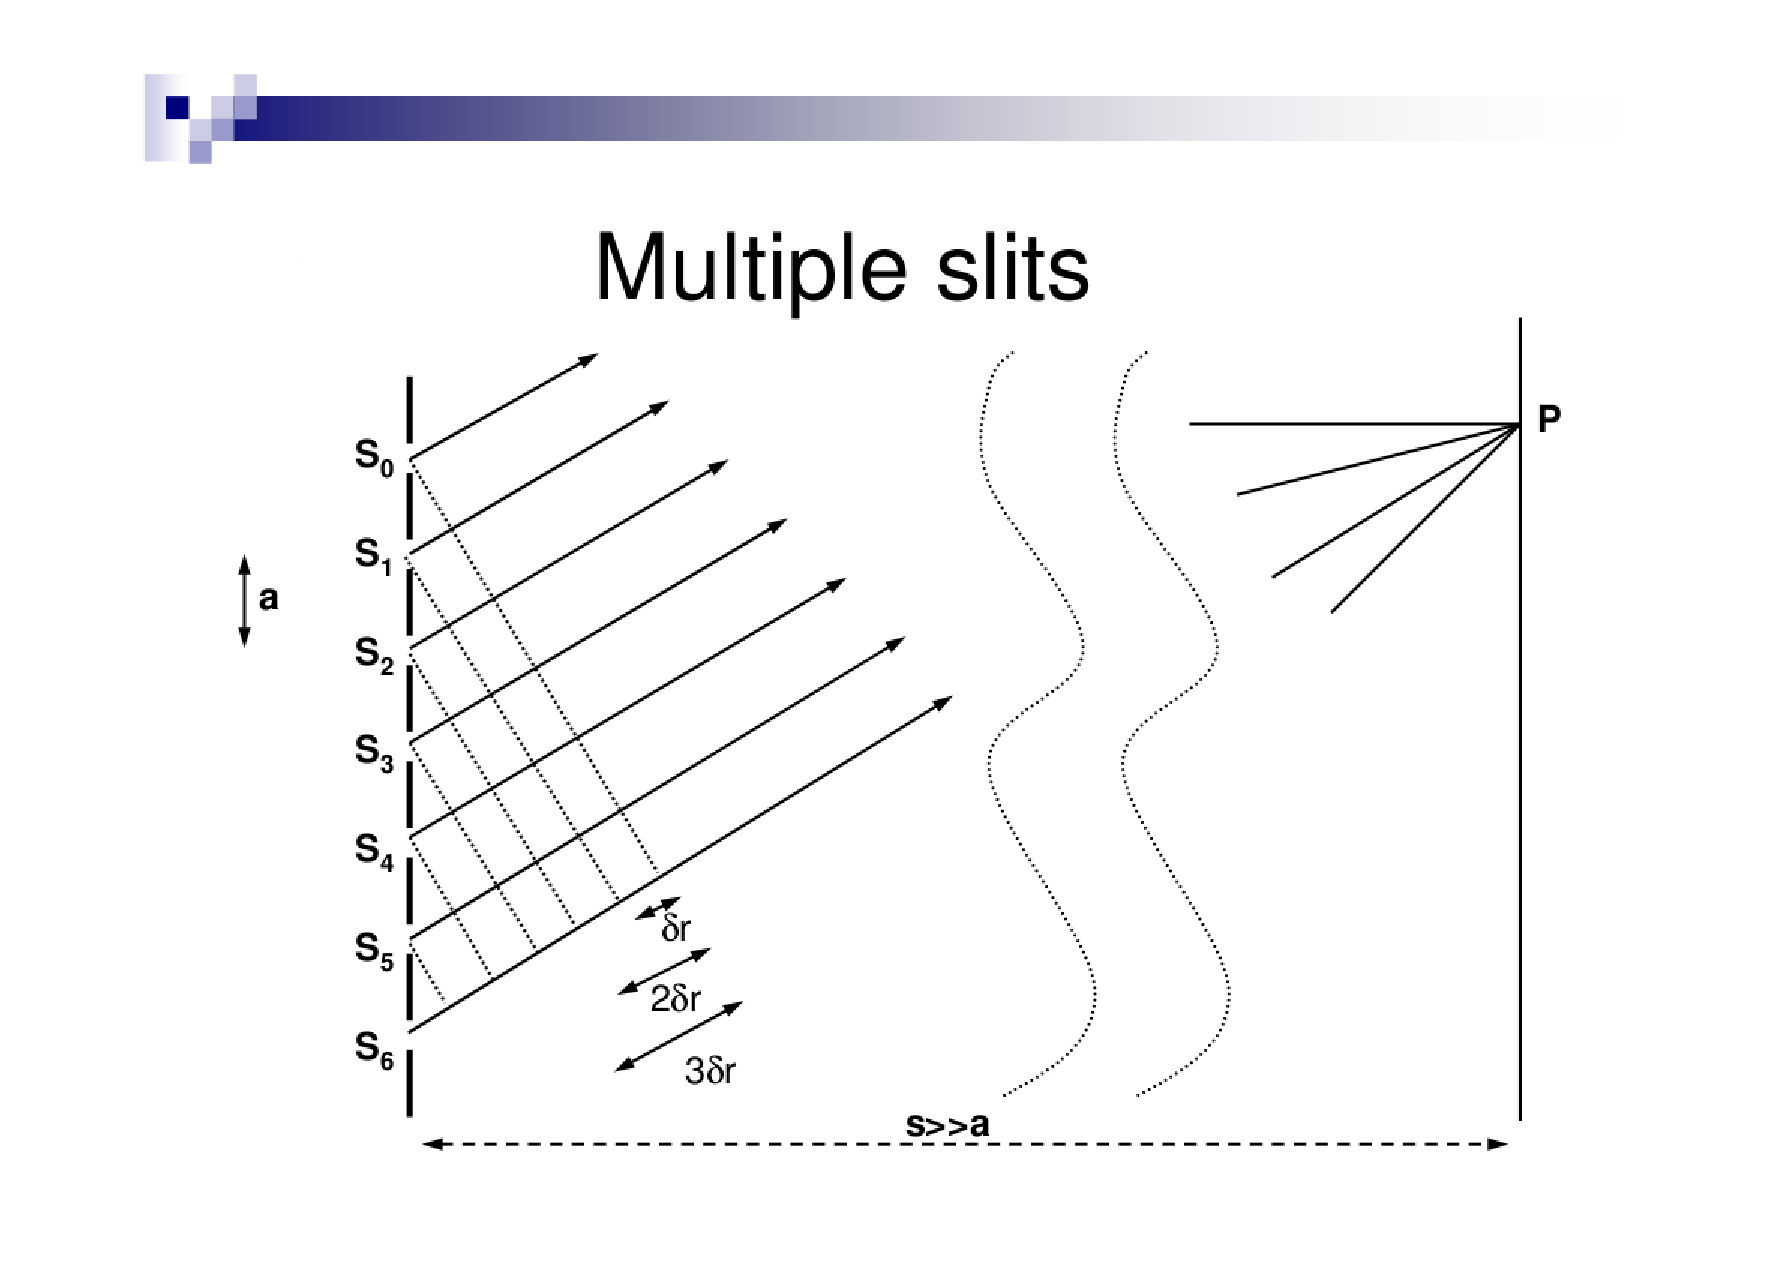
\includegraphics[scale=0.5]{Young4.eps}
\end{figure}
\begin{eqnarray*}
s_0 \rightarrow P &=& r_1 \\
s_1 \rightarrow P &=& r_1 + \delta r \\
s_2 \rightarrow P &=& r_1 + 2 \delta r \\
\vdots \\
s_{N-1} \rightarrow P &=& r_1 + (N-1) \delta r \\
\end{eqnarray*}
therefore $n^{th}$ path length,
\begin{equation*}
r_n = r_1 + n \delta r
\end{equation*}
but
\begin{equation*}
\delta r = a \theta
\end{equation*}
\begin{equation*}
r_n = r_1 + na \theta
\end{equation*}
for $s>>a$
\begin{equation*}
r_n = s + na \theta
\end{equation*}

Field from $n^{th}$ slit at $P$:
\begin{equation*}
E = E_0 \sum^{N-1}_{n=0} \frac{e^{ekr_n}}{\sqrt{r_n}}
\end{equation*}
for changes $\lambda$-scale
\begin{equation*}
r_n ^2 \approx s
\end{equation*}
in denominator.
\begin{flalign*}
E & = \frac{E_0}{\sqrt{s}} \sum_{n=0}^{N-1}e^{ik(s + na \theta)} \\
 & = \frac{E_0}{\sqrt{s}}e^{iks}\sum_{n=0}^{N-1}e^{ikna \theta} \\
 & = \frac{E_0}{\sqrt{s}}e^{iks} \frac{1 - e^{ikNa \theta}}{1 - e^{ika \theta}} \\
 & = \frac{E_0}{\sqrt{s}}e^{iks} \frac{e^{\frac{ikNa \theta}{2}} - e^{-\frac{ikNa \theta}{2}}}{e^{\frac{ika \theta}{2}} - e^{-\frac{ika \theta}{2}}}\\
\end{flalign*}
\begin{equation}\boxed{
I = \frac{I_0}{s} \frac{\sin^2{\frac{kaN \theta}{2}}}{\frac{ka \theta}{2}}
}\end{equation}

\subsection{Amplitude division interference}
\subsubsection{The Michelson interferometer}
\begin{figure}[h]
\centering
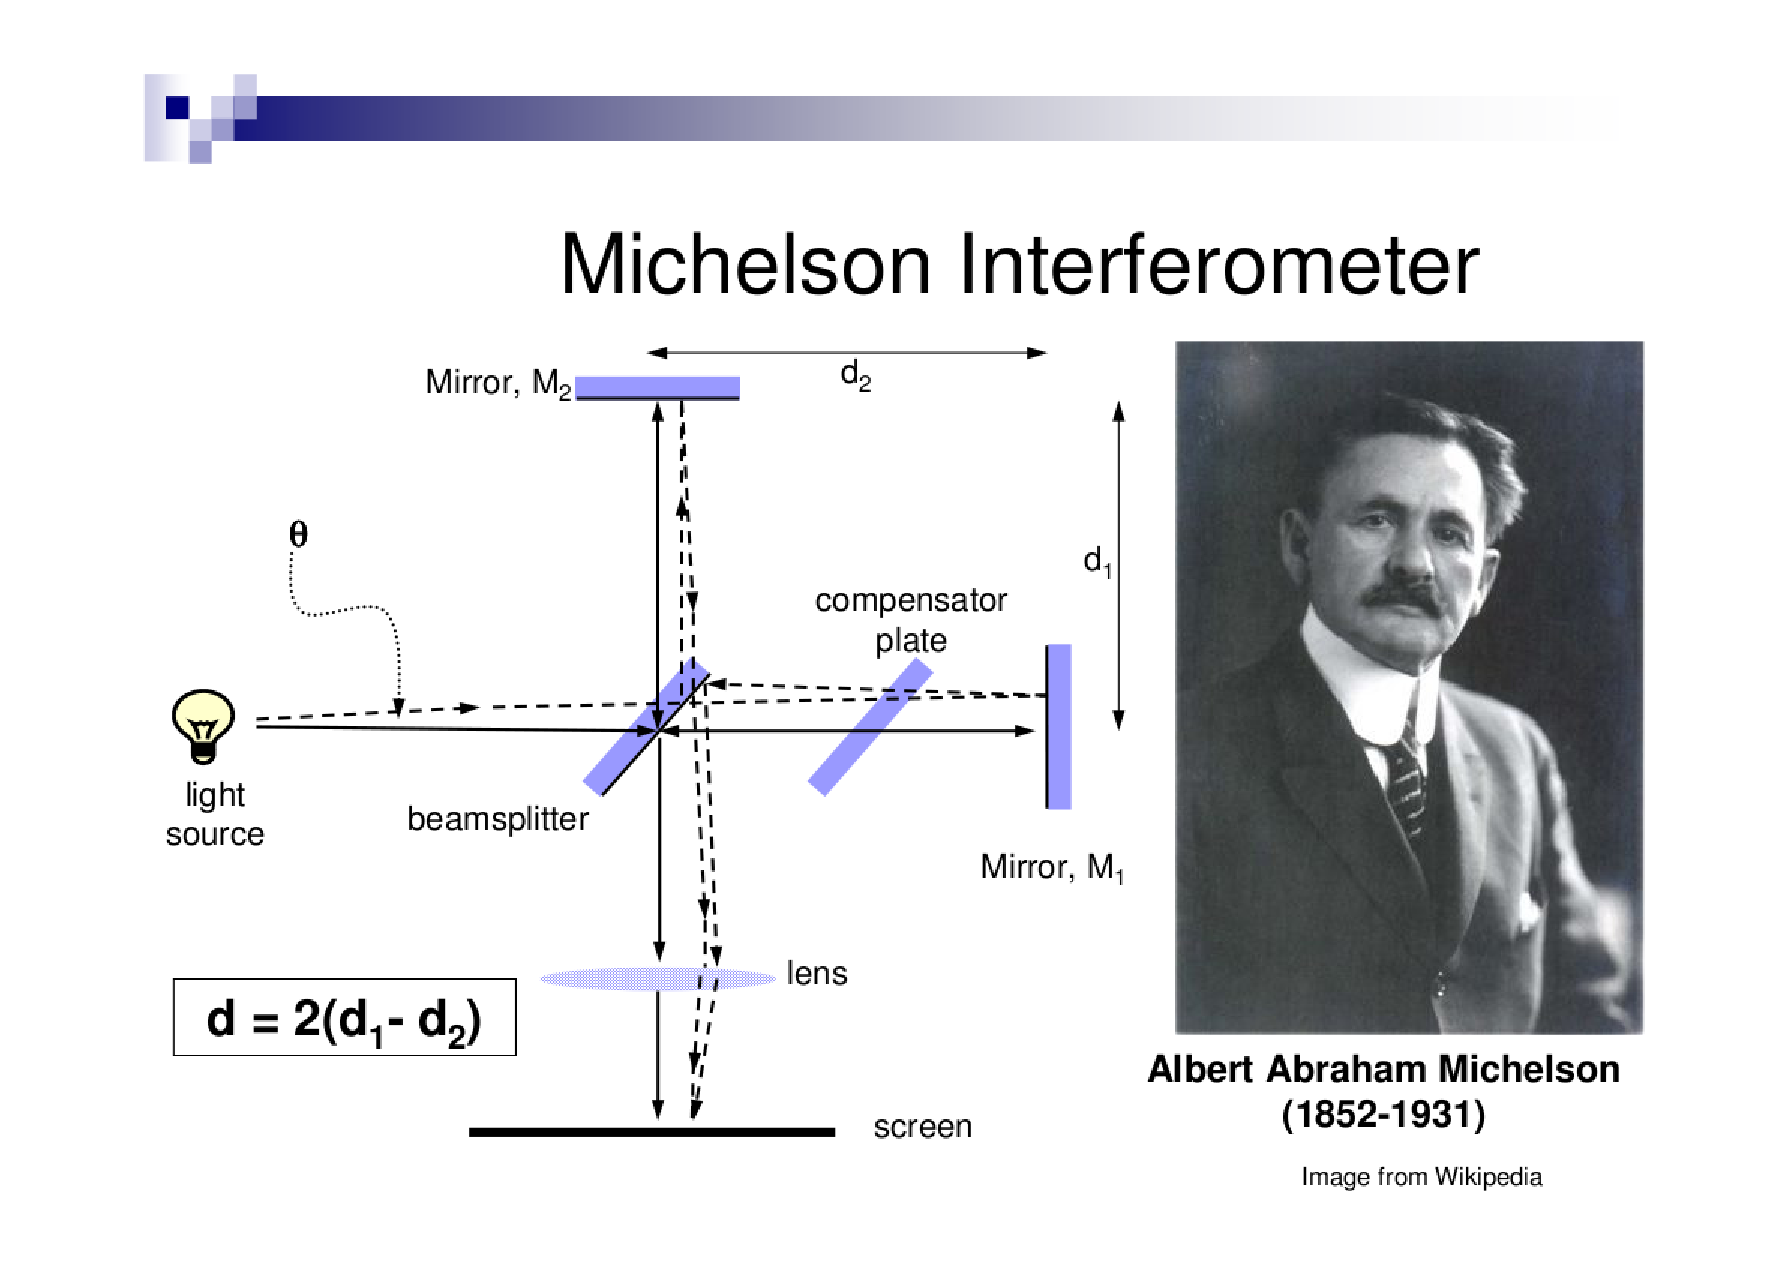
\includegraphics[scale=0.5]{mik.eps}
\end{figure}
P.l.d.
\begin{equation*}
\delta r = d \cos{\theta}
\end{equation*}

Phase difference
\begin{equation*}
\delta = k \delta r + \phi
\end{equation*}
-- one beam undergoes more reflection.

Bright fringes occur when
\begin{equation*}
\delta = 2\pi m
\end{equation*}
\begin{equation*}
kd\cos{\theta_m} + \phi = 2\pi m
\end{equation*}
$\theta_m$ -- angle when bright fringe occurs.
\begin{equation*}
\frac{2\pi d}{\lambda}\cos{\theta_m} = 2\pi m - \phi
\end{equation*}
\begin{equation*}
d\cos{\theta_m} = m\lambda - \delta \lambda
\end{equation*}
\begin{equation*}
\delta \lambda = \frac{\lambda \phi}{2 \pi}
\end{equation*}
\begin{itemize}
\item Fringes are circular if Michelson is well aligned.
\item Central fringe corresponds to the greatest value of $m$.
\end{itemize}

For central fringe, $\theta = 0$.
\begin{equation*}
d = m_0\lambda - \delta \lambda
\end{equation*}

For $p^{th}$ fringe from centre:
\begin{equation*}
d\cos{\theta_p} = (m_0 - p)\lambda - \delta \lambda
\end{equation*}
combine $\Rightarrow$
\begin{equation*}
p \lambda = d(1 - \cos{\theta_p})
\end{equation*}
for small $\theta$:
\begin{equation*}
\cos{\theta} = 1 - \frac{\theta^2}{2}
\end{equation*}
\begin{equation}\boxed{
\theta_p = \sqrt{\frac{2p\lambda}{d}}
}\end{equation}

\subsubsection{The Micelson interferometer as a spectrograph. Fourier Transform Spectroscopy}
Consider only $\theta = 0$.
\begin{itemize}
\item[(i)] For quasimonochromatic light: field of the direction
\begin{equation*}
E = E_0 e^{ik2d_1} + E_0 e^{ik2d_2}
\end{equation*}
\begin{equation*}
I = 2I_0 [1 + \cos{kd}]
\end{equation*}
where
\begin{equation*}
d = 2(d_1 - d_2)
\end{equation*}
\item[(ii)] For polychromatic light:

Now let
\begin{equation*}
I_0 = \int_0^\infty I(k)dk
\end{equation*}
here we're considering only one direction ($\theta = 0$), so $k$ can be a scalar, therefore total intensity at detector:
\begin{equation*}
I(d) = 2 \int_0 ^\infty I(k) (1 + \cos{kd})dk = 2 I_0 + 2 \int_0 ^\infty I(k)\cos{kd}dk
\end{equation*}
but
\begin{equation*}
F_c ^{-1} (I(k)) = \frac{2}{\pi} \int_0 ^\infty I(k)\cos{kd}dk
\end{equation*}
\begin{equation*}
I(d) = 2I_0 + \pi F_c ^{-1} (I(k))
\end{equation*}

So we measure $I(d)$
\begin{equation*}
F_c (const) = 0
\end{equation*}
\begin{equation*}
F_c (I(d)) = F_c(2I_0) + \pi F_c(F_c ^{-1} (I(k))) = \pi I(k)
\end{equation*}
\end{itemize}

\subsubsection{Thin film}
Reflectivity of dielectric interfaces is low (e.g. glass-airis about $4\%$).

Rays reflected more than once are negligible.
\begin{figure}[h]
\centering
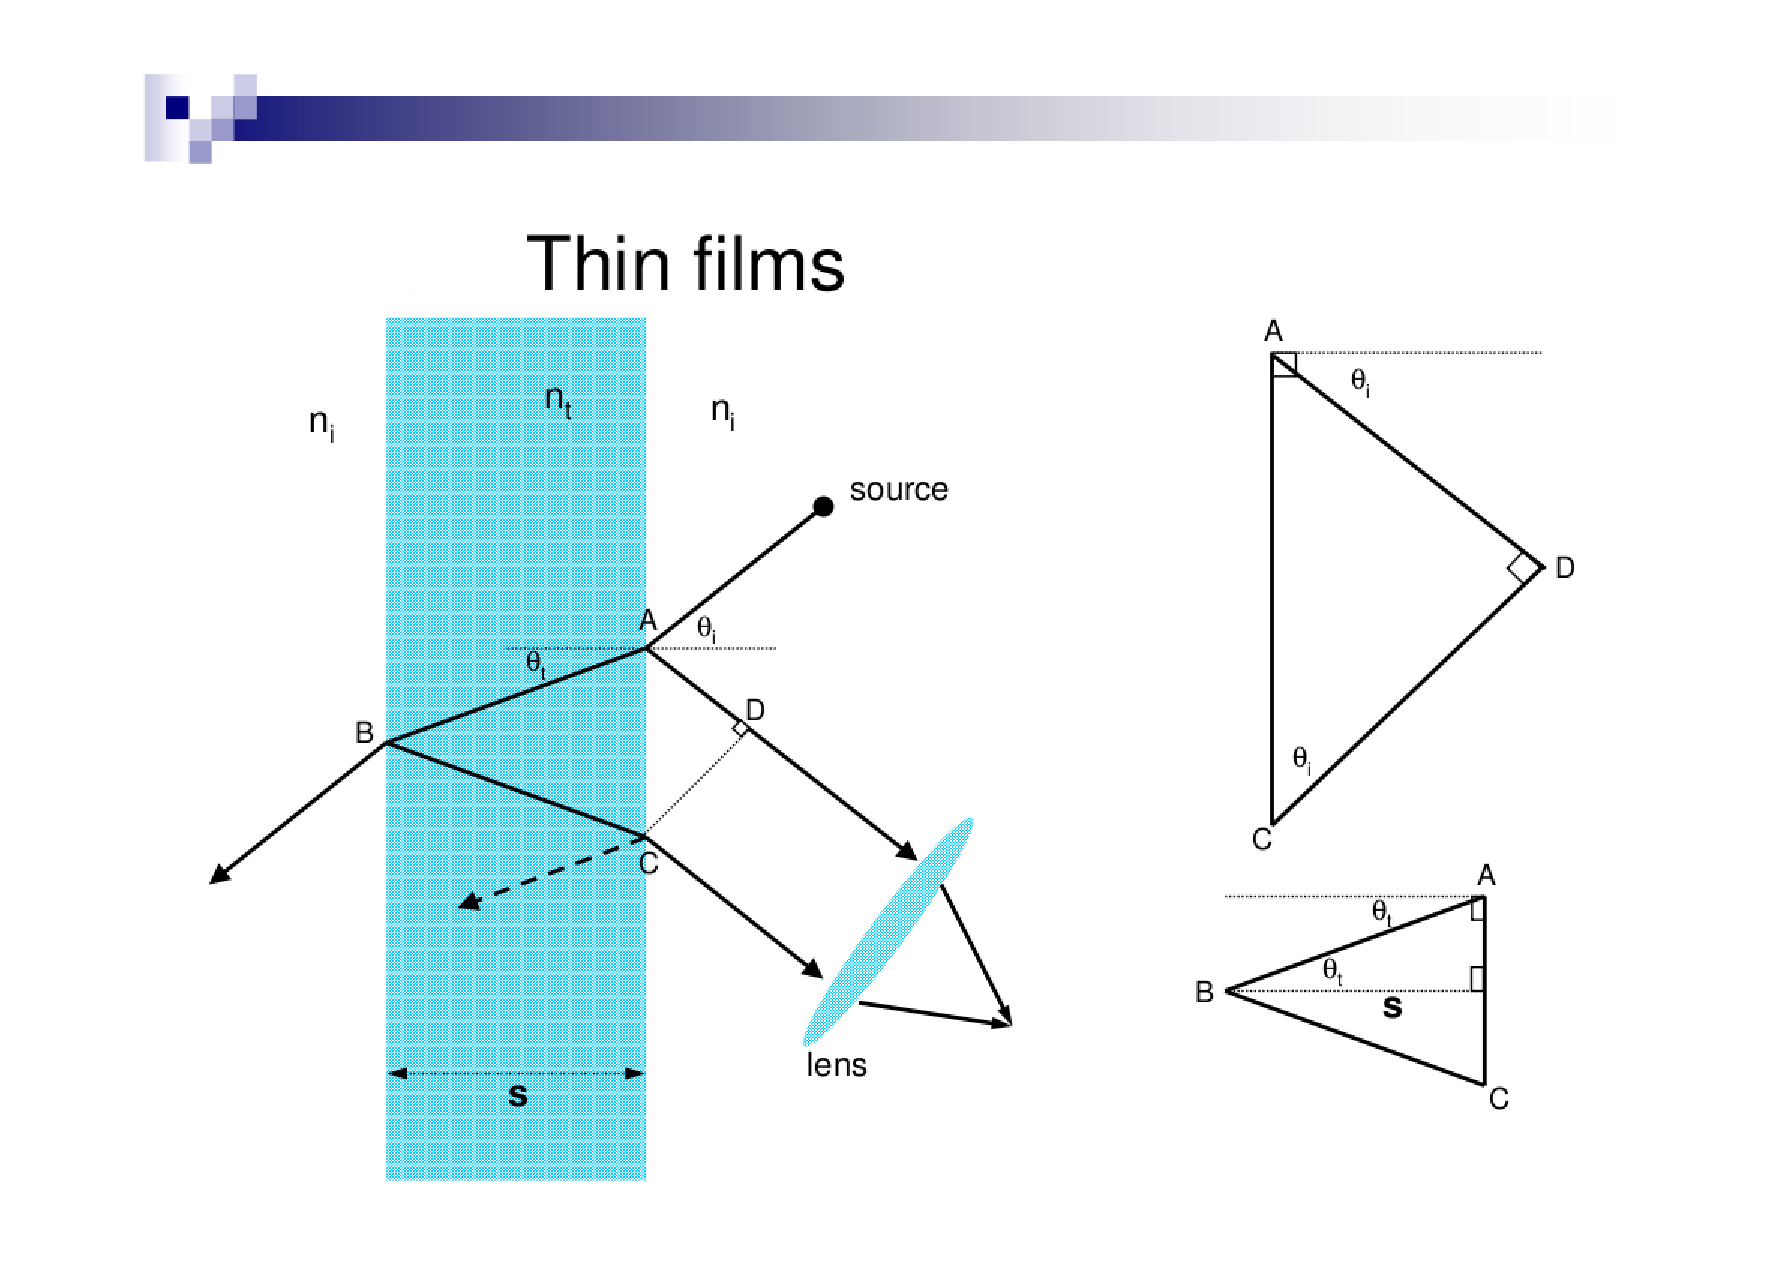
\includegraphics[scale=0.5]{t.eps}
\end{figure}

Optical pld:
\begin{equation*}
d = (AB + BC)n_t - ADn_i
\end{equation*}
but
\begin{itemize}
\item[(i)] \begin{equation*}
AB = BC = \frac{s}{\cos{\theta_t}}
\end{equation*}
\item[(ii)] \begin{equation*}
AD = AC\sin{\theta_i} = AC \frac{n_t}{n_i}\sin{\theta_t}
\end{equation*}
\item[(iii)] \begin{equation*}
\tan{\theta_t} = \frac{AC}{2s}
\end{equation*}
\end{itemize}
combine $(ii)$ and $(iii)$:
\begin{equation*}
AD = 2s \frac{\sin^2{\theta_t}}{\cos{\theta_t}}\frac{n_t}{n_i}
\end{equation*}
\begin{equation*}
d = \frac{2n_t s}{\cos{\theta_t}} - 2sn_i\frac{\sin^2{\theta_t}}{\cos{\theta_t}}\frac{n_t}{n_i} = \frac{2n_t s}{\cos{\theta_t}} \left(1 - \sin^2{\theta_t} \right) = 2n_t s\cos{\theta_t}
\end{equation*}

Phase difference:
\begin{equation*}
\delta = \frac{2 \pi d}{\lambda} - \pi
\end{equation*}
$-\pi$ due to difference in phase between low $n \rightarrow$ high $n$ reflection component to high $n \rightarrow$ low $n$ reflection.
\begin{equation}\boxed{
\delta = \frac{n \pi}{\lambda} n_t s \cos{\theta_t} - \pi
}\end{equation}

If
\begin{equation*}
\delta = 2m\pi
\end{equation*}
-- constructive interference.

If
\begin{equation*}
\delta = (2m+1)\pi
\end{equation*}
-- distructive interference.

Thin films of constant thickness often used to make
\begin{itemize}
\item dichromic mirrors;
\item anti-reflection continges.
\end{itemize}

In practice multiple layers used.

Thin films also formed in nature:
\begin{itemize}
\item oil on water;
\item soap bubble;
\item tapetium lucidium.
\end{itemize}

\subsubsection{Multibeam interference}
Now if a thin parallel layer is coated so that each interface is highly reflective.

\begin{figure}[p!]
\centering
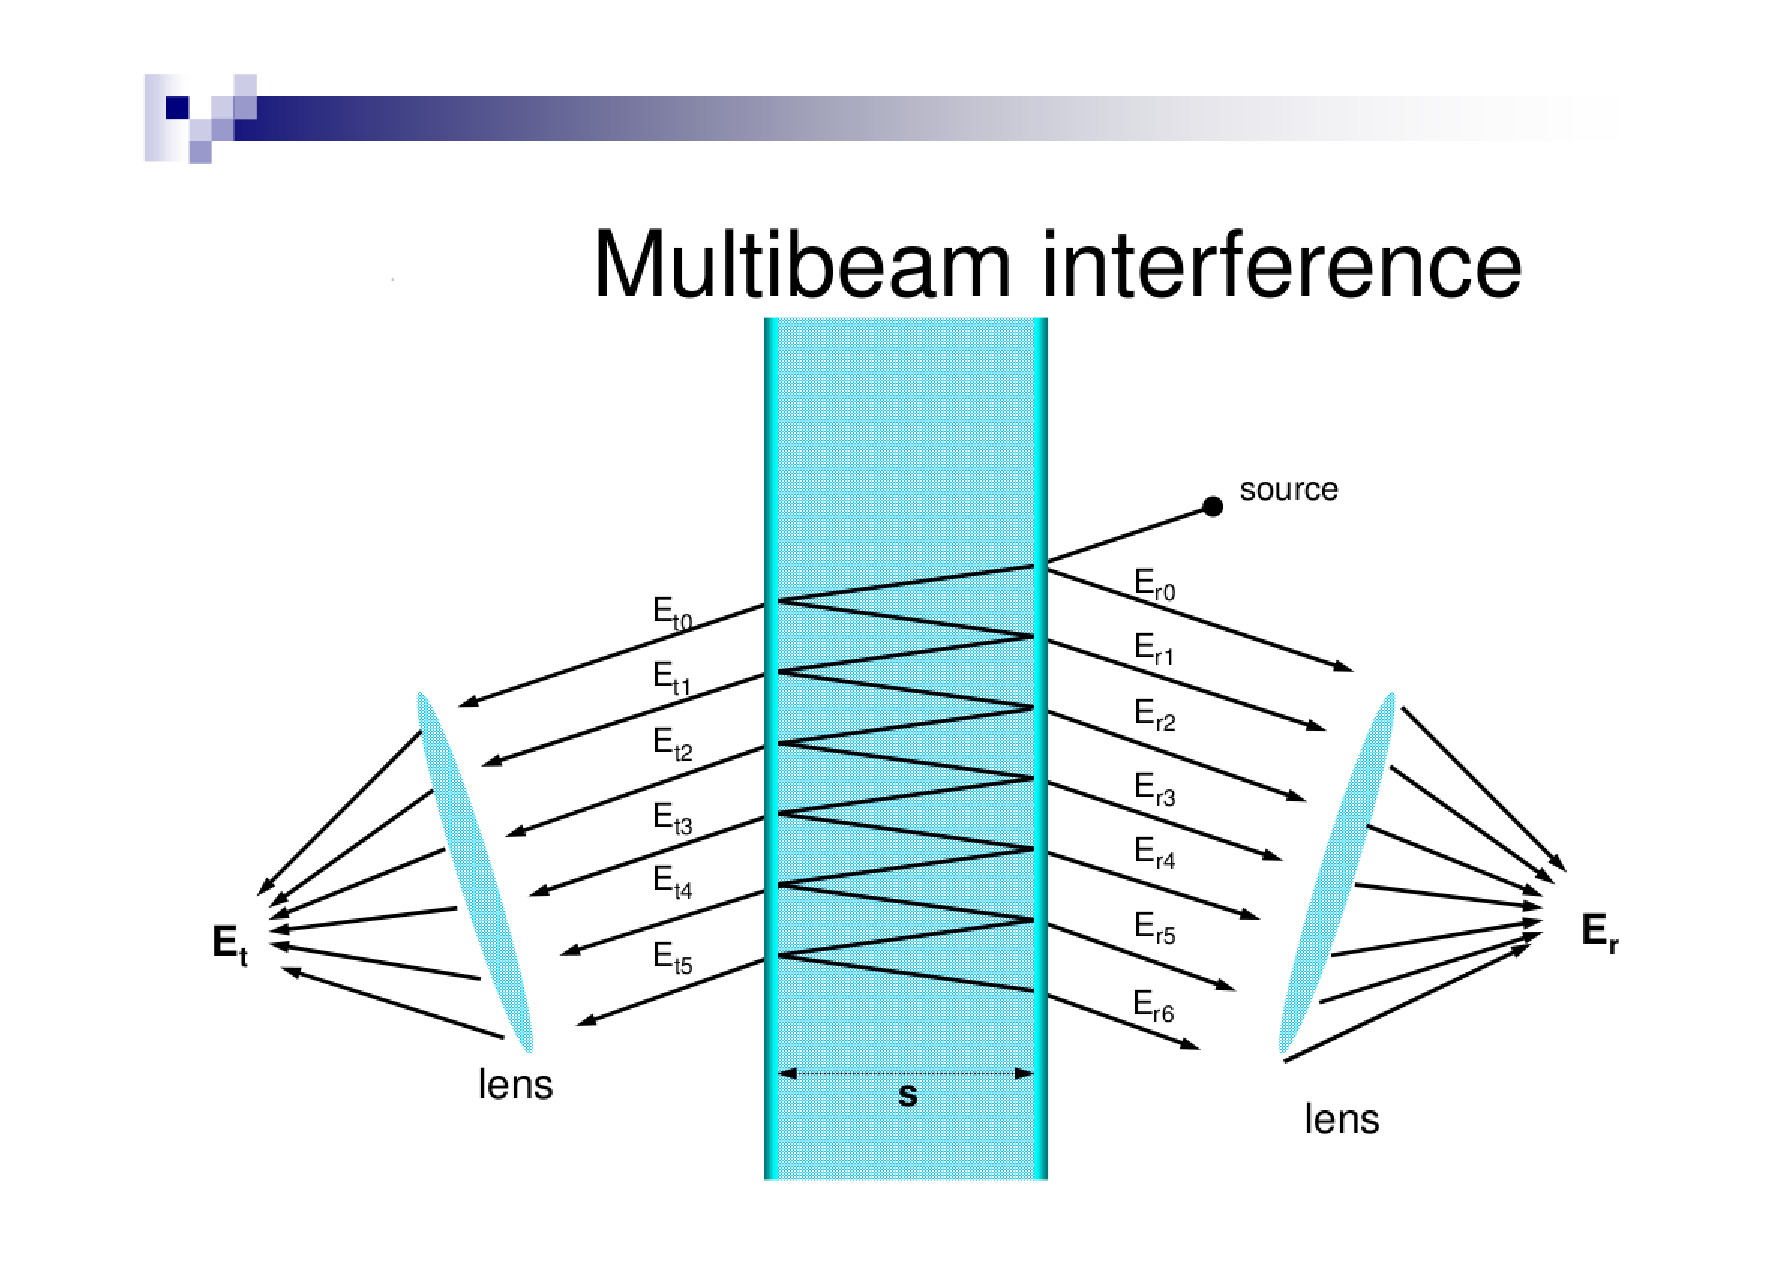
\includegraphics[scale=0.5]{stokes.eps}
\end{figure}
\begin{figure}[p!]
\centering
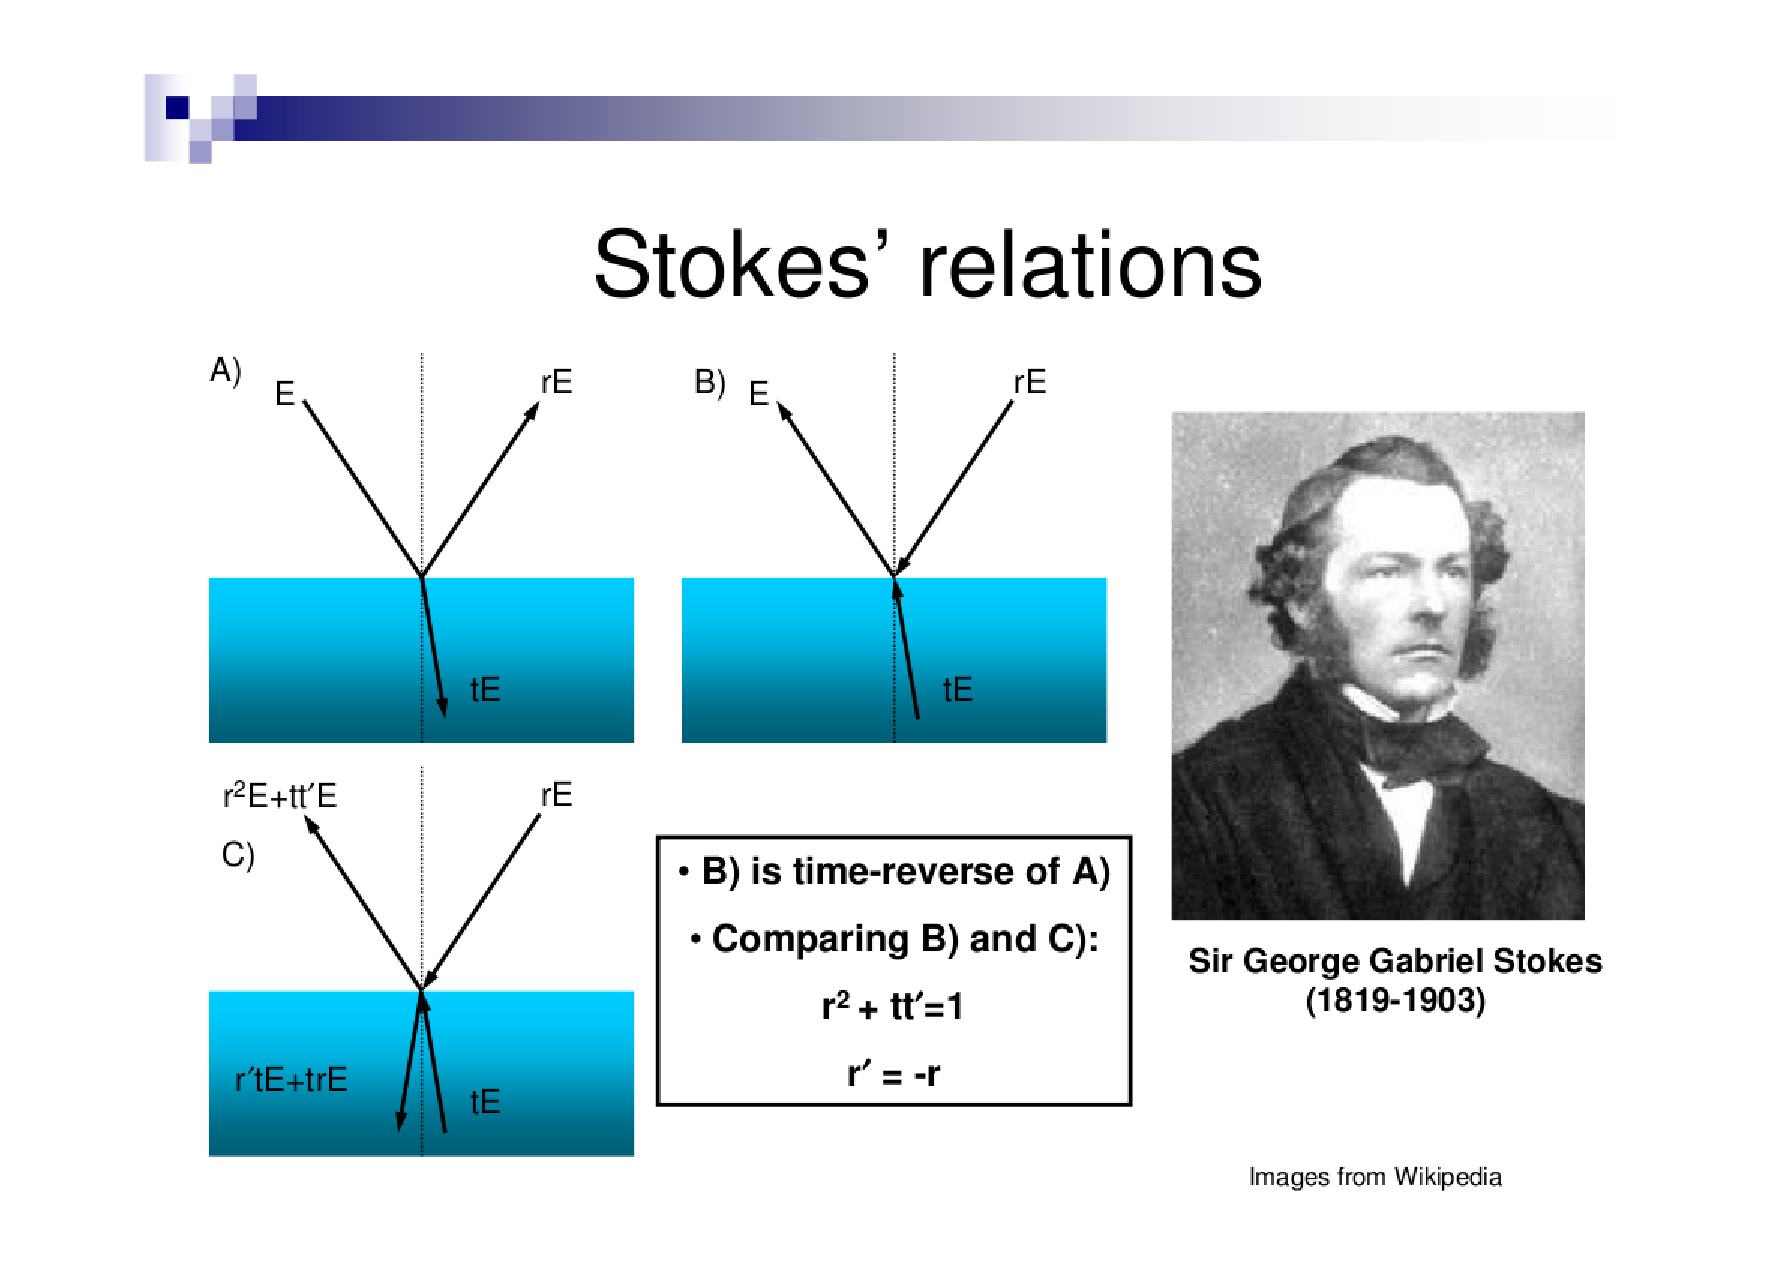
\includegraphics[scale=0.5]{stokes1.eps}
\end{figure}

Stokes' relations are needed.

Consider reflected rays
\begin{equation*}
E_{r_o} = E_o r
\end{equation*}
\begin{equation*}
E_{r_i} = E_o tt' r' e^{ikd}
\end{equation*}
where
\begin{equation*}
d = 2ns\cos{\theta_t}
\end{equation*}
both reflections are internal, so did not need to bother about $\pi$ term.
\begin{eqnarray*}
E_{r_2} = E_o tt' r'^3 e^{i2kd}\\
\vdots \\
E_{r_n} = E_o tt' r'^{(2n-1)} e^{inkd}
\end{eqnarray*}

Total reflected field:
\begin{equation*}
E_r = E_o r + E tt'r'e^{ikd}\left[1 + r^2 e^{ikd} + (r^2e^{i2kd})^2 + ... \right]
\end{equation*}
and this is geometric series.

From Stokes' relations:
\begin{equation*}
r^2 + tt' = 1
\end{equation*}
\begin{equation*}
r' = -r
\end{equation*}
\begin{equation*}
E_r = E_o \left[ r + \frac{tt'r'e^{ikd}}{1 - r^2 e^{ikd}} \right]
\end{equation*}
using Stokes' relations again:
\begin{equation*}
E_r = E_o r \left[\frac{1 - e^{ikd}(r^2 + tt')}{1 - r^2 e^{ikd}} \right]
\end{equation*}
\begin{equation*}
E_r = E_o r \frac{1 - e^{ikd}}{1 - re^{ikd}}
\end{equation*}
\begin{equation*}
\frac{I_r}{I_o} = r^2 \left(\frac{1 - e^{ikd}}{1 - r^2e^{ikd}}\right) \left(\frac{1 - e^{-ikd}}{1 - re^{-ikd}} \right) = 2r^2 \frac{1 - \cos{kd}}{1 - 2r\cos{kd} + r^4}
\end{equation*}

Now reflectance
\begin{equation*}
R = r^2 = 1-T
\end{equation*}

Transmittance
\begin{equation*}
T = tt'
\end{equation*}

So the first Stokes' relation is just a conservation of energy.

Rewrite:
\begin{equation*}
\frac{I_r}{I_o} = \frac{4R\sin^2{(\frac{kd}{2}})}{(1 + R)^2 - 2R(1 - 2 \sin^2{(\frac{kd}{2}}))} = \frac{4R\sin^2{(\frac{kd}{2}})}{(1 + R)^2 + 4R\sin^2{(\frac{kd}{2}})}
\end{equation*}

Define the \textit{coefficient of finesse}:
\begin{equation}\boxed{
F = \frac{4R}{1 - R^2}
}\end{equation}
\begin{equation*}
\frac{I_r}{I_o} = \frac{F\sin^2{(\frac{kd}{2}})}{1 + F\sin^2{(\frac{kd}{2}})}
\end{equation*}

Similarily
\begin{equation}\boxed{
\frac{I_t}{I_o} = \frac{1}{1 + F\sin^2{(\frac{kd}{2}})}
}\end{equation}
this equation is known as \textit{Airy function}.
\begin{figure}[h]
\centering
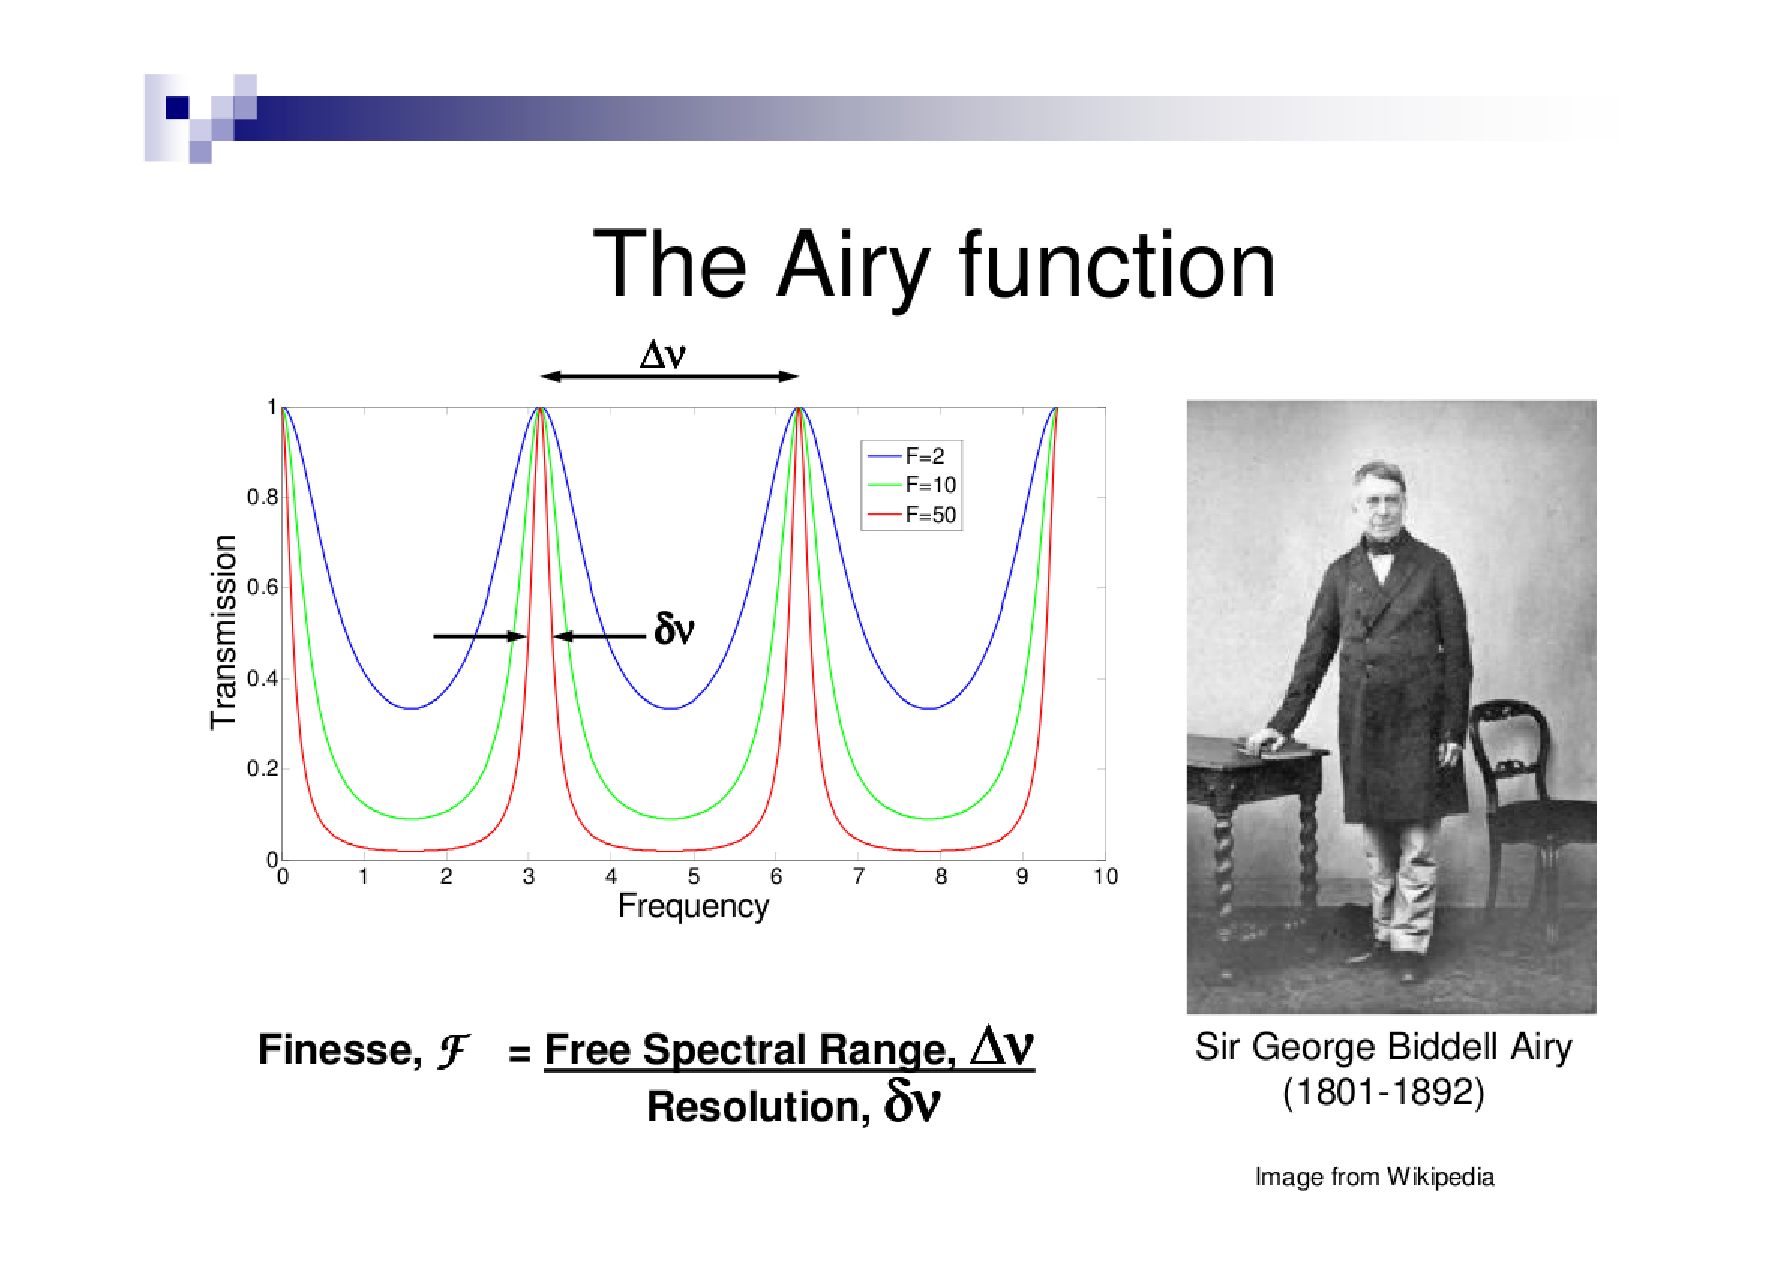
\includegraphics[scale=0.5]{a.eps}
\end{figure}
\begin{enumerate}
\item Free space range $\Delta \nu$
\begin{itemize}
\item Frequency difference between adjacent maxima.
\item Maximum when
\begin{equation*}
\frac{kd}{2} = m\pi
\end{equation*}
\begin{equation*}
m\pi = \frac{2\pi n \nu_m}{c}s \cos{\theta}
\end{equation*}
\begin{equation*}
\nu_m = \frac{mc}{2ns\cos{\theta}}
\end{equation*}
\begin{equation*}
\nu_{m+1} = \frac{(m+1)c}{2ns\cos{\theta}}
\end{equation*}
\begin{equation}\boxed{
\Delta \nu = \nu_{m+1} - \nu_m = \frac{c}{2ns \cos{\theta}}
}\end{equation}
\end{itemize}
\item Peak width \\
Half maximum:
\begin{equation*}
\frac{1}{1 + F\sin^2{(\frac{kd}{2}})} = \frac{1}{2}
\end{equation*}
\begin{equation*}
\sin{\left(\frac{kd}{2}\right)} = \frac{1}{\sqrt{F}}
\end{equation*}
But $F$ is large $\Rightarrow$
\begin{equation*}
\delta (kd) \approx \frac{2}{\sqrt{F}}
\end{equation*}
since angles are small, $\sin{\theta} \approx \theta$. \\
For FWHM:
\begin{equation*}
\delta (kd)_{FWHM} = \frac{4}{\sqrt{F}}
\end{equation*}
\begin{equation*}
n\frac{4\pi s}{c}\cos{\theta}\delta \nu = \frac{4}{\sqrt{F}}
\end{equation*}
\begin{equation}\boxed{
\delta \nu = \frac{c}{\sqrt{F}n\pi s \cos{\theta}}
}\end{equation}
\end{enumerate}

Finesse, $\mathcal{F}$:
\begin{equation*}
\mathcal{F} = \frac{\Delta \nu}{\delta \nu} = \frac{\pi \sqrt{F}}{2}
\end{equation*}
for a mirror:
\begin{equation}\boxed{
\mathcal{F} = \frac{\pi \sqrt{R}}{1 - R}
}\end{equation}

\subsubsection{The Fabri-Perot etalons}
\begin{figure}[h!]
\centering
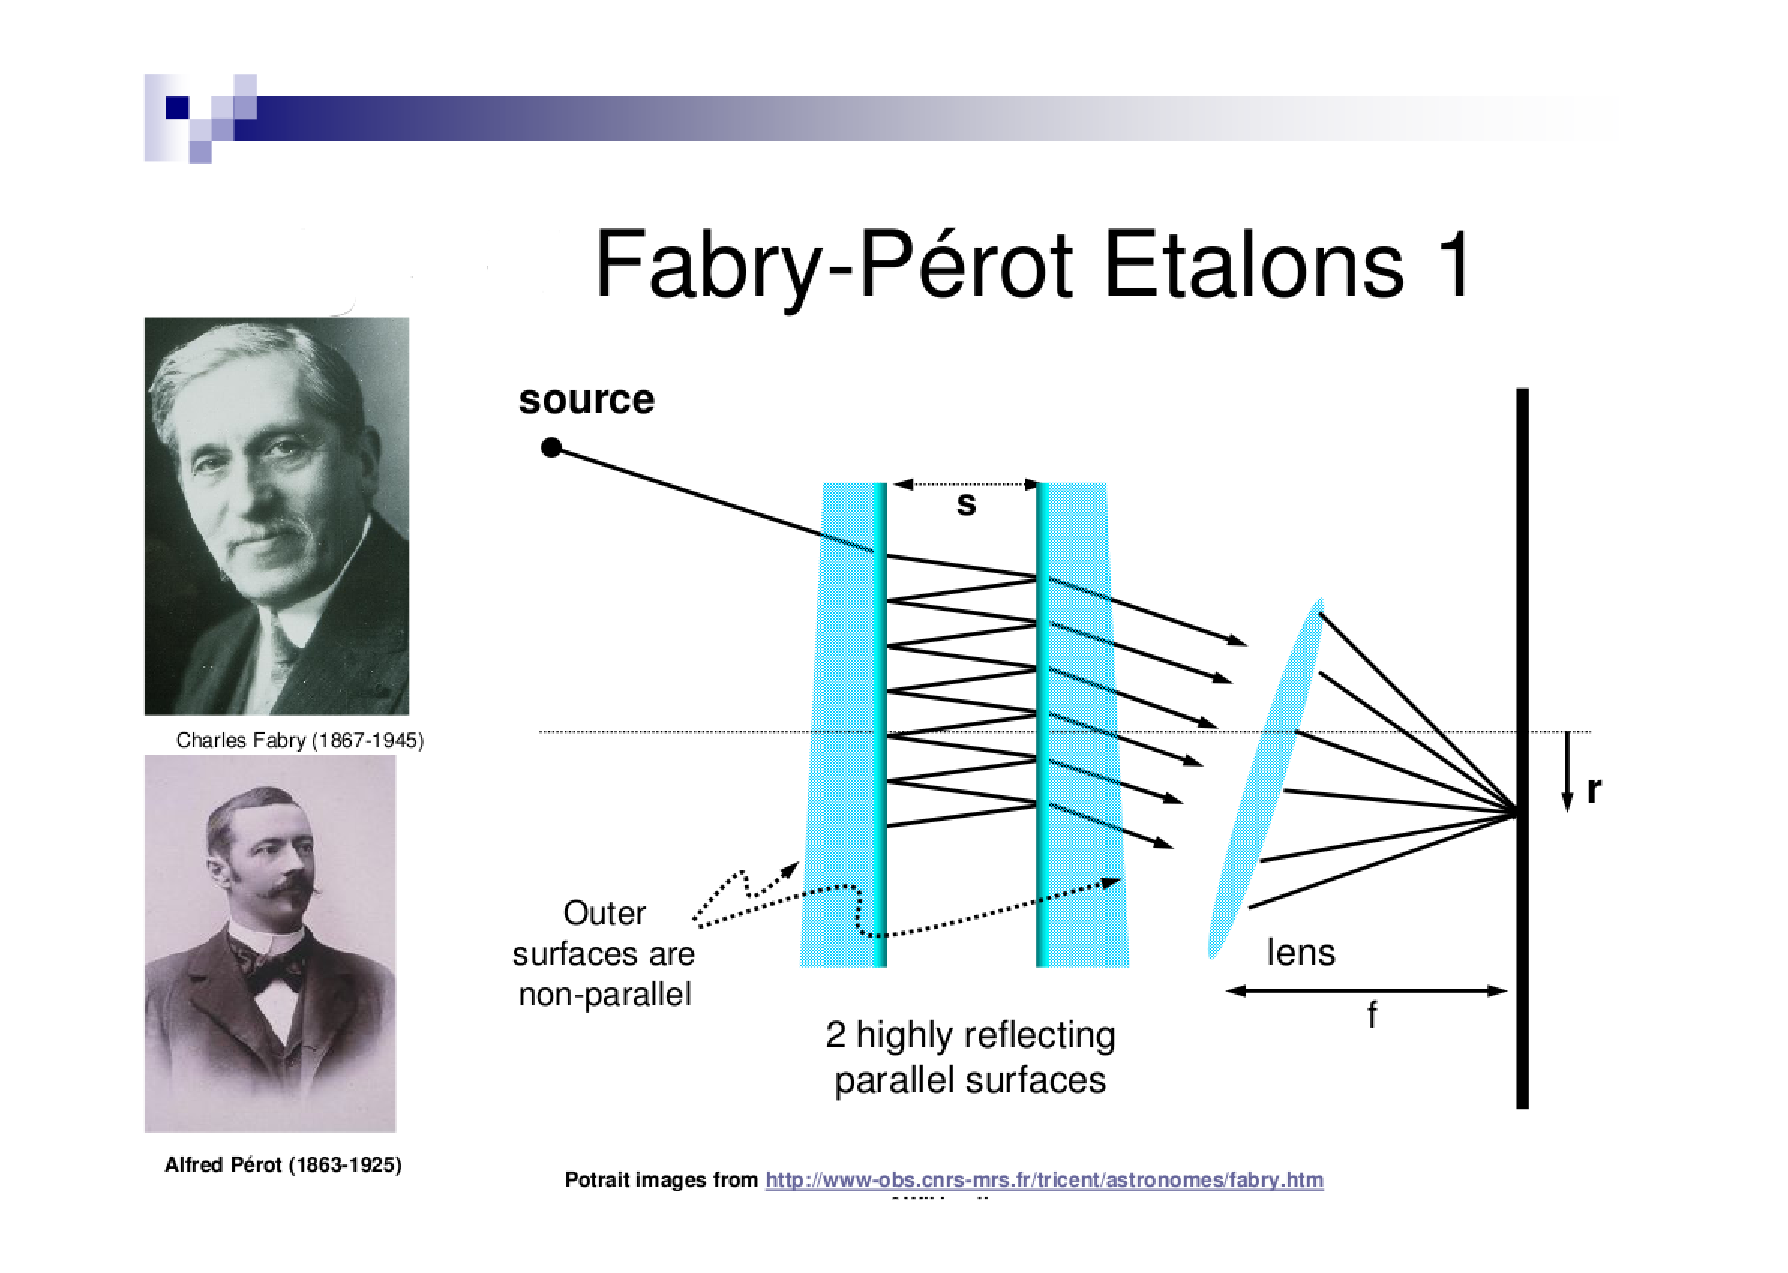
\includegraphics[scale=0.5]{a1.eps}
\end{figure}
\begin{equation*}
n = 1
\end{equation*}

Bright fringe occures when
\begin{equation*}
m\pi = \frac{2d}{\lambda} = \frac{2\pi s \cos{\theta_m}}{\lambda}
\end{equation*}
a changing source results in a range of $\theta$.

For small $\theta$:
\begin{equation*}
m = \frac{2s}{\lambda}\left(1 - \frac{\theta_m ^2}{2} \right)
\end{equation*}
for $\theta = 0$
\begin{equation*}
m_0 = \frac{2s}{\lambda}
\end{equation*}

Let
\begin{equation*}
p = m_0 - m
\end{equation*}
therefore
\begin{equation*}
m_0 - p = m_0 - \frac{s\theta_p ^2}{\lambda}
\end{equation*}
\begin{equation*}
\theta_p = \sqrt{\frac{p \lambda}{s}}
\end{equation*}
\begin{figure}[h!]
\centering
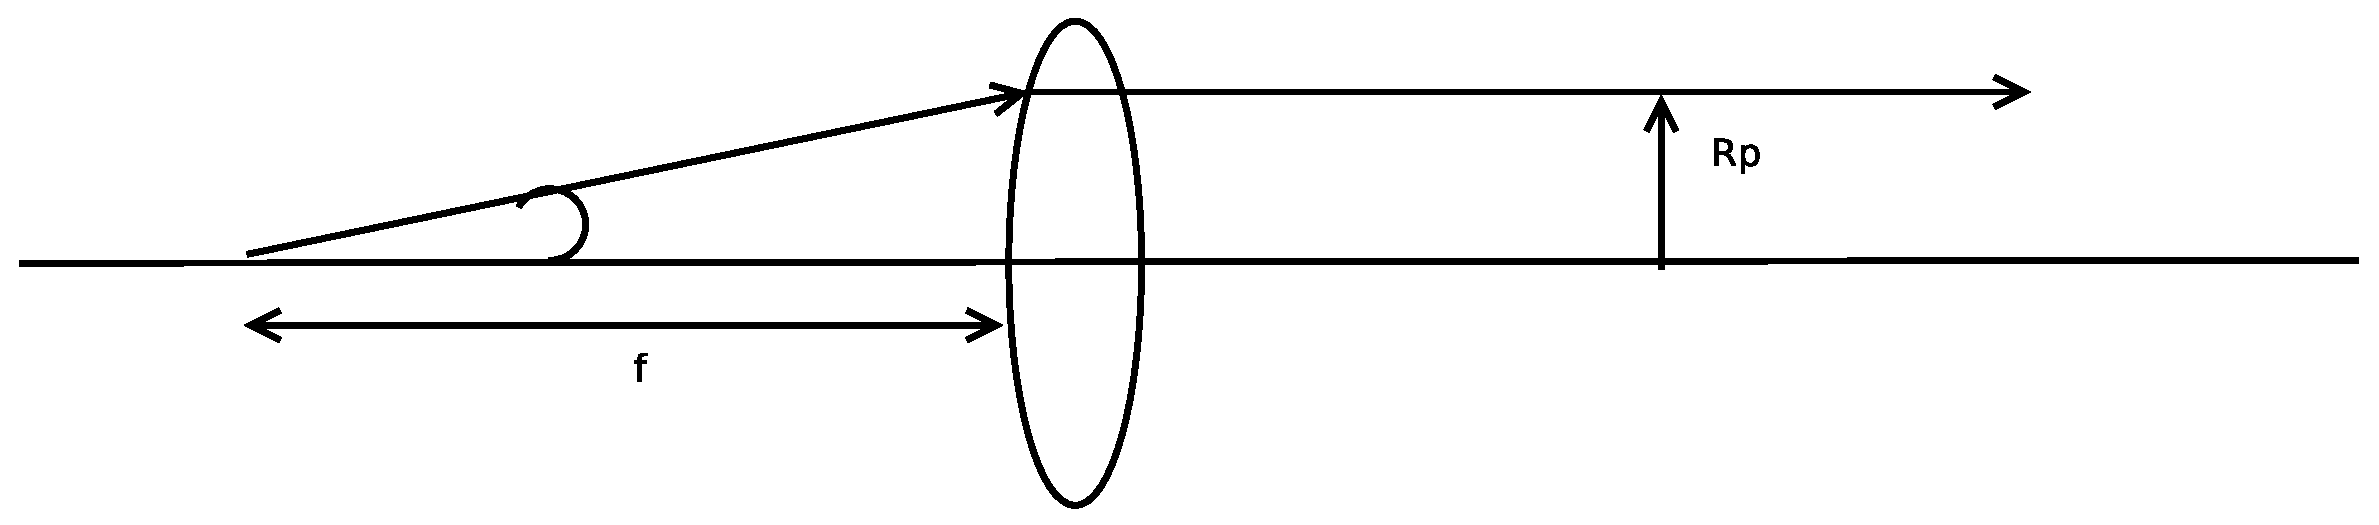
\includegraphics[scale=0.25]{a2.eps}
\end{figure}
\begin{equation*}
R_p = f\theta_p = f\sqrt{\frac{p\lambda}{s}}
\end{equation*}

\section{Diffraction}
\subsection{The Huygens-Frensel principle}
Combine Huygens wavelets with interference.

Postulated in 1818, 43 years before Maxwell equations. Eventually derrived from wave equation by Kirchoff in 1882.

\subsection{The Huygens-Frensel integral}
\begin{figure}[h!]
\centering
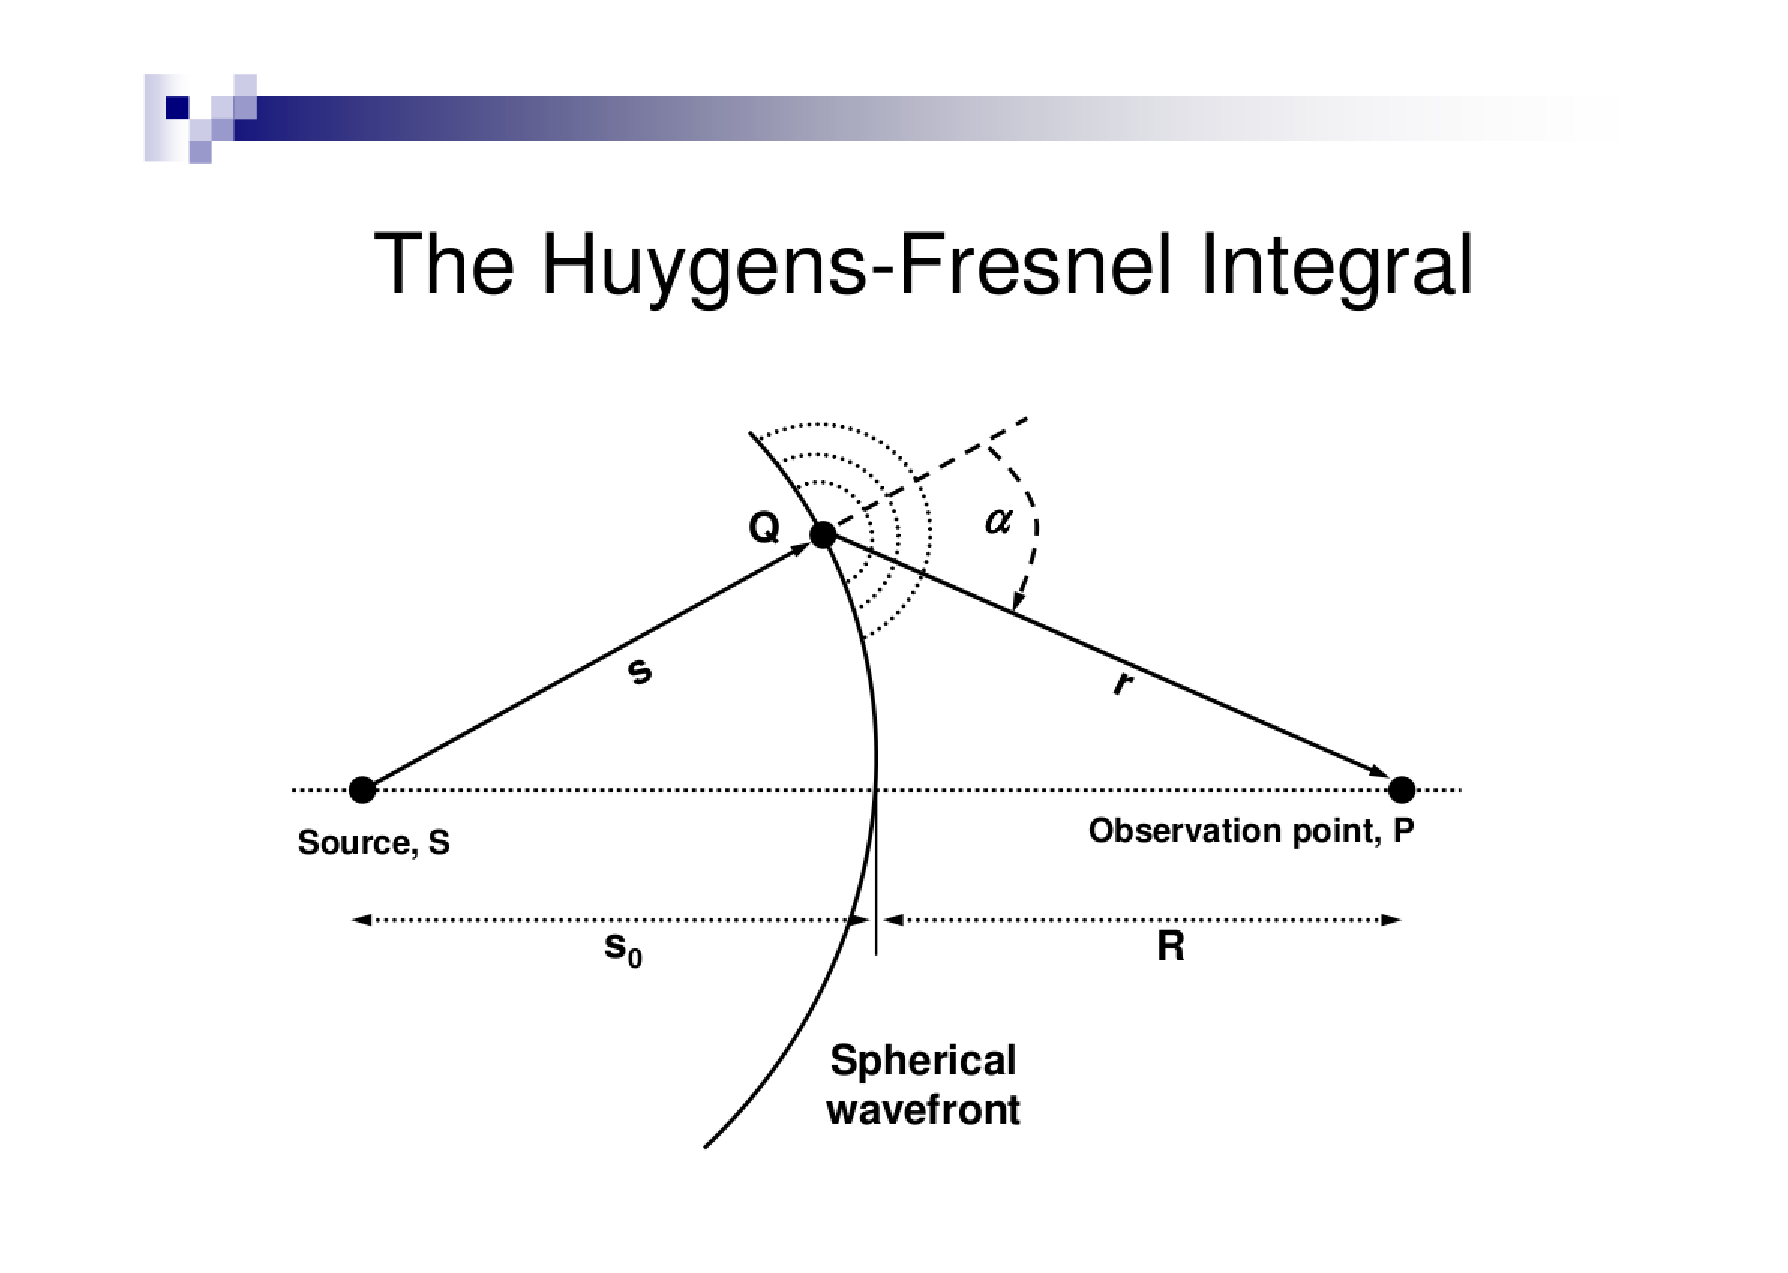
\includegraphics[scale=0.5]{hu.eps}
\end{figure}
Field at $Q$:
\begin{equation*}
E(Q) ~ \frac{e^{iks}}{s}
\end{equation*}

In genereal, field radiated from $Q$ to $P$ depends on angle. It is described by some \textit{obliquity factor} $K(\alpha)$.

Contribution to field at $P$ that at $Q$:
\begin{equation*}
dE = K(\alpha)\epsilon' \frac{e^{iks}}{s}\frac{e^{ikr}}{r}dA
\end{equation*}
$\epsilon'$ -- field strength per unit area.

Total field at $P$:
\begin{equation}\boxed{
E(P) = \epsilon' \frac{e^{iks}}{s} \int \int K(\alpha) \frac{e^{ikr}}{r}dA
}\end{equation}
on the unabstructed area.

And that is the Huygens-Frensel integral.

Note:
\begin{enumerate}
\item HFI does not consider polarisation.
\item Is not always solvable.
\end{enumerate}

\begin{figure}[p!]
\centering
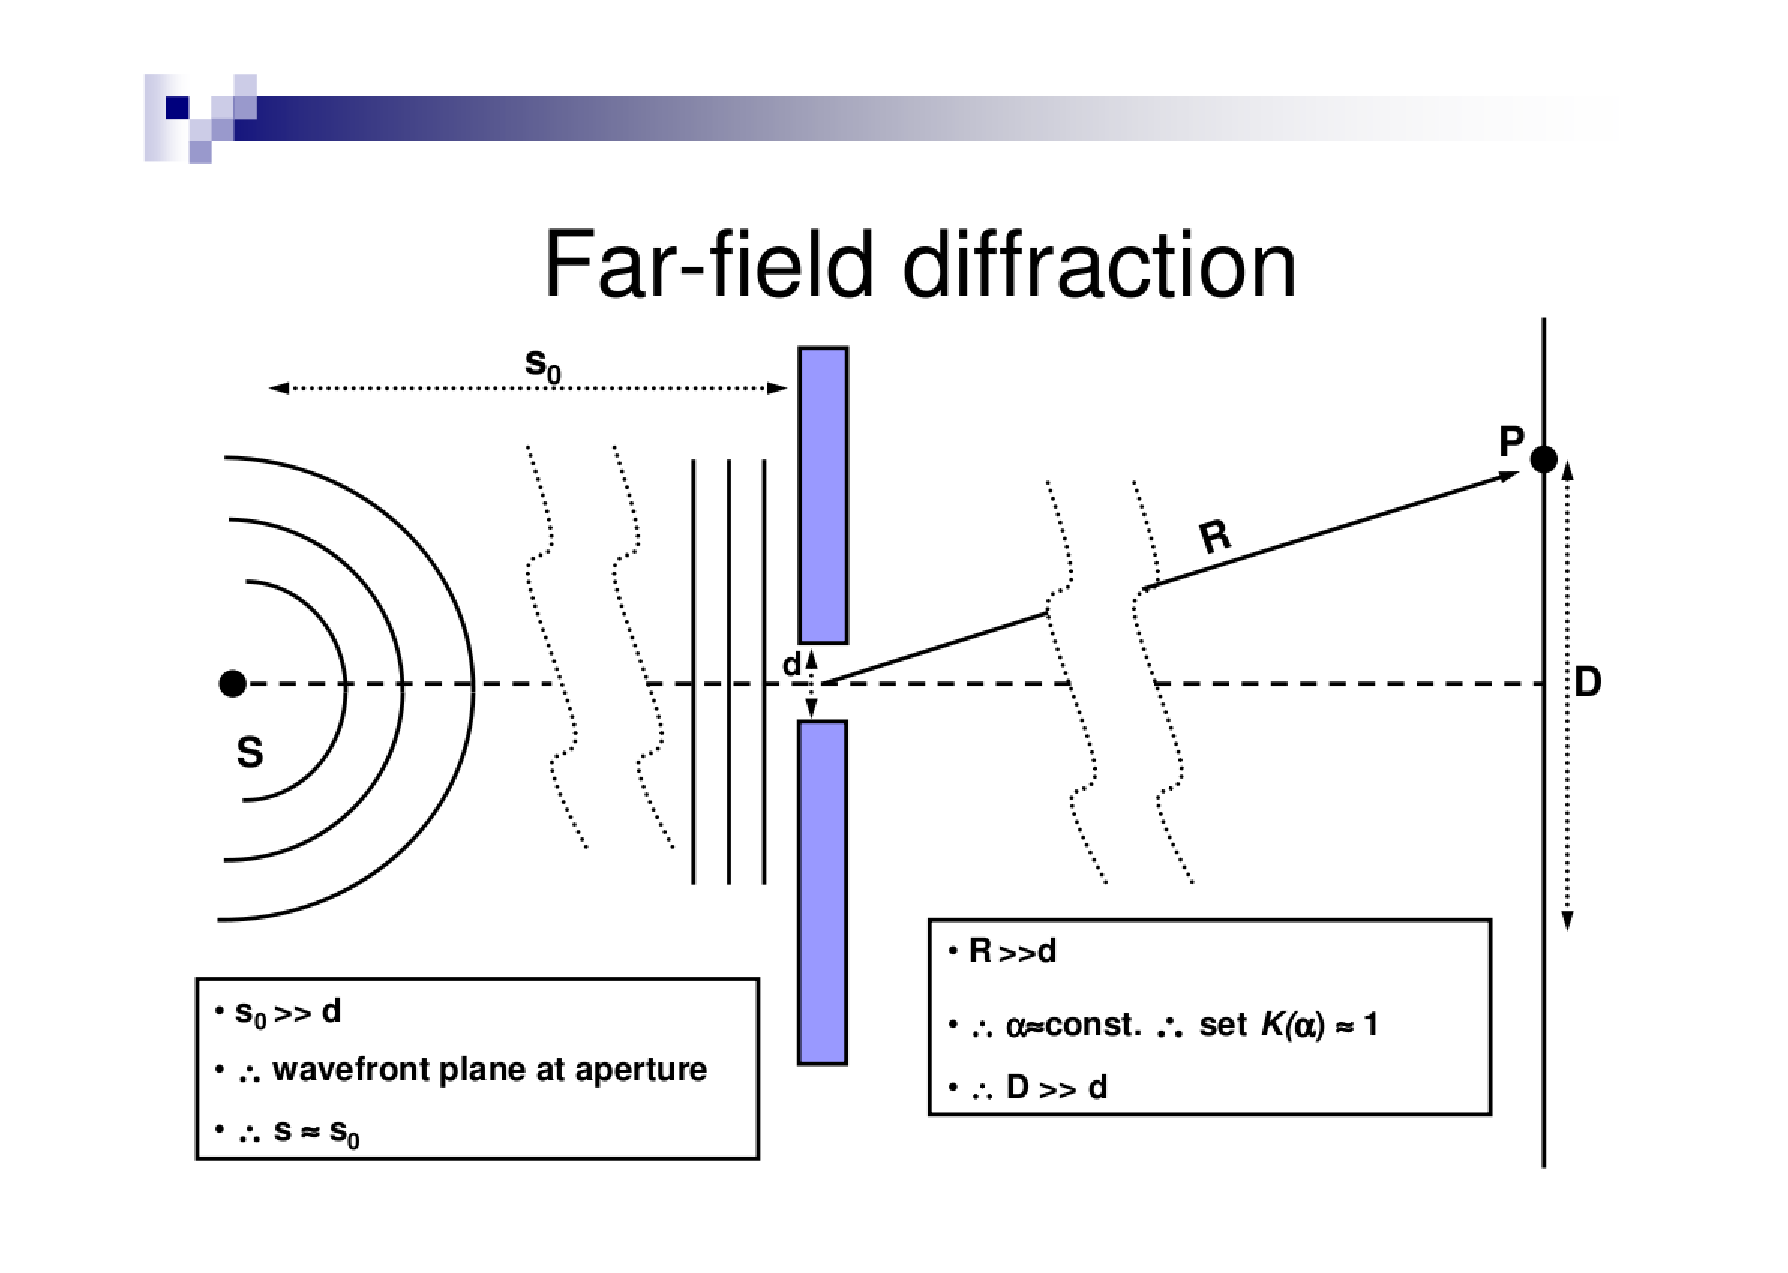
\includegraphics[scale=0.5]{fd.eps}
\end{figure}
\begin{figure}[p!]
\centering
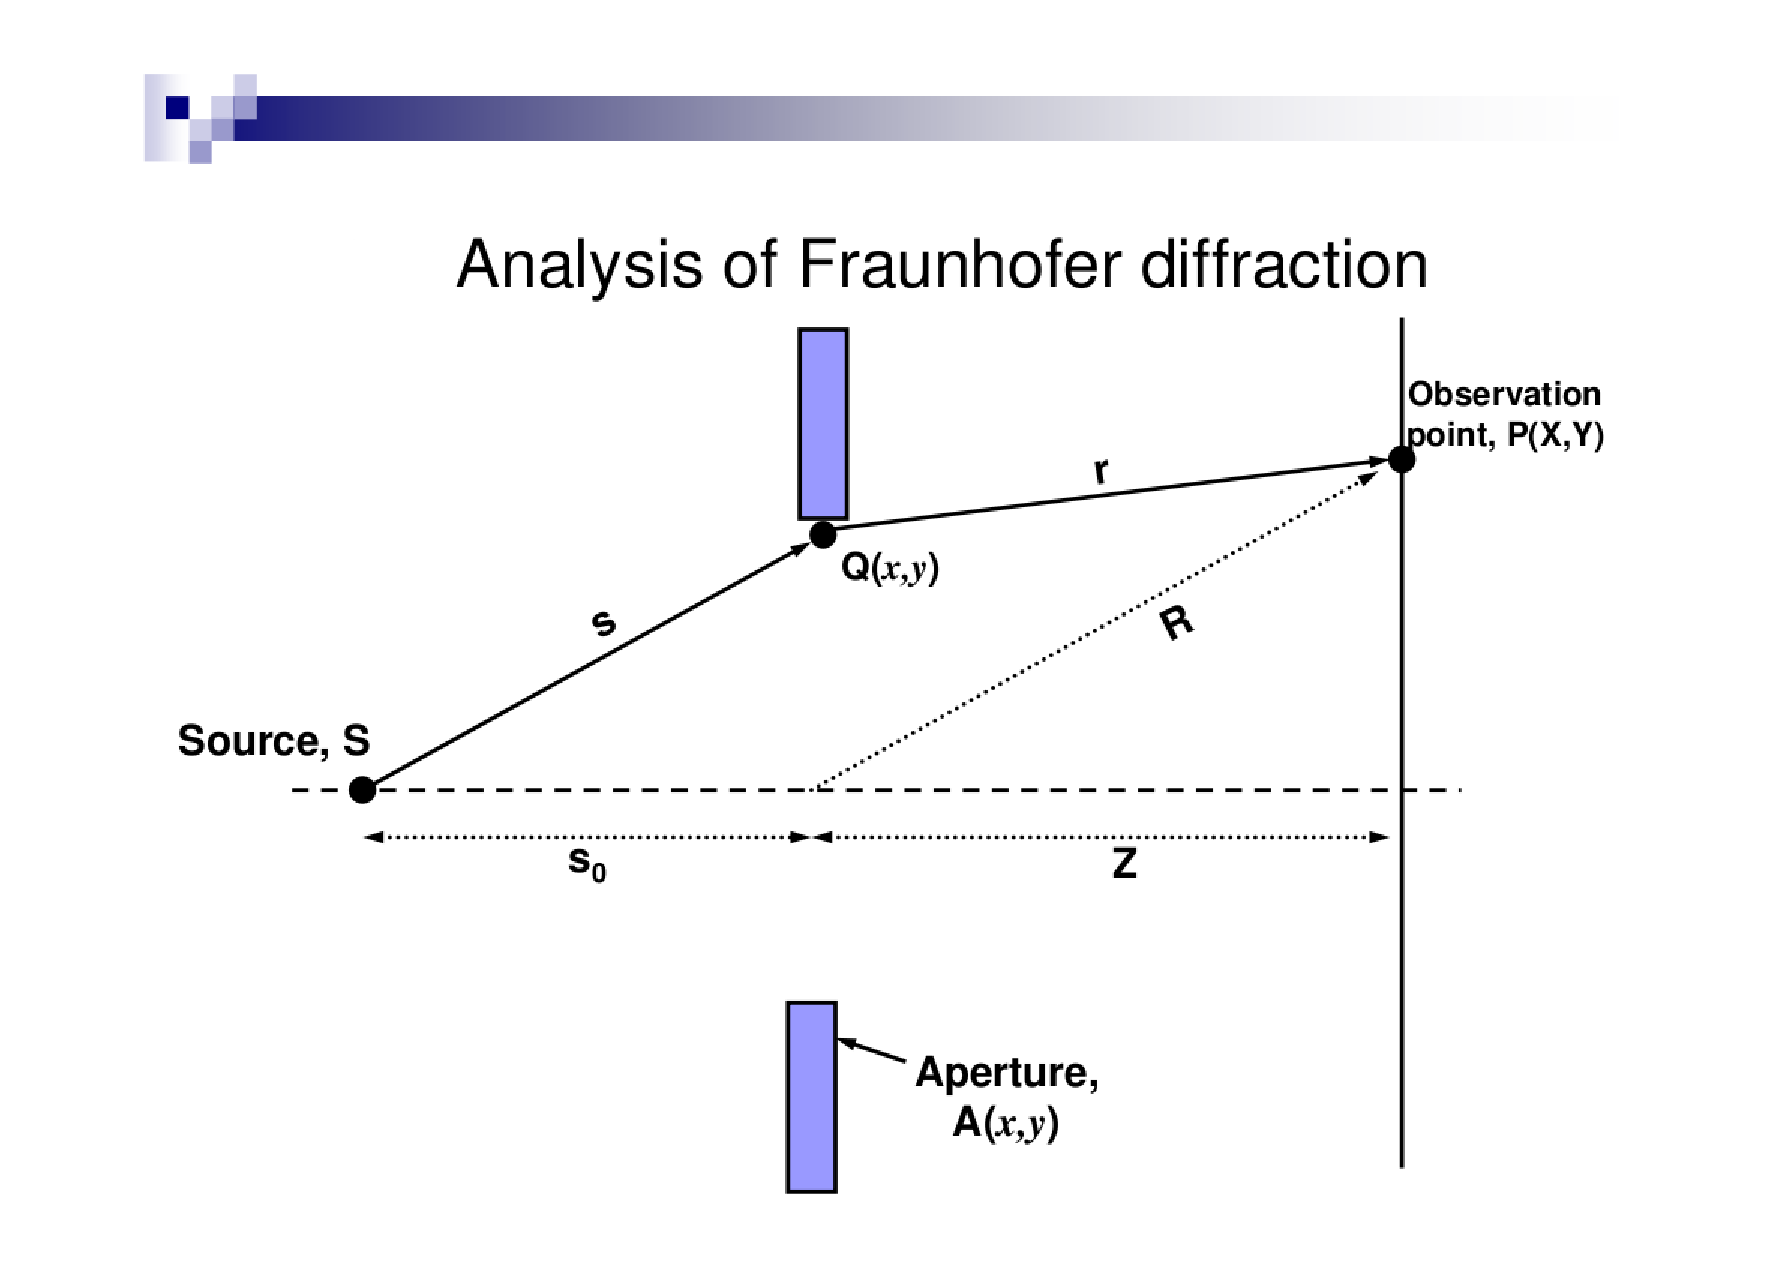
\includegraphics[scale=0.5]{fd1.eps}
\end{figure}

Will now consider two special cases:
\begin{itemize}
\item[(i)] Fraunhofer diffraction;
\item[(ii)] Frensel diffraction.
\end{itemize}

\subsection{Fraunhofer diffraction}
Fraunhofer diffraction is a special case when
\begin{equation*}
r \approx R + \delta r(x,y)
\end{equation*}
where $R >> \delta r, \delta r$ is linear in $x$ and $y$.

These conditoins are satisfied when $SQ = QP >>$ aperture size. This is called far field diffraction.

\begin{itemize}
\item[(i)] Obliquity angle $\alpha \approx const$ therefore $K$ is $const$ (set $1$)
\item[(ii)] $x,y << R$
\item[(iii)] $x,y << X,Y$
\item[(iv)] $s \approx s_0$
\end{itemize}

Pattern becomes large in far field.

HFI becomes:
\begin{equation}\boxed{
E(X,Y) = \frac{\epsilon}{R} \int \int e^{ikr}dA
}\end{equation}
where
\begin{equation*}
\epsilon = \epsilon' \frac{e^{iks}}{s}
\end{equation*}

From Pythagorus:
\begin{flalign*}
r^2 & = (X - x)^2 + (Y - y)^2 + Z^2 \\
& = X^2 + Y^2 + Z^2 - 2(xX + yY) + x^2 +y^2 \\
& = R^2 - 2(xX + yY)\\
\end{flalign*}
\begin{equation*}
r \approx R(1 - \frac{2}{R^2}(xX + yY))^{\frac{1}{2}}
\end{equation*}
since $x,y < R$, apply binominal expansion:
\begin{equation*}
r \approx R \left( 1 - \frac{(xX + yY)}{R^2} + \hdots \right)
\end{equation*}
\begin{equation*}
E(X,Y) = \frac{\epsilon}{R} e^{ikR}\int \int e^{-ik\frac{(xX + yY)}{R}}dx dy
\end{equation*}

Describing aperture with a function $A(x,y)$:
\begin{equation}\boxed{
E(X,Y) = \frac{\epsilon}{R} e^{ikR}\int_{-\infty} ^\infty \int_{-\infty} ^\infty A(x,y) e^{-ik\frac{(xX + yY)}{R}}dx dy
}\end{equation}

If aperture is circularly symmetric, often convinient to use polar coordinates instead of Cartesian.
\begin{equation*}
\begin{gathered}
x = u \cos{\phi}\\
y = u \sin{\phi}\\
X = U \cos{\Phi}\\
Y = U \sin{\Phi}\\
\end{gathered}
\end{equation*}
\begin{equation}\boxed{
E(U) = \frac{\epsilon e^{ikR}}{R} \int_{0} ^\infty \int_{0} ^{2\pi} A(u)e^{-\frac{ikuU}{R}\cos{(\phi - \Phi)}} udud\phi
}\end{equation}

Since aperture and diffraction pattern are circularly symmetric and independent of $\Phi$, we can set $\Phi = 0$. Then
\begin{equation*}
\int_{0} ^{2\pi} e^{-\frac{ikuU}{R}\cos{(\phi)}} d\phi = 2\pi J_0 \left(\frac{kuU}{R} \right)
\end{equation*}

Thus
\begin{equation}\boxed{
E(U) = \frac{\epsilon e^{ikR}}{R} 2\pi \int_{-\infty} ^\infty A(x)e^{\frac{ikxX}{R}}dx
}\end{equation}

\subsubsection{Single slit}
\begin{itemize}
\item variation in only $x-$direction;
\item need to integrate only $1D$.
\end{itemize}
\begin{equation*}
E(X) = \frac{\epsilon e^{ikR}}{R} \int_{-\infty} ^\infty A(x)e^{\frac{ikxX}{R}}dx
\end{equation*}
where $\epsilon$ is now strength per unit length of aperture.

For a single slit:
\begin{equation*}
A(x) = 1
\end{equation*}
for $|x| \leq \frac{a}{2}$
\begin{equation*}
A(x) = 0
\end{equation*}
for $|x| > \frac{a}{2}$
where $a$ is width of the slit.
\begin{flalign*}
E(x) & = \frac{\epsilon e^{ikR}}{R} \int_{-\frac{a}{2}} ^\frac{a}{2} e^{-\frac{ikxX}{R}}dx\\
& = \frac{\epsilon e^{ikR}}{R} \left[ \frac{e^{-\frac{ikxX}{R}}}{e^{-\frac{ikX}{R}}} \right]^\frac{a}{2} _{-\frac{a}{2}}\\
& = \frac{\epsilon e^{ikR}}{R}\frac{e^{-\frac{ikaX}{2R}} - e^{\frac{ikaX}{2R}}}{-\frac{ikX}{R}}\\
& = \frac{\epsilon e^{ikR}}{R} a \frac{2R}{kaX} \sin{\frac{kaX}{2R}}\\
& = a \frac{\epsilon e^{ikR}}{R} sinc{\frac{kaX}{2R}}\\
\end{flalign*}
\begin{equation}\boxed{
I(X) = I(0)sinc^2\frac{kxX}{2R}
}\end{equation}

\subsubsection{A rectangular aperture}
\begin{figure}[h!]
\centering
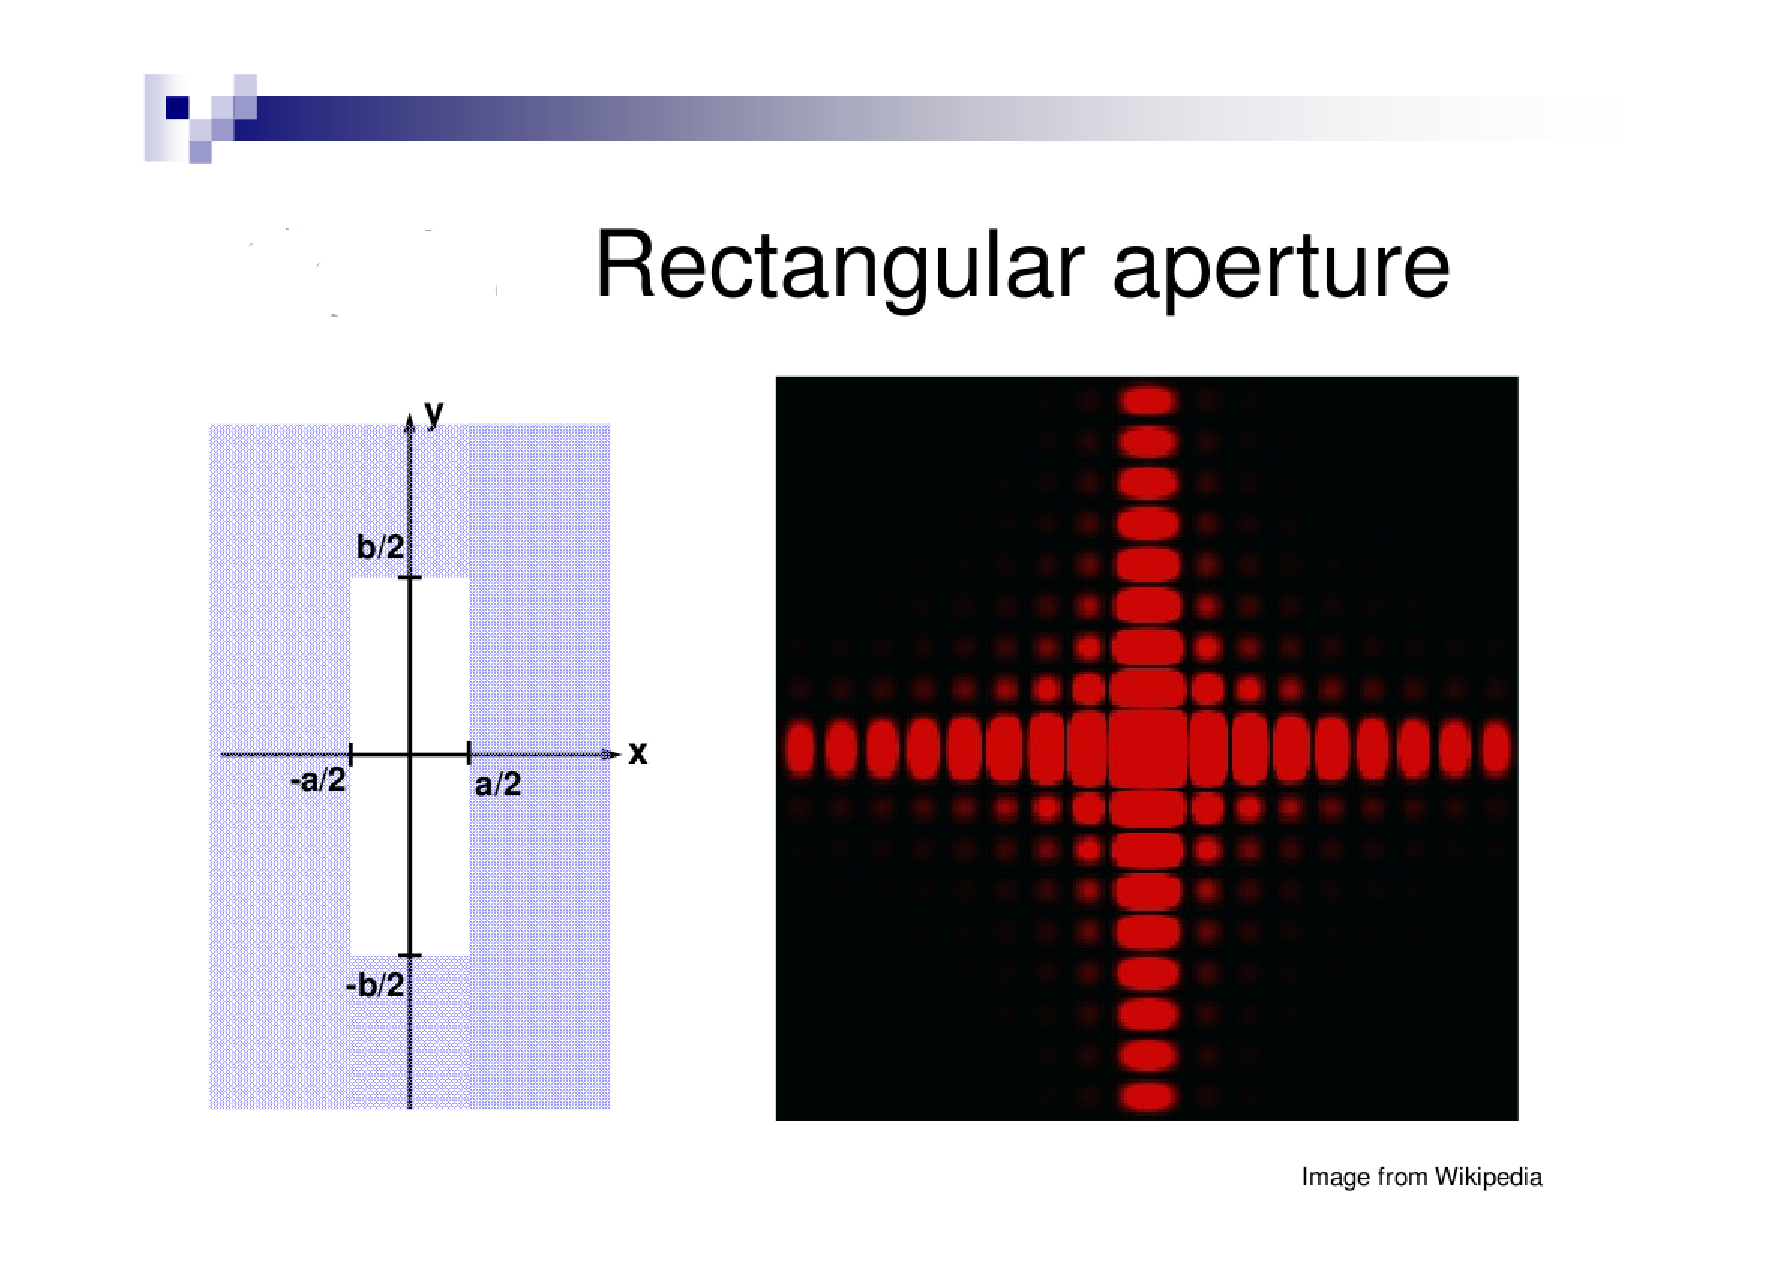
\includegraphics[scale=0.5]{rec.eps}
\end{figure}

\subsubsection{Circular aperture}
\begin{figure}[h!]
\centering
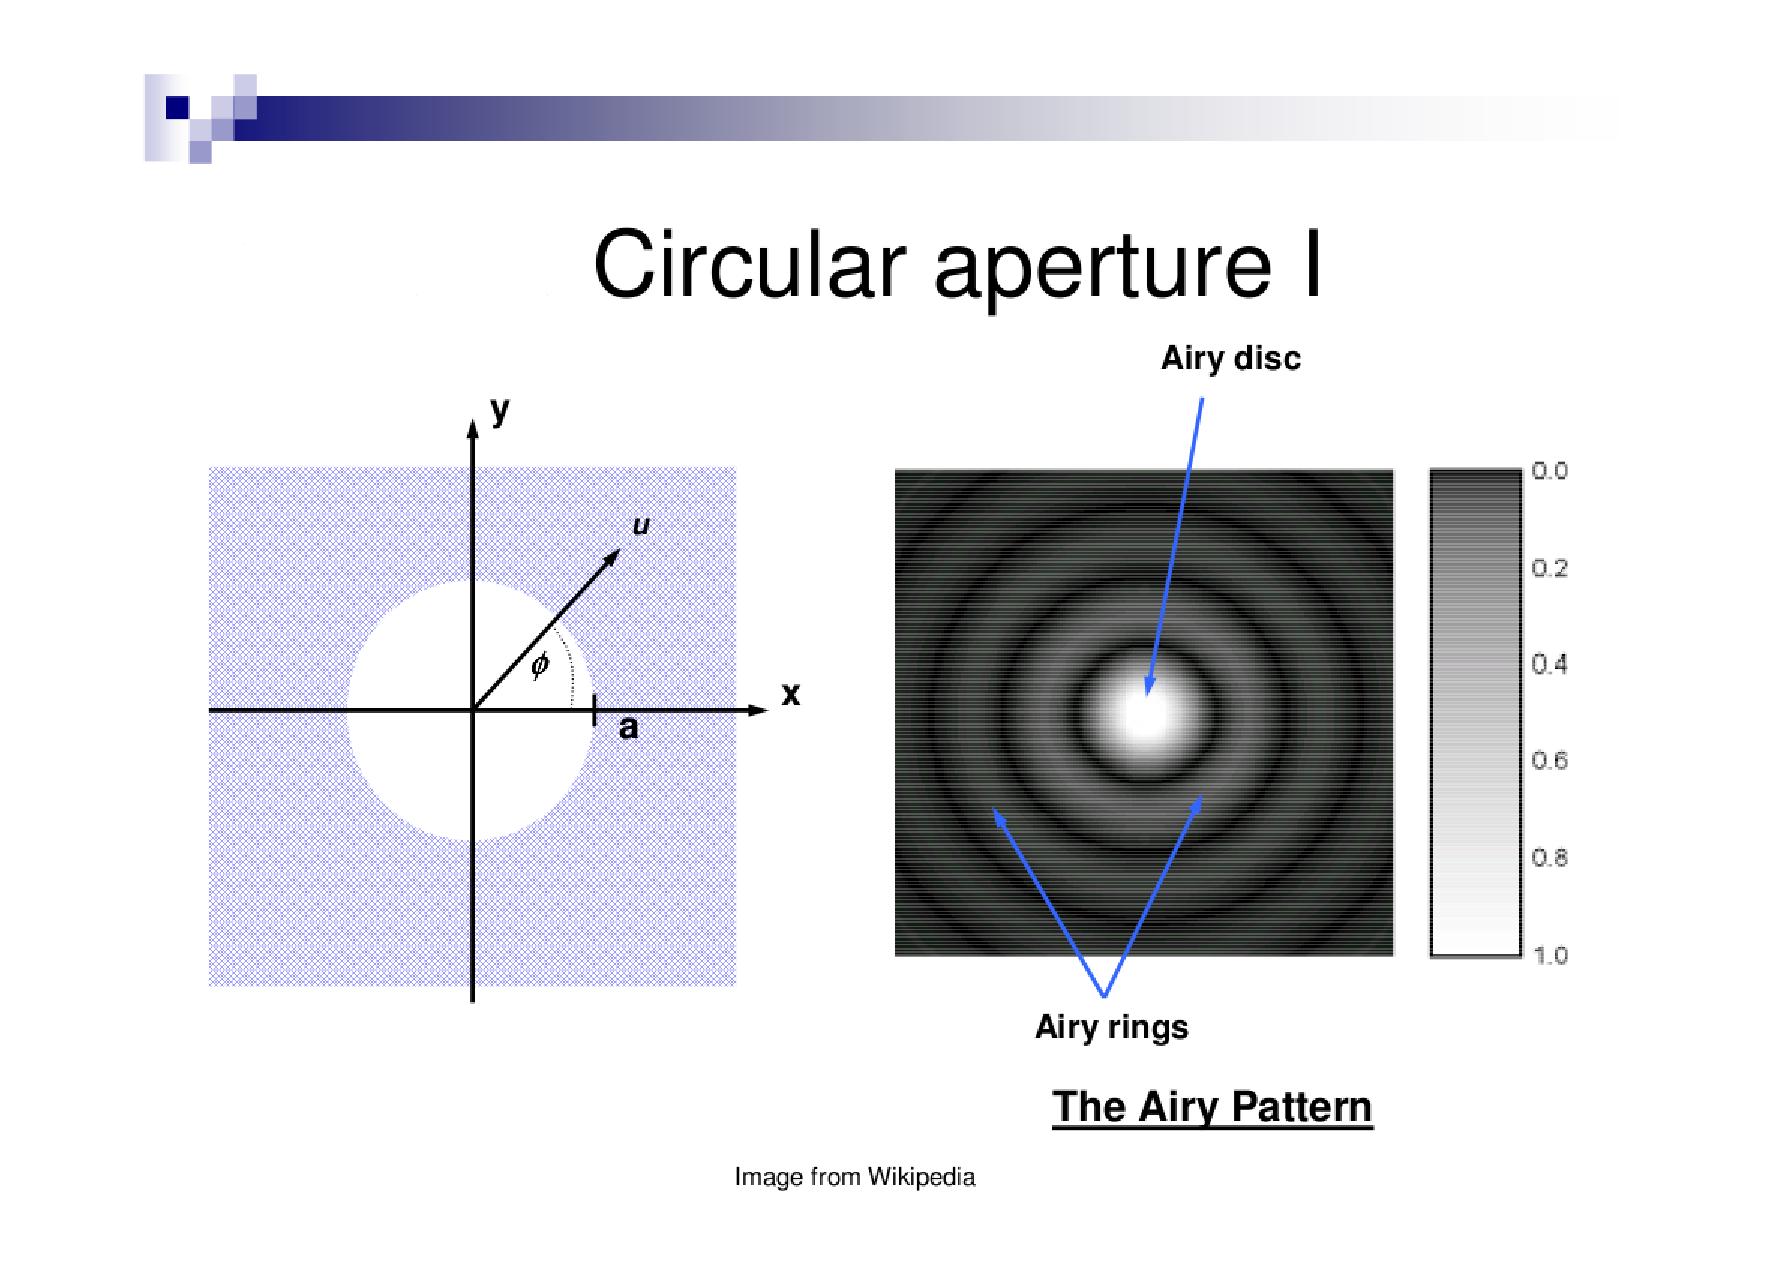
\includegraphics[scale=0.5]{circ.eps}
\end{figure}
For a circular aperture of radius $a$:
\begin{equation*}
\begin{array}{c c}
A(u) = 1 & u\leq a \\
A(u) = 0 & u > a \\
\end{array}
\end{equation*}

Property of Bessel's function is:
\begin{equation*}
\int J_0(x)xdx = J_1(x)x
\end{equation*}

Let
\begin{equation*}
x = \frac{kuU}{R}
\end{equation*}
\begin{equation*}
\frac{dx}{du} = \frac{kU}{R}
\end{equation*}
\begin{flalign*}
\int_0^a J_0 \left(\frac{kuU}{R}\right)udu & = \int_0 ^{\frac{kaU}{R}}J_0(x)\left(\frac{R}{kuU}\right)^2xdx = \\
& = \left(\frac{R}{kuU}\right)^2 \left[J_1(x)x\right]_)^{\frac{kUa}{R}} = \\
& = \left(\frac{R}{kuU}\right)^2 J_1\left(\frac{kaU}{R}\right)\frac{kaU}{R} = \\
& = a^2 \left(\frac{R}{kuU}\right) J_1\left(\frac{kaU}{R}\right)
\end{flalign*}

Use L'Hopital's rule:
\begin{equation*}
\frac{J_1(x)}{x} \rightarrow \frac{1}{2}
\end{equation*}
as $x \rightarrow 0$
\begin{equation}\boxed{
I(U) = I(0)\left[\frac{2J_1\left(\frac{kaU}{R}\right)}{\frac{kaU}{R}}\right]^2
}\end{equation}
or
\begin{equation*}
\theta = \frac{U}{R}
\end{equation*}
diameter:
\begin{equation*}
d = 2a
\end{equation*}
\begin{equation*}
k = \frac{2\pi}{\lambda}
\end{equation*}
then
\begin{equation}\boxed{
I(\theta) = I(0)\left[\frac{2J_1\left(\frac{\pi d \theta}{\lambda}\right)}{\frac{\pi d \theta}{\lambda}}\right]^2
}\end{equation}

Most of energy whithin central peak: \textit{Airy Disc}.

\begin{figure}[h!]
\centering
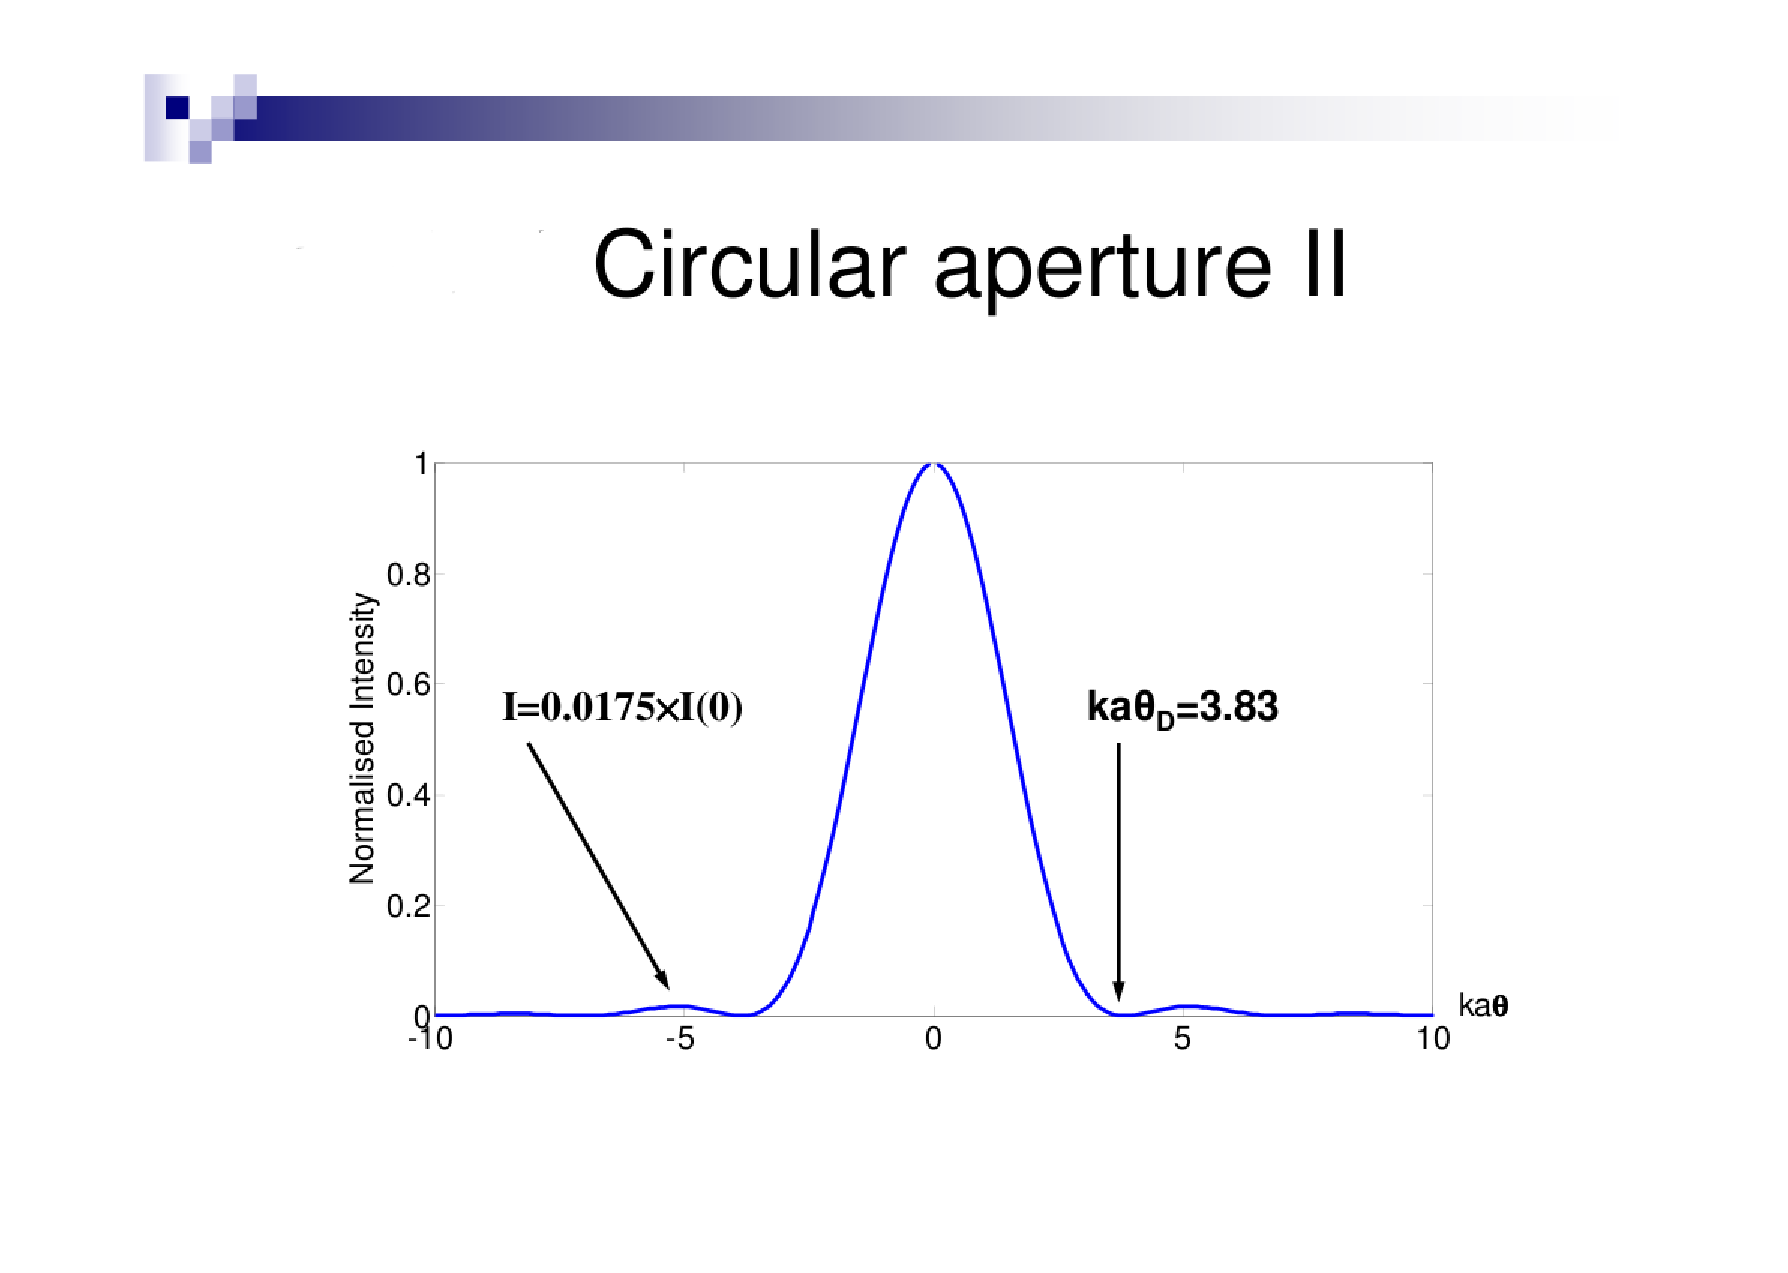
\includegraphics[scale=0.5]{circ1.eps}
\end{figure}

Edge of Airy Disc is at the first min $\theta_D$, i.e.
\begin{equation*}
3.83 = \frac{\pi d \theta_D}{\lambda}
\end{equation*}

\begin{figure}[p!]
\centering
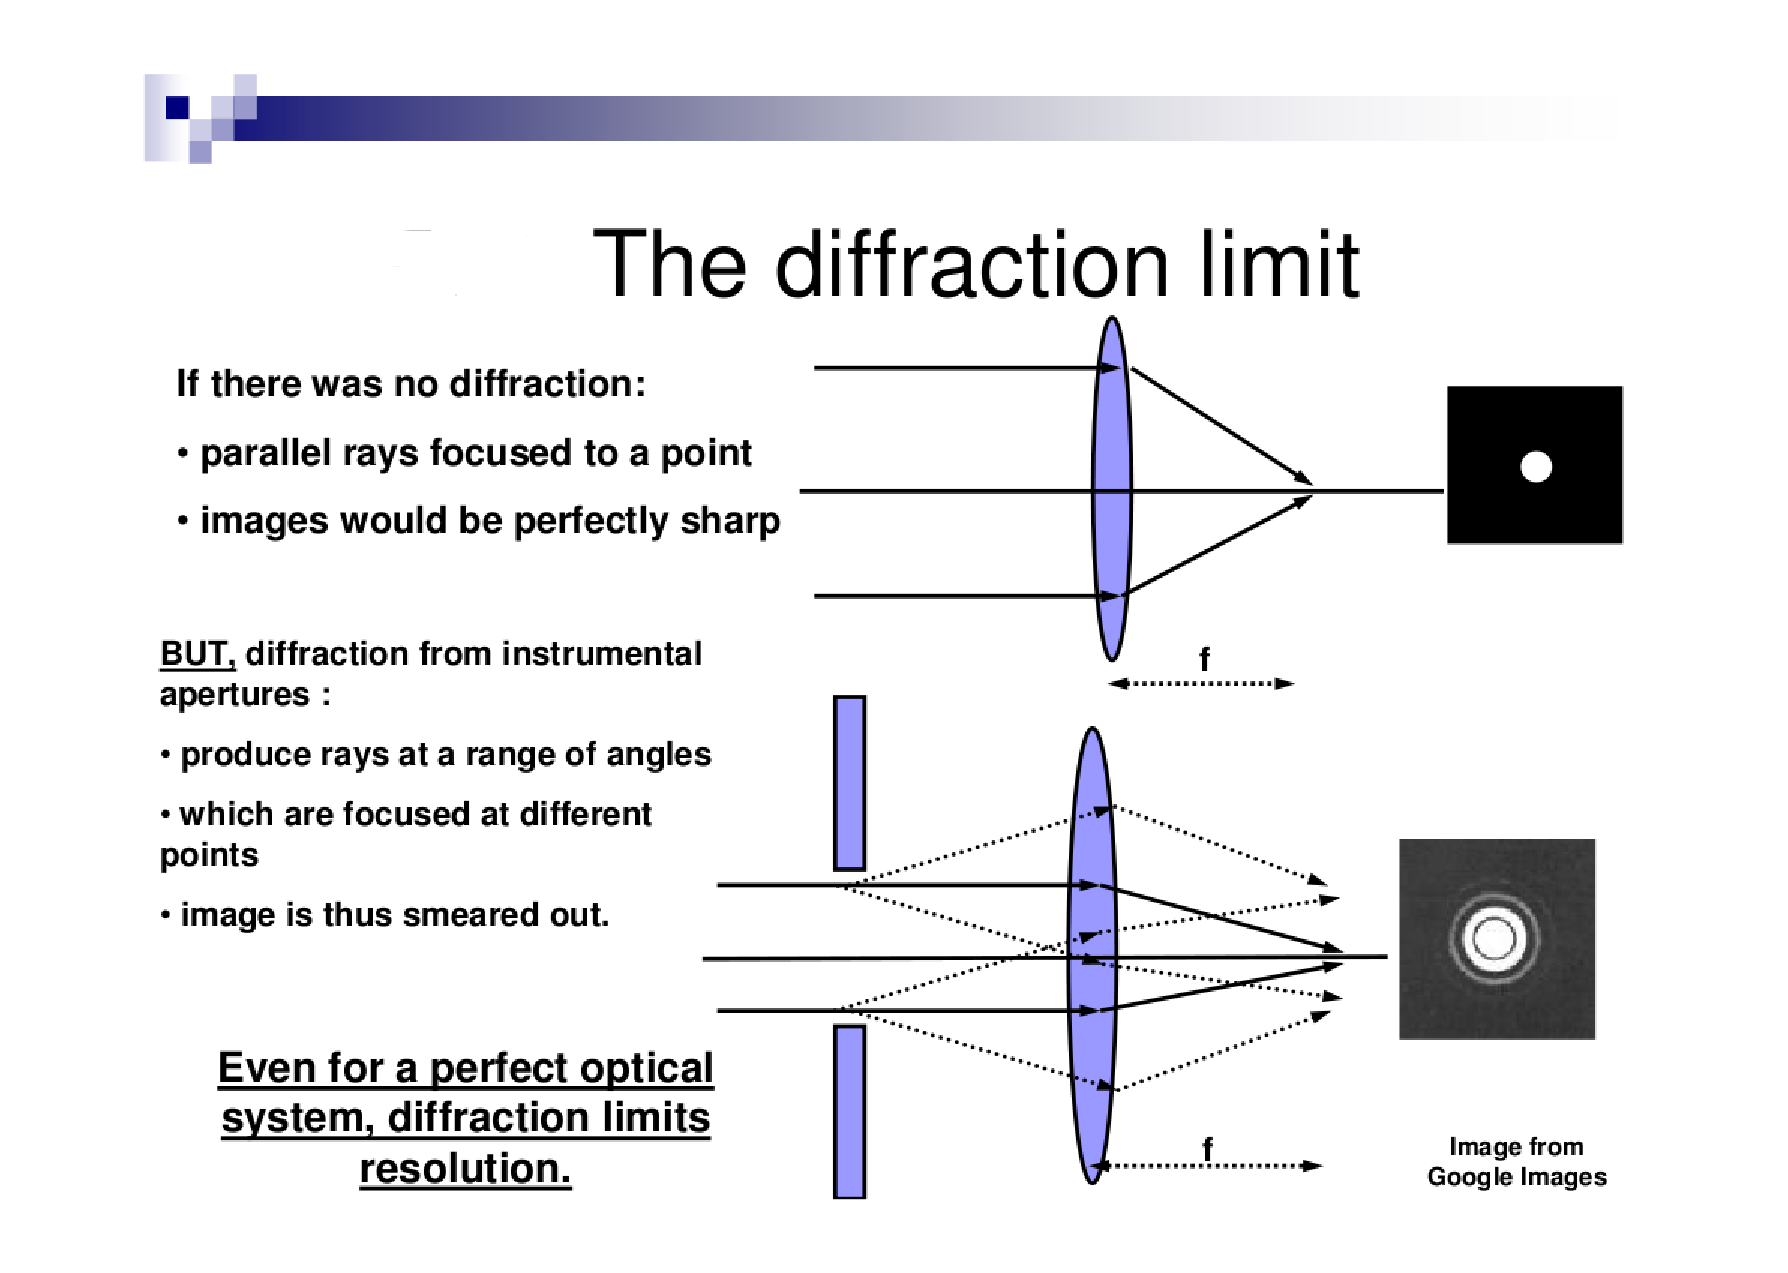
\includegraphics[scale=0.5]{circ2.eps}
\end{figure}
\begin{figure}[p!]
\centering
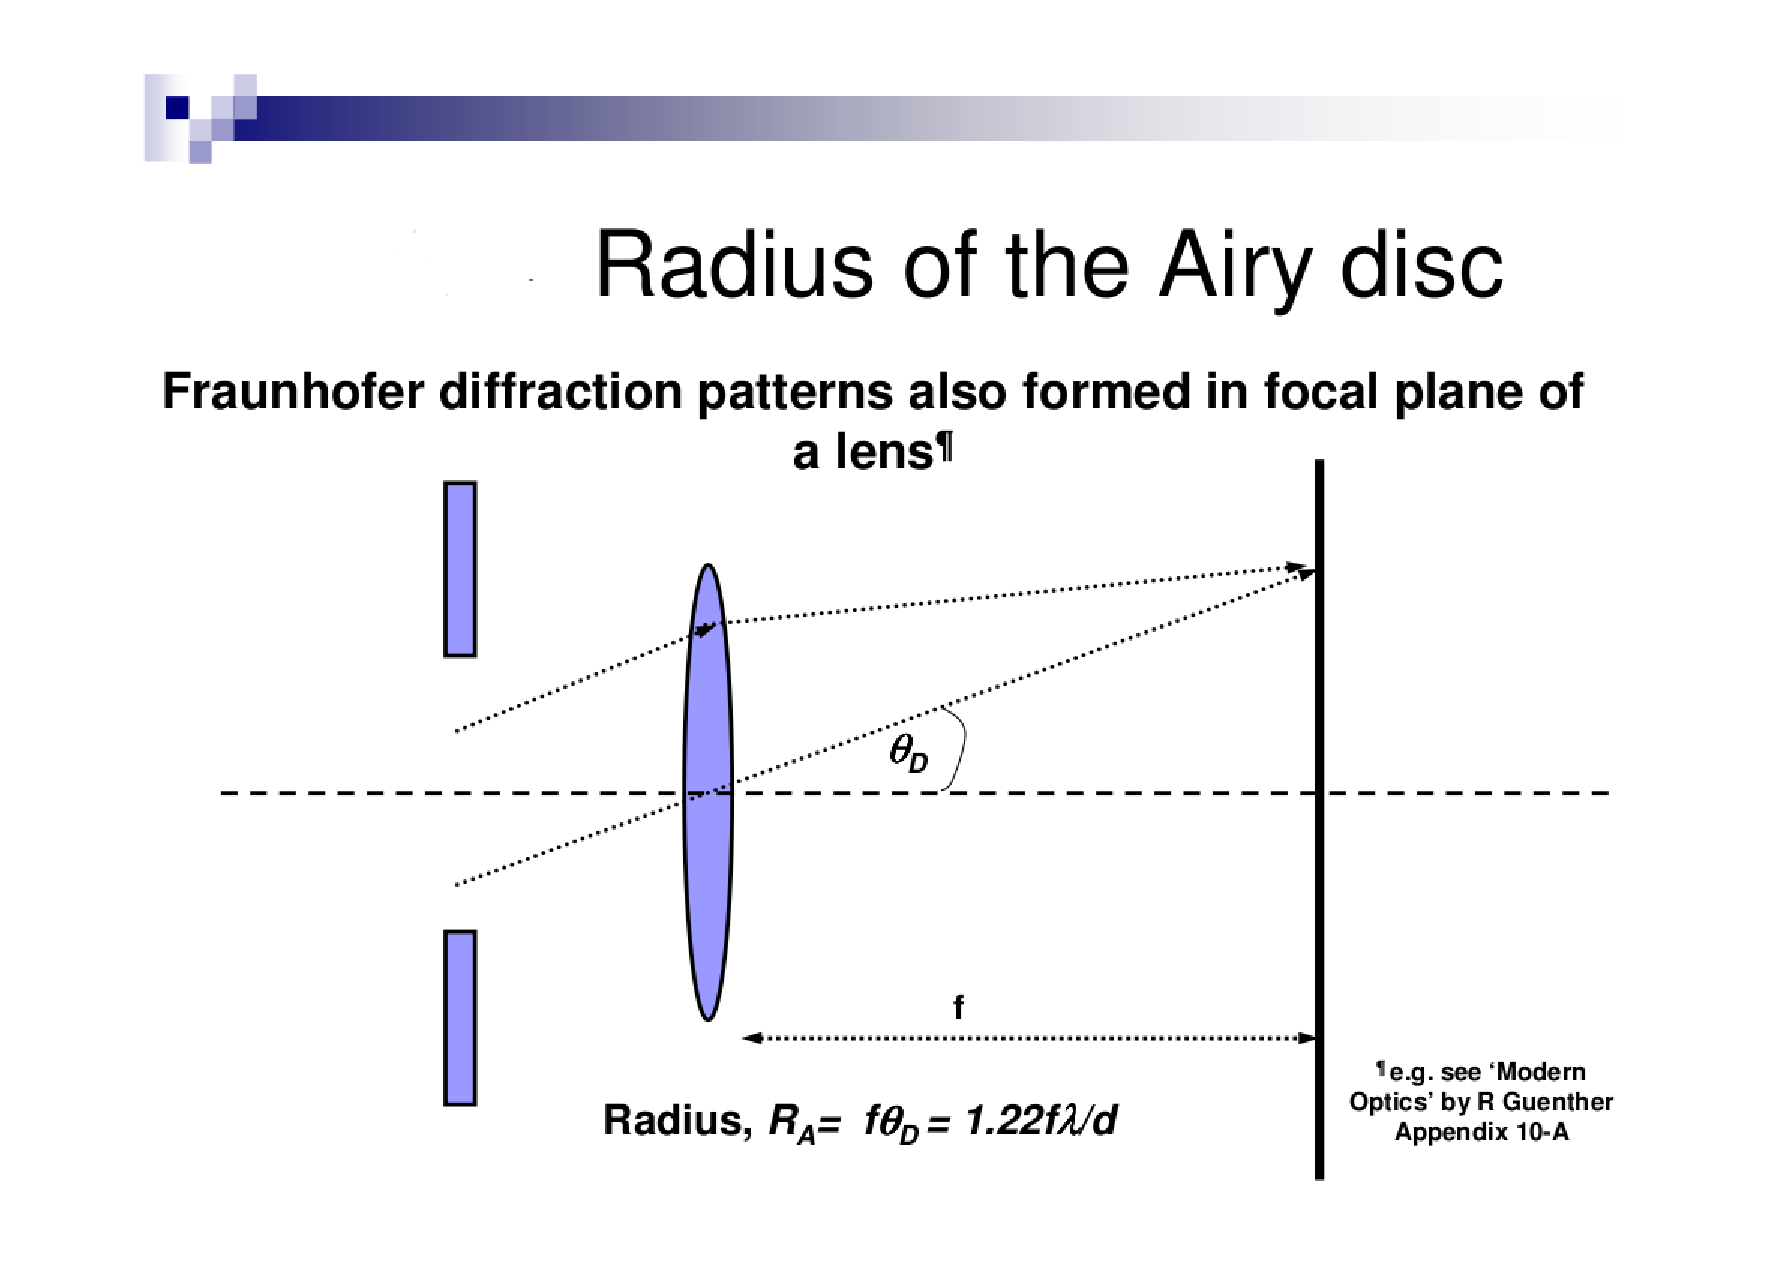
\includegraphics[scale=0.5]{circ3.eps}
\end{figure}

\begin{equation}\boxed{
\theta_D \approx 1.22\frac{\lambda}{d}
}\end{equation}

\subsubsection*{Diffraction limit}
Resolution of all optical instruments is limited by diffraction from some (usually circular) aperture (e.g. lens).

It can be shown that Fraunhofer diffraction also formed in the focal plane of a lens or mirror as well as in the far field, i.e. any linear phase variation is satisfied.

Diffraction limited angular resolution is $1.22\frac{\lambda}{d}$.

Radius of Airy disc:
\begin{equation}\boxed{
R_a = f \cdot 1.22\frac{\lambda}{d}
}\end{equation}

\subsection{Fraunhofer diffraction as Fourier Transform}
This is $2D$ Fourier Transform of aperture function $A(x,y)$.
\begin{equation*}
E(X,Y) = c F(A(x,y))
\end{equation*}
where $c$ is some constant.

Convolution:
\begin{equation}\boxed{
g(X) = \int_{-\infty} ^{\infty} f(x)h(X - x)dx
}\end{equation}
\begin{equation}\boxed{
g(X) = f(x) \ast h(x)
}\end{equation}

Convolution theorem:
\begin{equation}\boxed{
F(g) = F(f)F(h)
}\end{equation}

\subsubsection{Two thin slits}
\begin{equation*}
A_1 = \delta (x - \frac{d}{2}) + \delta (x + \frac{d}{2})
\end{equation*}
$d$ -- slit reparation.
\begin{figure}[h!]
\centering
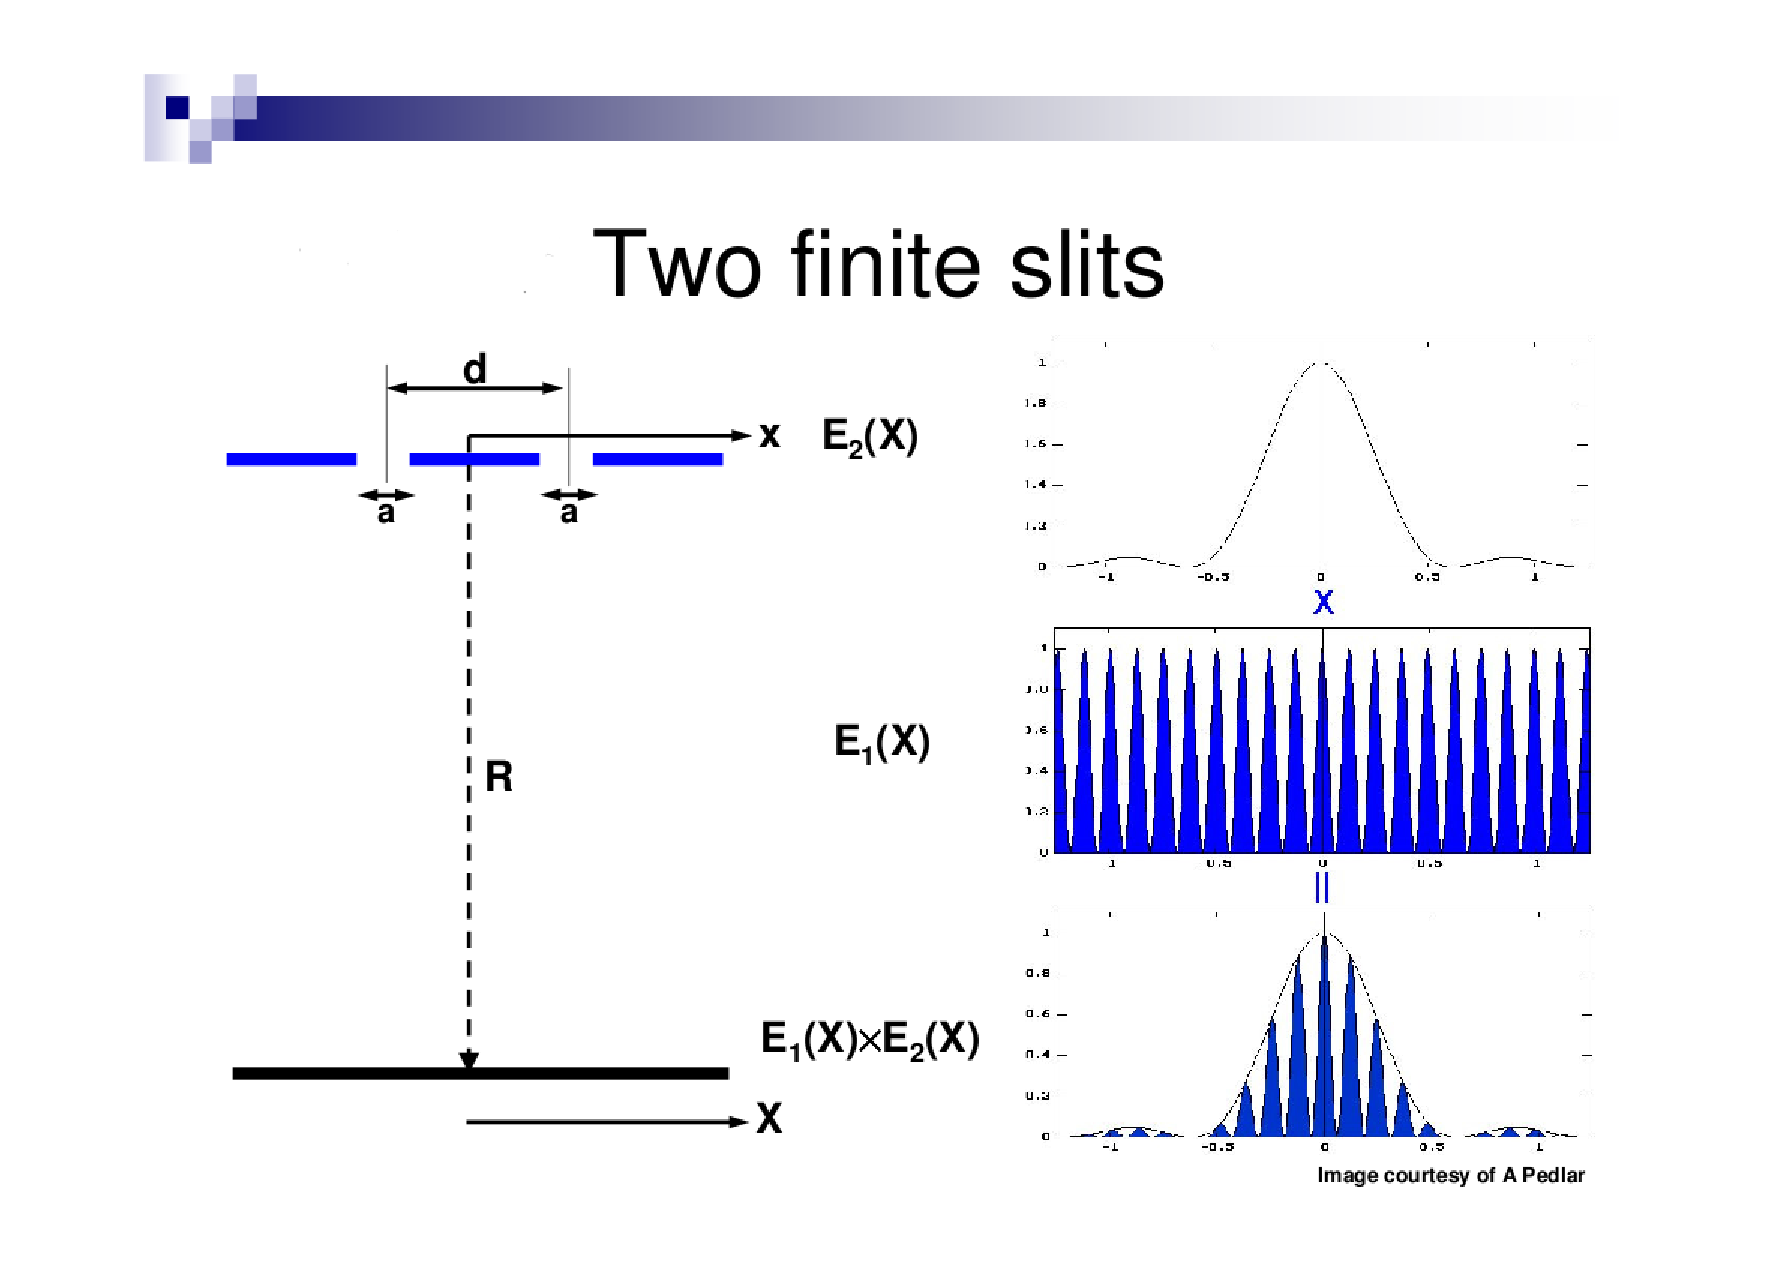
\includegraphics[scale=0.5]{R.eps}
\end{figure}
\begin{equation*}
E_1(X) = c_1 F(A_1)
\end{equation*}
\begin{flalign*}
F_1(X) & = c_1 \int_{-\infty} ^{\infty} A_1 e^{-\frac{ikxX}{R}}dx = \\
& = \frac{c_1}{2 \pi} \left[ e^{-\frac{ikdx}{2R}} + e^{\frac{ikdX}{2R}} \right] = \\
& = \frac{c_1}{\pi} \cos{\frac{kdX}{2R}} = \\
& = \frac{c_1}{\pi} \cos{\frac{\pi d X}{\lambda R}}
\end{flalign*}
\begin{equation}\boxed{
I_1 = c' \cos^2{\frac{2 \pi d X}{\lambda R}}
}\end{equation}

\subsubsection{Two thick slits}
Use convolution theorem to combine results for two thin slits and a single thick slit.
\begin{equation*}
E_2(X) = c_2 sinc{\frac{kaX}{\lambda R}}
\end{equation*}

Now
\begin{equation*}
A_2(x) \int_{-\infty} ^{\infty} A_1(x)A_2(X - x')dx' = A_1 \ast A_2
\end{equation*}
here $A_1$ stands for "two thin slits" and $A_2$ stands for "a single thick slit".
\begin{equation*}
A_1 = \delta (x - \frac{d}{2}) + \delta (x + \frac{d}{2})
\end{equation*}
\begin{equation*}
A_2 = 1
\end{equation*}
for $|x| \leq \frac{a}{2}$

Check this works:
\begin{equation*}
A_1(x') = 0
\end{equation*}
except when $x = \pm \frac{d}{2}$
\begin{equation*}
A = A_2 (x - \frac{d}{2}) + A_2(x + \frac{d}{2})
\end{equation*}
\begin{equation*}
A (x) = 1
\end{equation*}
when
\begin{equation*}
|x - \frac{d}{2}| \leq \frac{a}{2}
\end{equation*}
or
\begin{equation*}
|x + \frac{d}{2}| \leq \frac{a}{2}
\end{equation*}
\begin{equation*}
E(X) = cF(A) = cF(A_1 \ast A_2) = cF(A_1)F(A_2) = c''\cos{\frac{kdX}{2R}}sinc{\frac{kdX}{2R}}
\end{equation*}
\begin{equation}\boxed{
I(x) = I_0 \cos^2{\frac{kdX}{2R}}sinc^2{\frac{kdX}{2R}}
}\end{equation}

\subsubsection{Point pread function (PSF)}
PSF is response of an optical system to a point-source of light (blurring or smearing). Regard object as an array of point sources.
\begin{figure}[h!]
\centering
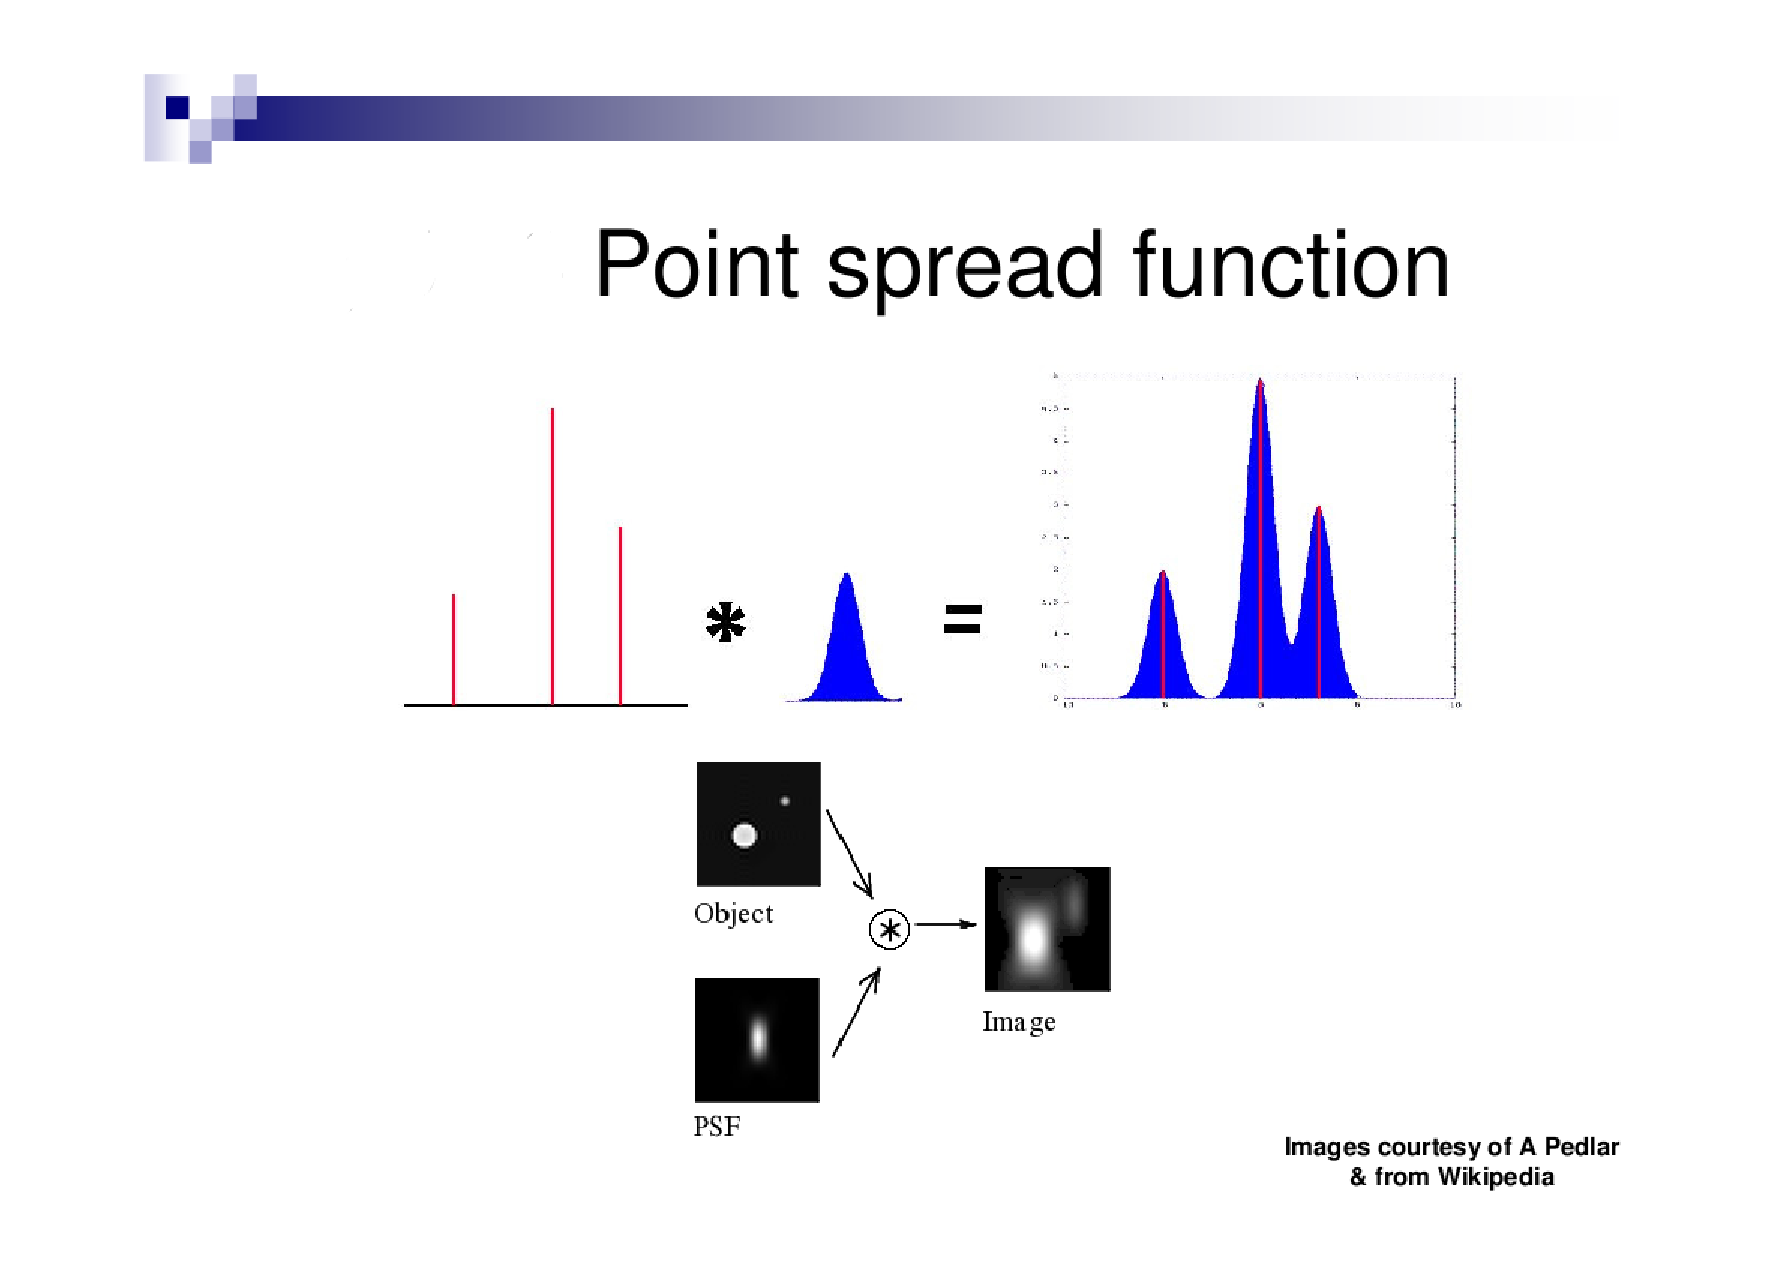
\includegraphics[scale=0.5]{image.eps}
\end{figure}
\begin{equation*}
Image = PSF \ast Object
\end{equation*}

If you know $PSF$, find $F(PSF)$.
\begin{equation*}
F(Image) = F(PSF)F(Object)
\end{equation*}
\begin{equation*}
F(Object) = \frac{F(Image)}{F(PSF)}
\end{equation*}
\begin{equation*}
Object = F^{-1}\left(\frac{F(Image)}{F(PSF)}\right)
\end{equation*}
this process is called deconvolution.

\subsection{Diffraction gratings}
\begin{figure}[p!]
\centering
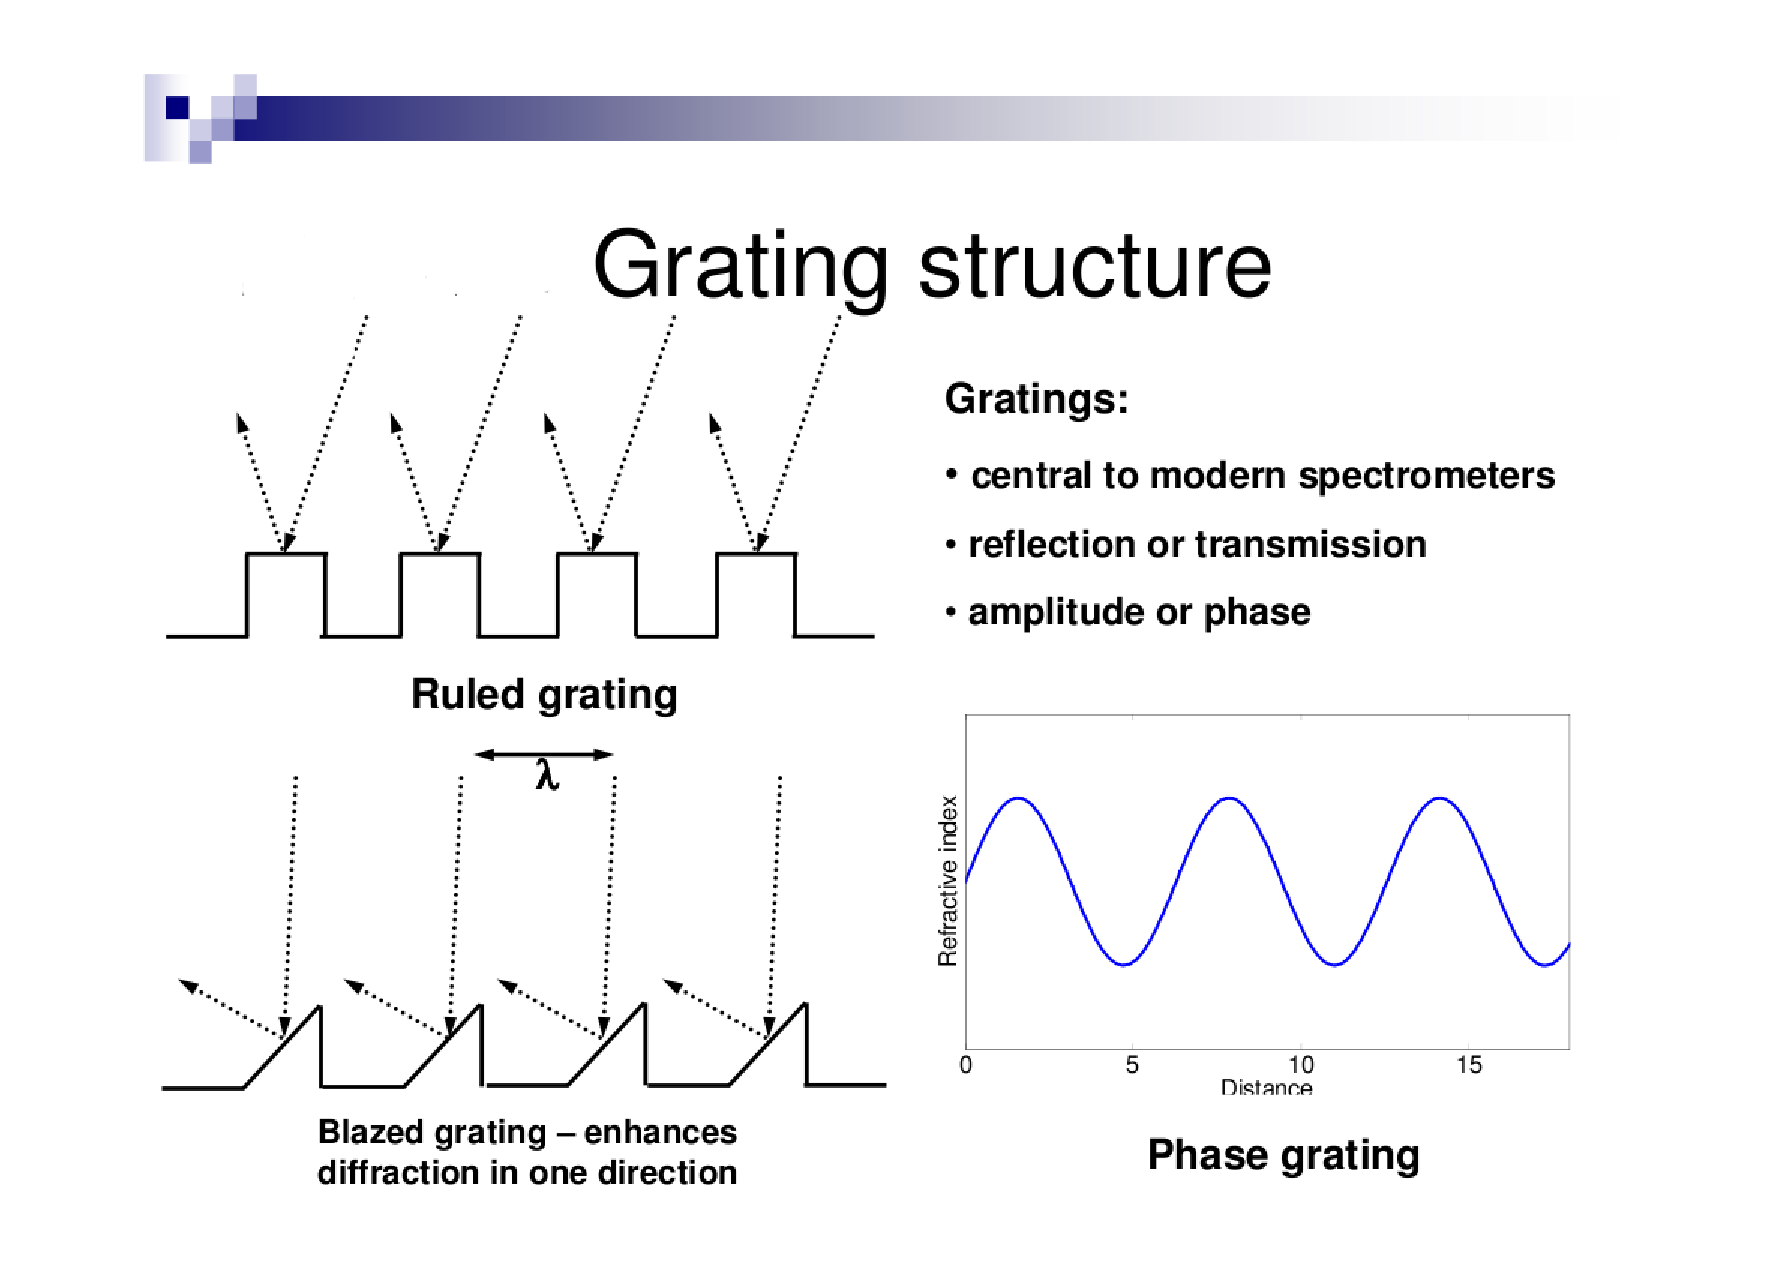
\includegraphics[scale=0.5]{grating.eps}
\end{figure}
\begin{figure}[p!]
\centering
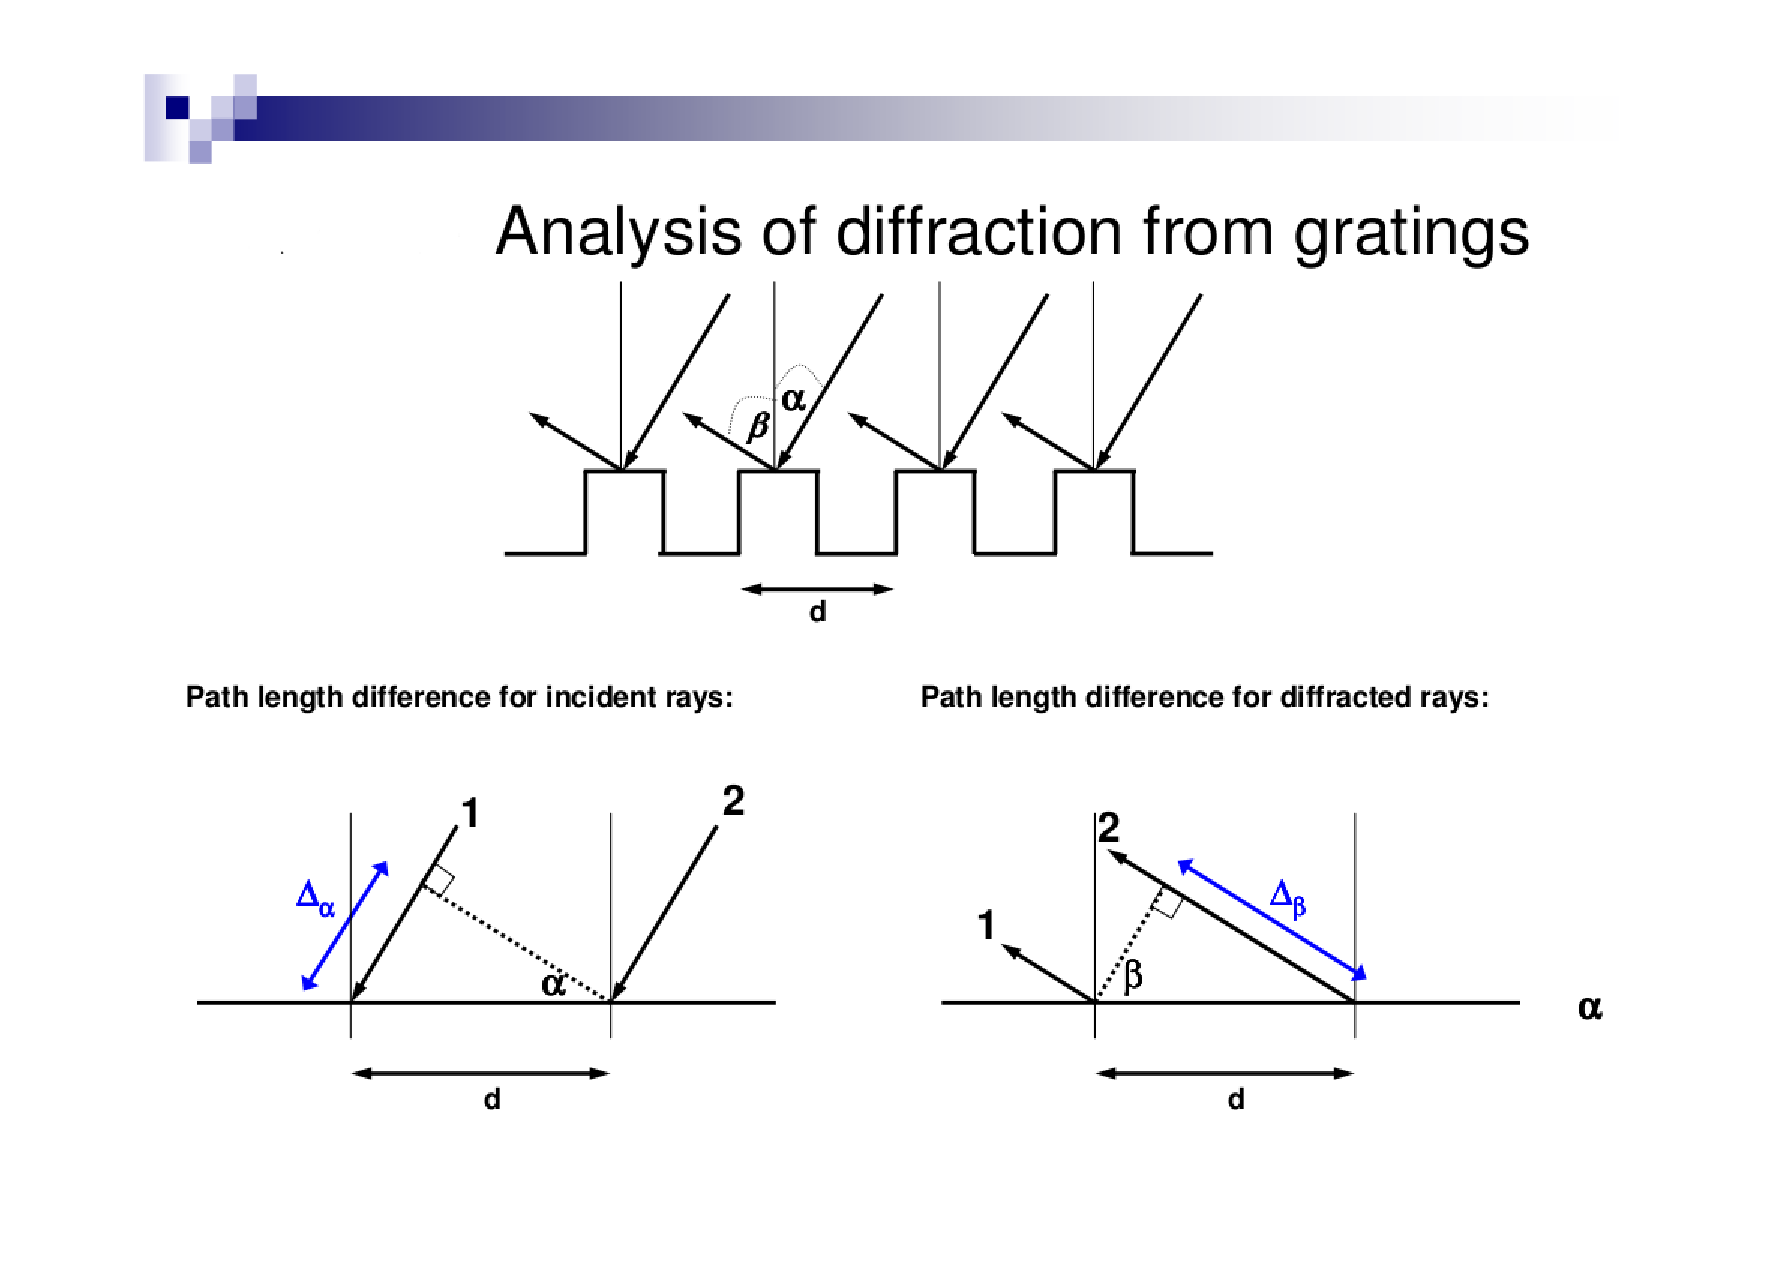
\includegraphics[scale=0.5]{grating1.eps}
\end{figure}

Path length diffrence (pld) for incident rays:
\begin{equation*}
\Delta_\alpha = d \sin{\alpha}
\end{equation*}

Pld for diffracted rays:
\begin{equation*}
\Delta_\beta = - d \sin{\beta}
\end{equation*}

Total pld:
\begin{equation*}
\Delta_\alpha  + \Delta_\beta = d (\sin{\alpha} - \sin{\beta})
\end{equation*}

Diffraction maxima occure when
\begin{equation*}
pld = m \lambda
\end{equation*}
where $m$ is integer.
\begin{equation}\boxed{
m \lambda = d (\sin{\alpha} - \sin{\beta})
}\end{equation}
this is known as grating equation.

For $m = 0$, $\alpha = \beta$ -- reflection.

For $m \neq 0$, $\beta = f(\lambda)$. Use the separate wavelength.

\subsection{Frensel diffraction}
Recall general diffraction equation:
\begin{equation}\boxed{
E(P) = \epsilon' \frac{e^{iks}}{s}\int \int K(\alpha) \frac{e^{ikr}}{r}dA
}\end{equation}

Fraunhofer diffraction (far field):
\begin{itemize}
\item[(i)] $K(\alpha) \approx 1$
\item[(ii)] $r \approx R$ in denominator.
\end{itemize}

Frensel diffraction (near field):
\begin{itemize}
\item[(i)] $K(\alpha) = \frac{1}{2}(1 + \cos{\alpha})$
\item[(ii)] $r \neq R$ in denominator
\end{itemize}
\begin{equation}\boxed{
E(P) = \frac{\epsilon}{2} \int \int (1 + \cos{\alpha}) \frac{e^{ikr}}{r}dA
}\end{equation}
\begin{equation*}
\epsilon = \frac{\epsilon' e^{iks}}{s}
\end{equation*}
$r \neq$ linear function of $x$ and $y$.

This equation is solvable in general.

\subsubsection{Circular obstructions}
For circular symmetric aperture Frensel diffraction can be analysed to a good approximation by using an idea of "half-period" or "Frensel zones".
\begin{figure}[h!]
\centering
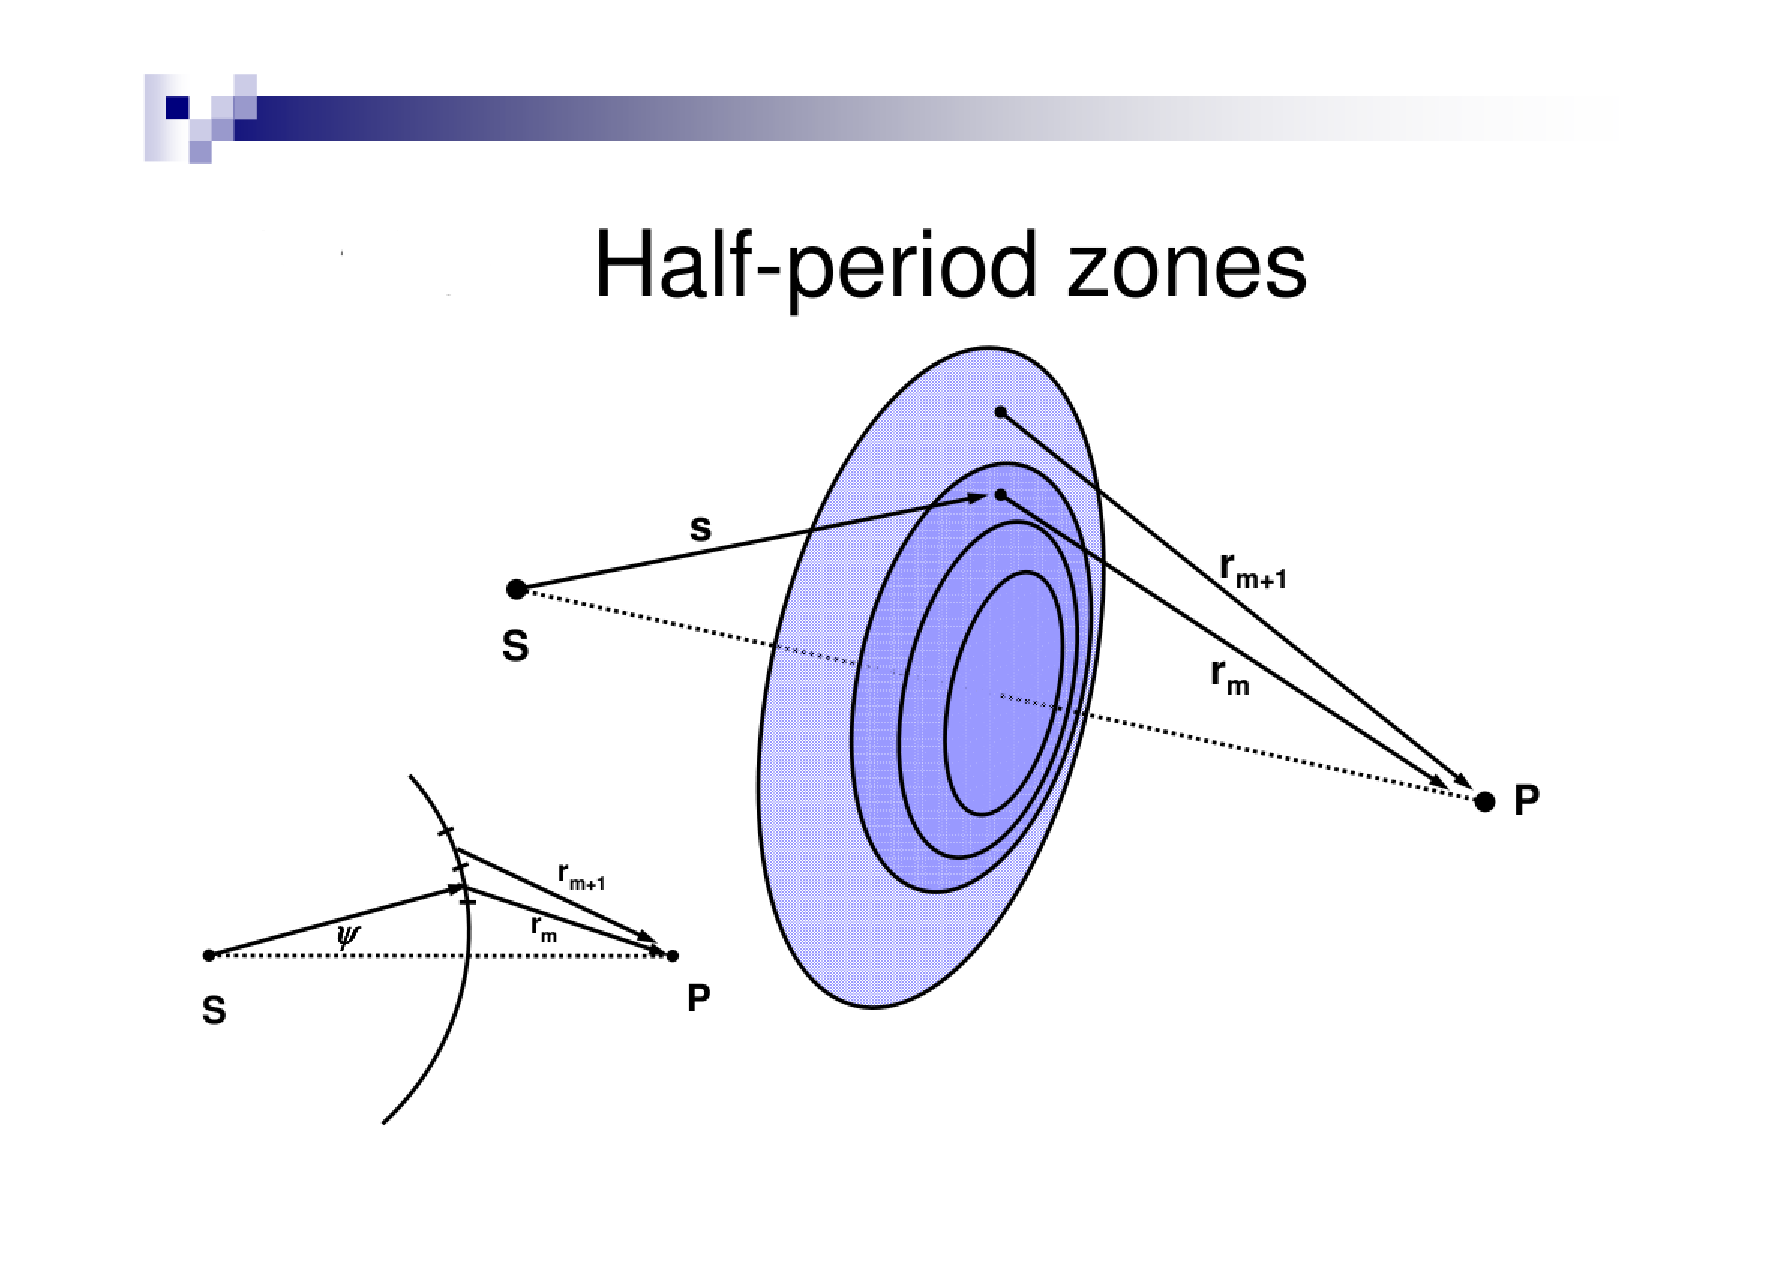
\includegraphics[scale=0.5]{zone.eps}
\end{figure}

Zone $Z_m$ is
\begin{itemize}
\item ring-shaped part of a spherical wavefront;
\item $\frac{m \lambda}{2}$ further away from $P$ than nearest point.
\end{itemize}

Approximations:
\begin{itemize}
\item[(i)] all wavelets in a zone are in phase;
\item[(ii)] $K(\alpha) \approx const$ over a zone.
\end{itemize}

Therefore field at $P$ due to $m^{th}$ zone:
\begin{equation*}
E_m(P) = \epsilon K_m \frac{e^{ikz_m}}{z_m}\int \int_{zone} dA
\end{equation*}

Area of $m^{th}$ zone:
\begin{figure}[h!]
\centering
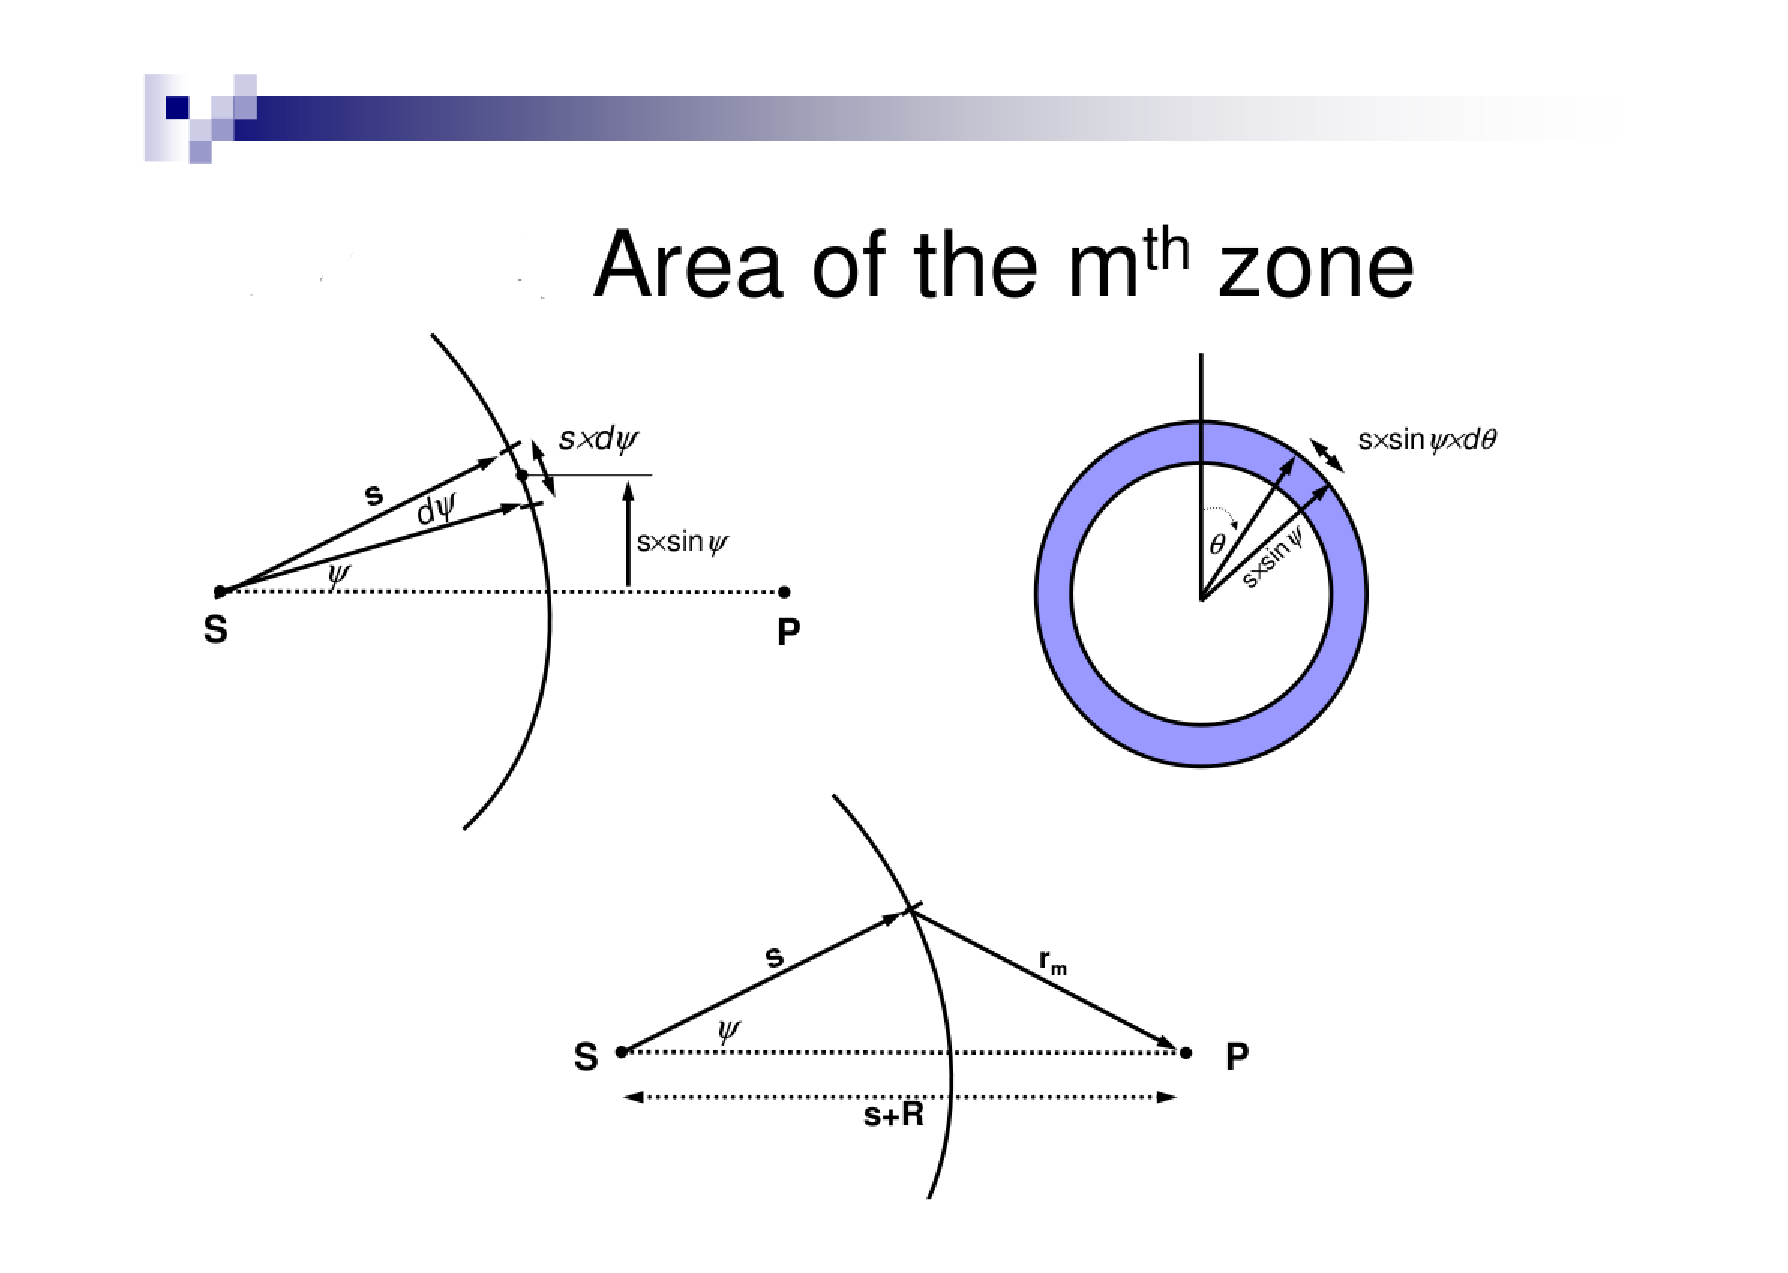
\includegraphics[scale=0.5]{area.eps}
\end{figure}
\begin{equation*}
dA = sd\psi s \sin{\psi} d \theta
\end{equation*}
cosine rule:
\begin{equation*}
r^2_m = s^2 + (s + R)^2 - 2s(s+R)\cos{\psi}
\end{equation*}

Differentiate w.r.t $r_m$:
\begin{equation*}
2r_m = 2s(s + R)\sin{\psi}\frac{d\psi}{dr_m}
\end{equation*}
therefore
\begin{equation*}
s \sin{\psi} d\psi = \frac{r_m dr_m}{s+R}
\end{equation*}
\begin{equation*}
dA = \frac{sr_m d r_m d \theta}{s+R}
\end{equation*}
\begin{equation*}
A = \int_0^{2\pi} \int_{R + \frac{m \lambda}{2}}^{R + \frac{(m+1) \lambda}{2}} \frac{sr_m d r_m}{s+R}d\theta
\end{equation*}
\begin{equation*}
A = \frac{2 \pi s}{s+R} \left(R\lambda +\frac{\lambda^2}{4}(2m +1)\right)
\end{equation*}
for $m \lambda << R$
\begin{equation}\boxed{
A_m = \frac{\pi s}{s+R}R\lambda
}\end{equation}
\begin{equation*}
A_m \neq f(m) 
\end{equation*}
$\Rightarrow$ all zones have equal area. Now
\begin{equation*}
E_m(P) = \epsilon \frac{K_m}{r_m}\frac{\pi s}{s + R}R \lambda
\end{equation*}

Consider $\frac{E_{m+1}}{E_m}$:
\begin{equation*}
\frac{E_{m+1}}{E_m} = \frac{K_{m+1}}{K_m} \frac{r_m}{r_{m+1}}e^{ik(r_m - r_{m+1})}
\end{equation*}
but $K_{m+1} \approx K_m$ and $r_m - r_{m+1} = \frac{\lambda}{2}$
\begin{equation*}
\frac{E_{m+1}}{E_m} = e^{\frac{ik\lambda}{r}} = e^{i\pi} = -1
\end{equation*}
\begin{equation*}
E_{max} = - E_m
\end{equation*}

Adjacent zones cancell out.

For a circular aperture of area $A_a$ the number of zones $N = \frac{A_a}{A_z}$.

If $N$ is even integer, then $E(P) = 0$ -- min.

If $N$ is odd integer, then $E(P) = E_m$ -- max.

In general:
\begin{equation*}
0 \leq E(P) \leq E_m
\end{equation*}

Black altonode zones $\Rightarrow$ just constructive interference ($2\pi$ phase difference between zones) $\Rightarrow$ zone plate $\Rightarrow$ focus length.

\subsubsection{Straight edge}
Without circular symmetry, it's very difficult/impossible to solve H.F.I., except in special cases, when $s_0, R >>$ aperture. Set $s,r \approx const$ in denominator $\Rightarrow$
\begin{itemize}
\item[(i)] $K \approx 1$
\item[(ii)] $x,y << R$
\end{itemize}
\begin{figure}[h!]
\centering
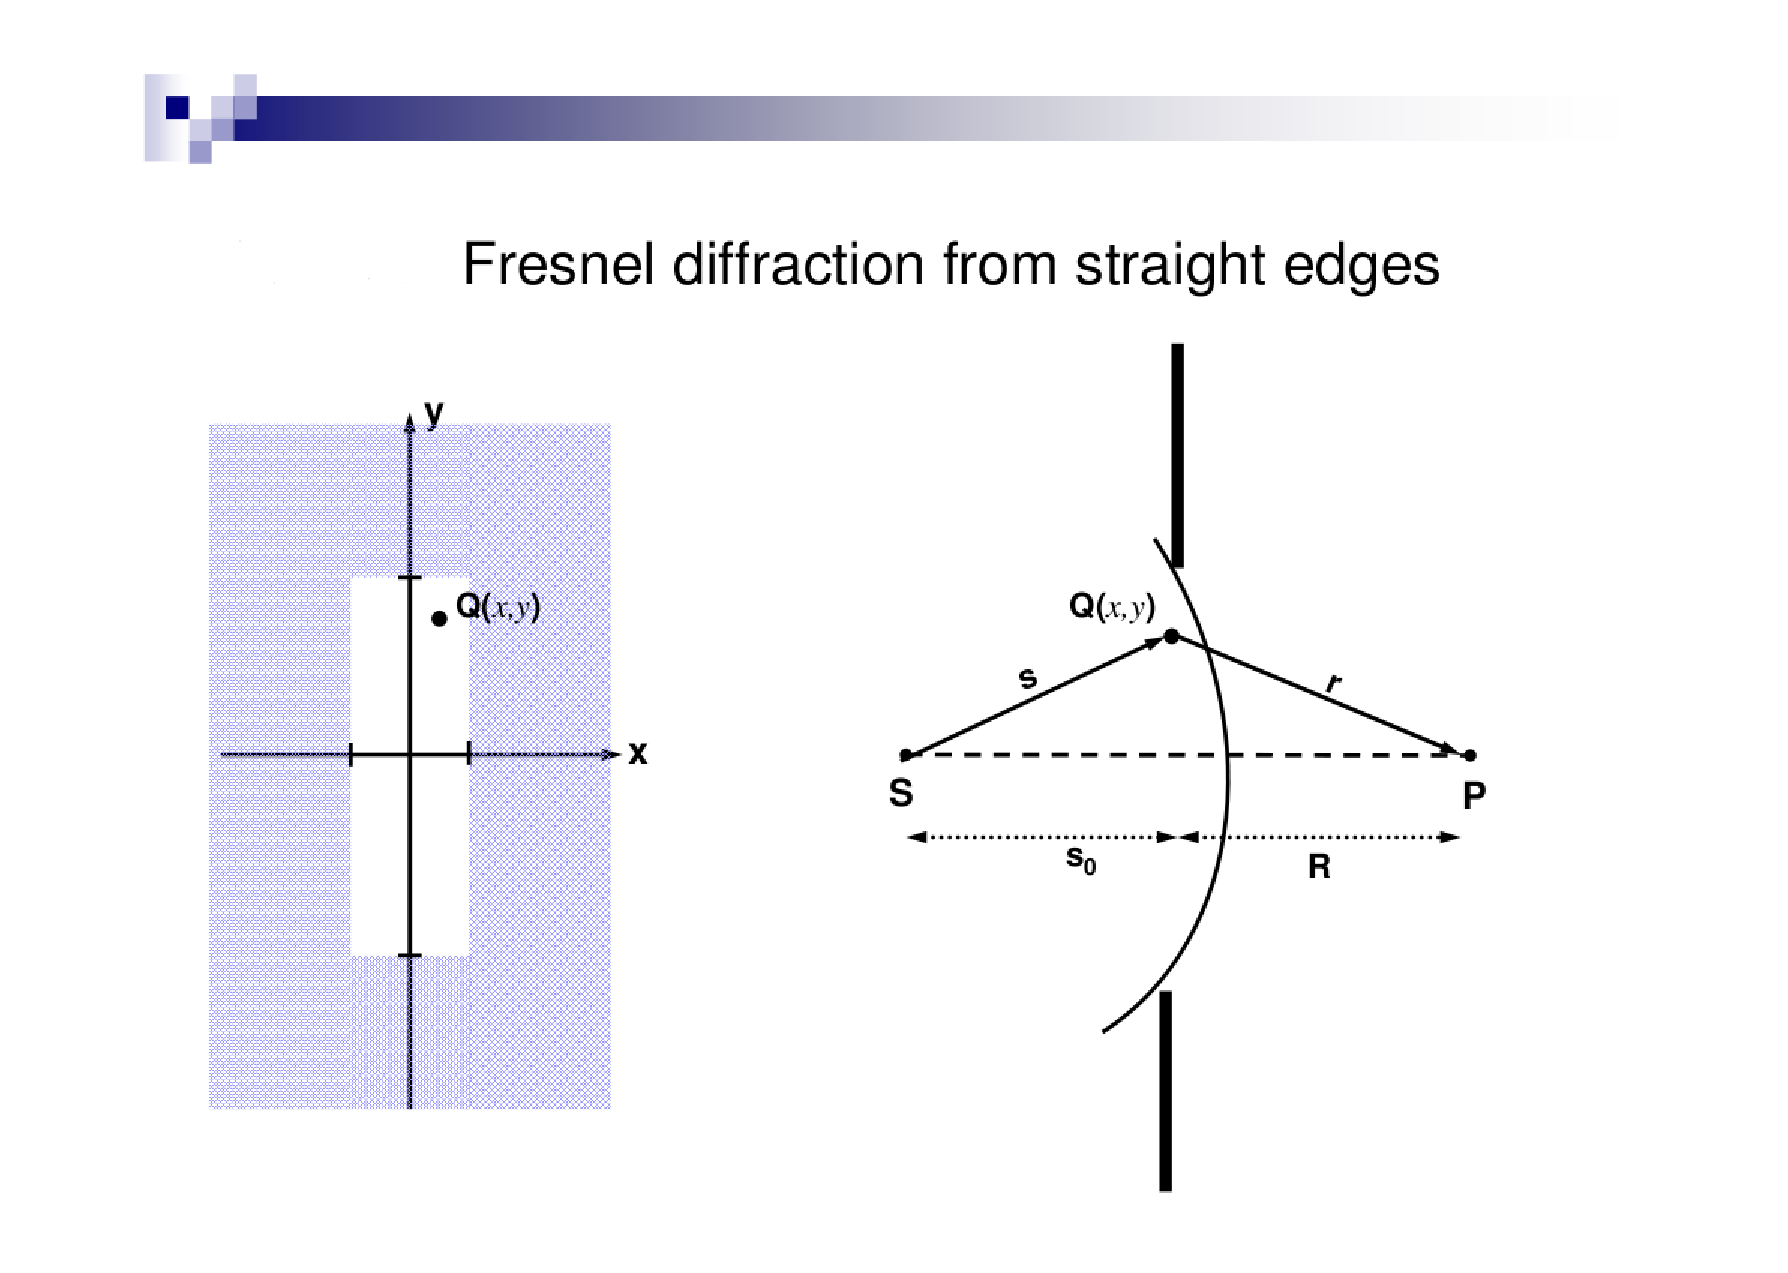
\includegraphics[scale=0.5]{s.eps}
\end{figure}

Fraunhofer diffraction also assumes $x,y << X,Y , s = const \approx s_0$.

Now phase is not a linear function of $x$ and $y$.

HFI:
\begin{equation*}
E(P) = \frac{\epsilon'}{s_0 R}\int \int_{aperture} e^{ik(r + s)}dA
\end{equation*}
\begin{equation*}
s^2 = s_0^2 + x^2 + y^2
\end{equation*}
\begin{equation*}
r^2 = R^2 + x^2 + y^2
\end{equation*}

Binominal expansion:
\begin{equation*}
s \approx s_0 + \frac{x^2 + y^2}{2s_0}
\end{equation*}
\begin{equation*}
r \approx R + \frac{x^2 + y^2}{2R}
\end{equation*}
\begin{equation*}
s + r = s_0 + R + (x^2 + y^2)\frac{s_0 + R}{s_0 R}
\end{equation*}
\begin{equation}\boxed{
E(P) = \frac{\epsilon'}{s_0 R}e^{ik(s_0 + R)}\int e^{\frac{ik(s_0 + R)x^2}{2s_0R}} dx \int e^{\frac{ik(s_0 + R)y^2}{2s_0R}}dy
}\end{equation}
these integrals are Frensel integrals.

\section{Lasers}
\subsection{Absorbtion and emission in atomic systems}
\begin{figure}[h!]
\centering
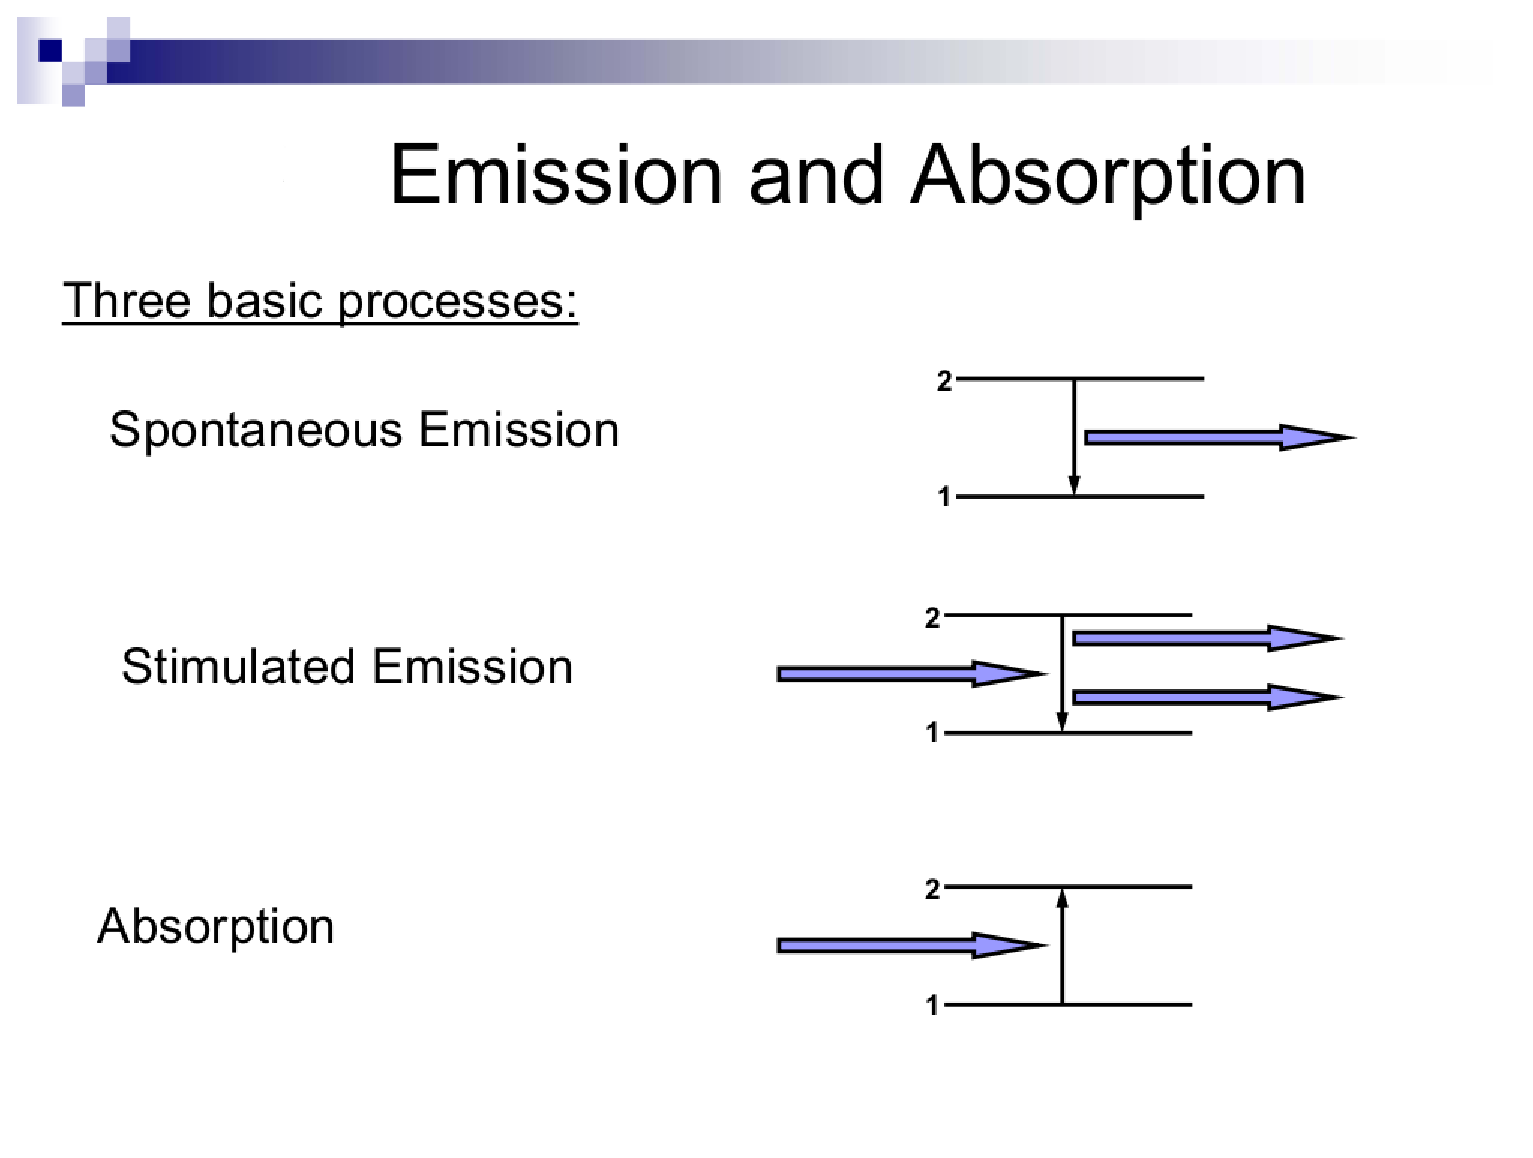
\includegraphics[scale=0.5]{laser1.eps}
\end{figure}
Spontaneous emission:
\begin{equation*}
\frac{dN_2}{dt} = -N_2 A_{21}
\end{equation*}
$A_{21}$ -- Einstein A coefficient.
\begin{equation*}
A_{21} = \frac{1}{\tau_{12}}
\end{equation*}
$\tau_{12}$ -- lifetime of a process.

Stimulated emission
\begin{equation*}
\frac{dN_2}{dt} = - N_2 B_{21}\rho
\end{equation*}

Energy density:
\begin{equation*}
\rho = \frac{E}{c}
\end{equation*}
$B_{21}$ -- Einstein B coefficient for stimulated emission.

Absorbtion:
\begin{equation*}
\frac{dN_1}{dt} = - N_1 B_{12} \rho
\end{equation*}
$B_{12}$ -- Einstein B coefficient for absorbtion.

Therefore rate equation for level 2:
\begin{equation*}
\dot{N_2} = -N_2 B_{21} \rho - A_{21}N_2 + N_1 B_{12}\rho
\end{equation*}

Consider what happens in thermal equuilibrium:
\begin{itemize}
\item[(i)] $\dot{N_2} = 0$
\item[(ii)] Energy density is that of a black body:
\begin{equation*}
\rho(\nu) = \frac{8\pi h \nu^3}{c^3}\frac{1}{e^{\frac{h \nu}{kT}} - 1}
\end{equation*}
\item[(iii)] Thermal property of energy levels:
\begin{equation*}
\frac{N_2}{N_1} = e^{-\frac{h \nu}{kT}}
\end{equation*}
\end{itemize}

Rate equation becomes:
\begin{equation*}
\frac{8\pi h \nu^3}{c^3}\frac{1}{e^{\frac{h \nu}{kT}} - 1} = \frac{A_{21}}{B_{12}e^{\frac{h \nu}{kT}} - B_{21}}
\end{equation*}
\begin{equation*}
B_{12} = B_{21} = B
\end{equation*}
\begin{equation*}
\frac{A_{21}}{B} = \frac{8 \pi h \nu^3}{c^3}
\end{equation*}

For a degenerate system
\begin{equation*}
g_1 B_{12} = g_2 b_{21}
\end{equation*}
$g_i$ -- number of degenerate states on $1^{st}$ level.

\subsection{Optical gain and population invertion}
\begin{figure}[h!]
\centering
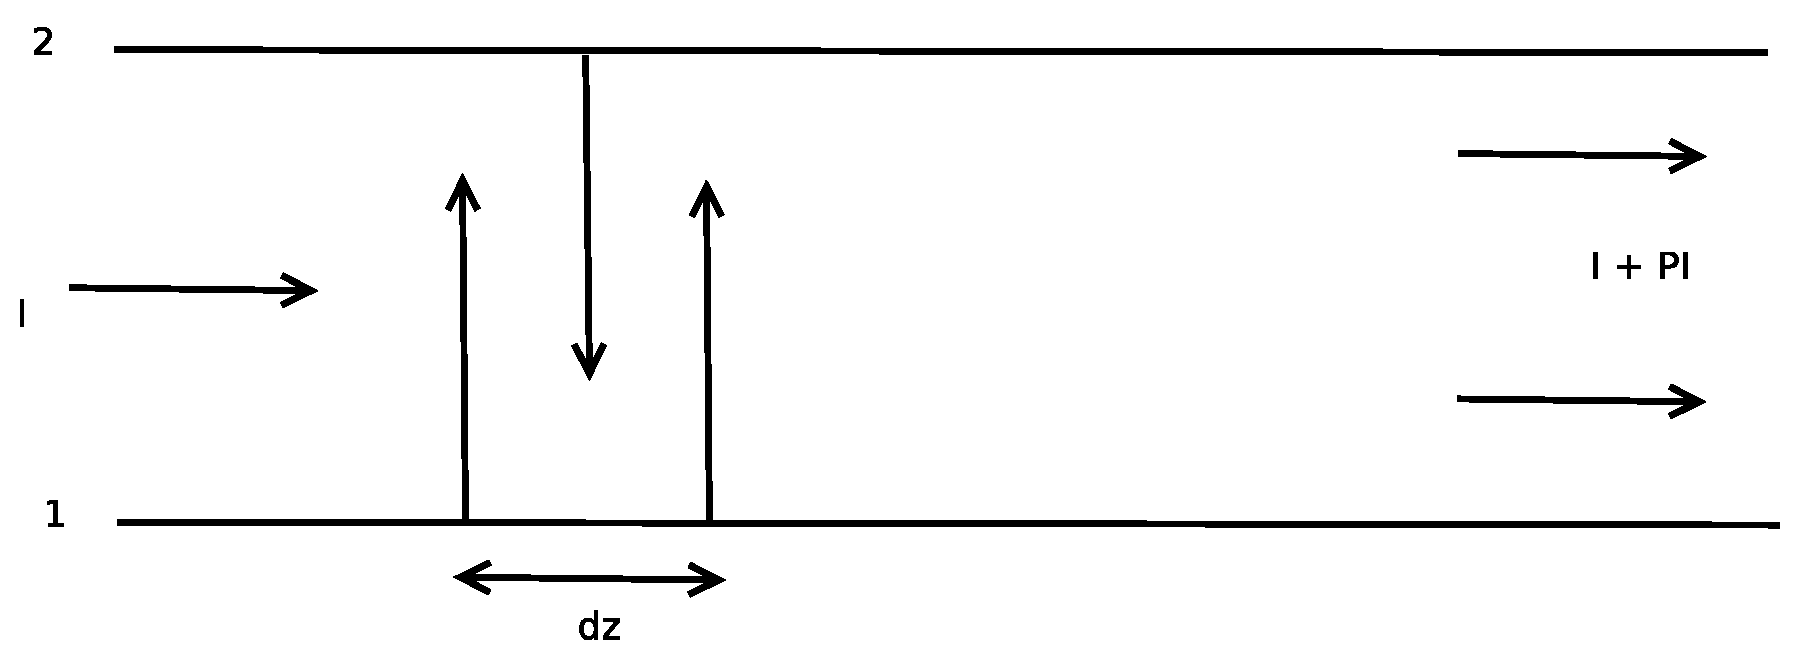
\includegraphics[scale=0.5]{gain.eps}
\end{figure}
\begin{equation*}
\delta I = \left({\# stim.emissions p.v.} - {\# absorb. p.v.} \right) h \nu \delta z = \left(N_2 B_{21}\frac{I}{c} - N_1 B_{12}\frac{I}{c} \right) h \nu \delta z
\end{equation*}
\begin{equation*}
\frac{dI}{dz} = \frac{(N_2 - N_1)BIh\nu}{c}
\end{equation*}
$N_2 - N_1$ -- population
\begin{equation*}
\frac{dI}{dz} > 0
\end{equation*}
if $N_2 > N_1 \Rightarrow$
population inversion.
\begin{equation*}
I(z) = I_0(0)e^{\gamma z}
\end{equation*}
is optical gain, where $\gamma$ is gain coefficient.
\begin{equation*}
\gamma = \frac{N_2 - N-1}{c}B h \nu
\end{equation*}
\begin{equation*}
\gamma = (N_2 - N_1)\sigma = N \sigma
\end{equation*}
$\sigma$ -- stimulated emission cross section \\
$N$ -- population inversion.

But for thermal population distribution $N_2 < N_1$, therefore need to excite or "pump" the gain medium to get a population inversion (typically, with another light source or by electric current).

Now rate equation:
\begin{equation*}
\dot{N_2} = - N_2 B_{21} \rho - A_{21}N_2 + N_1 B_{12} \rho + R
\end{equation*}
where $R$ is pump rate, i.e. rate of excitation to level 2.

Now have an optical amplifier if we pump at a sufficiently high rate such that $N_2 - N_1 > 0$.

\subsection{Thershold and steady state operation}
\begin{figure}[h!]
\centering
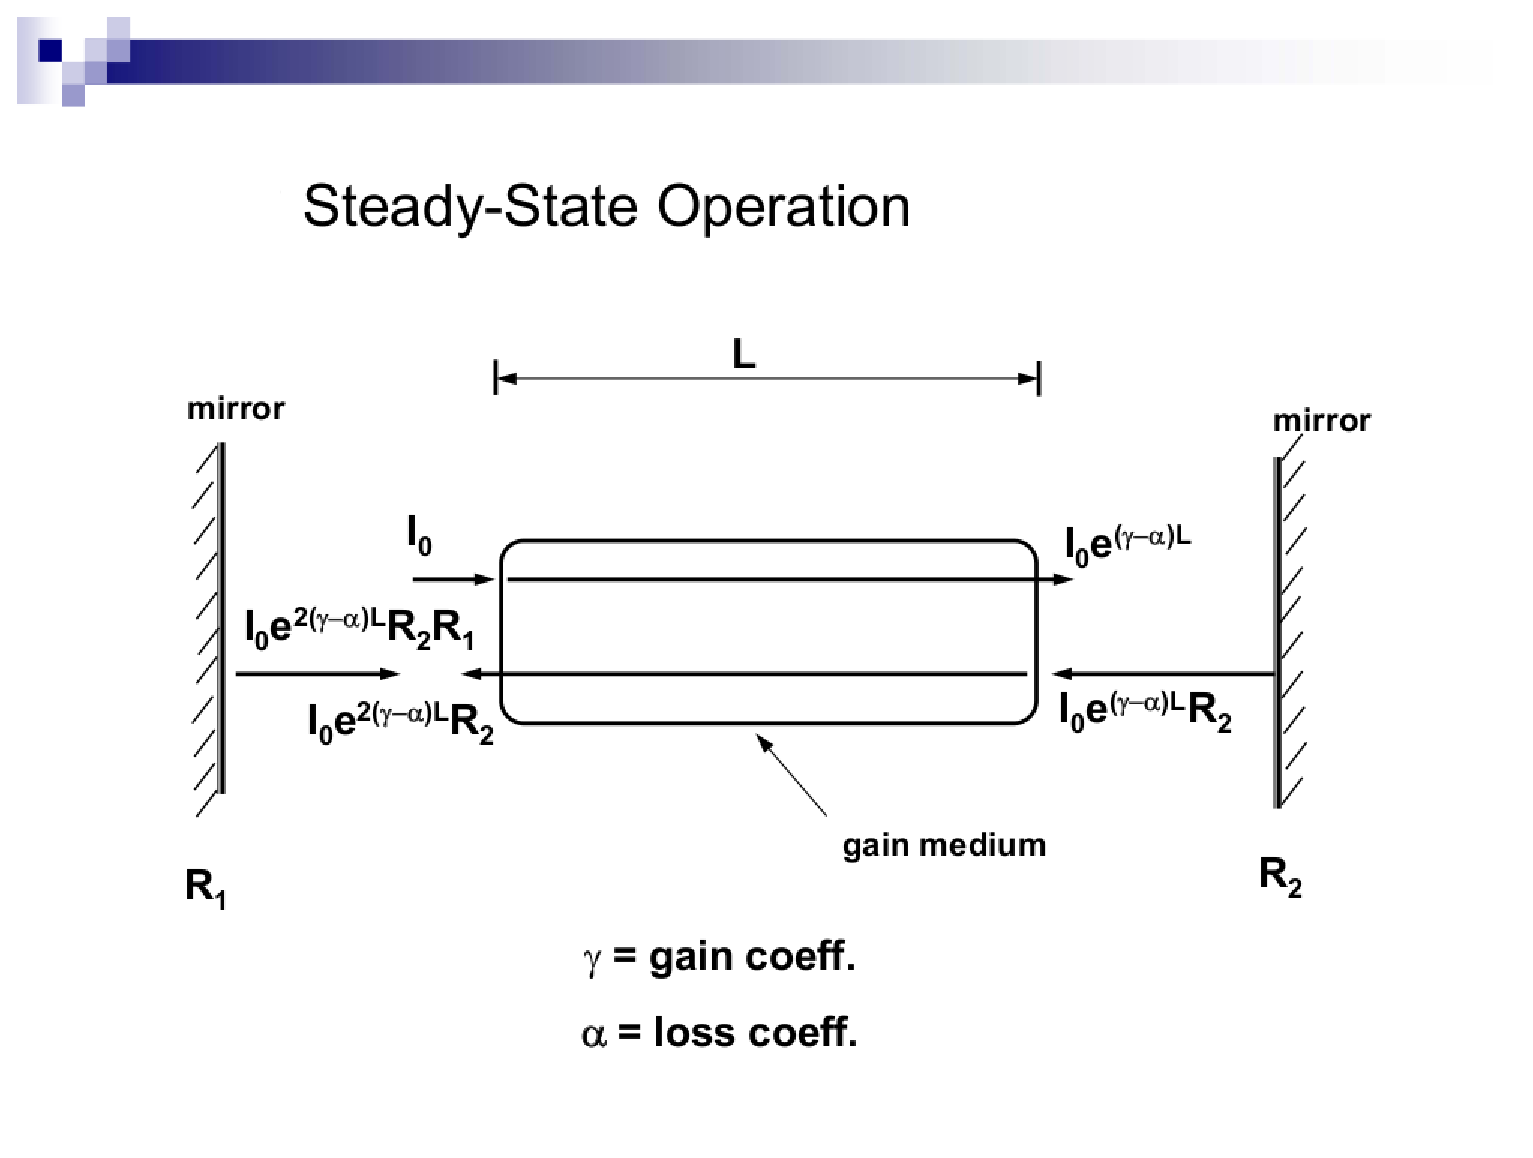
\includegraphics[scale=0.5]{laser2.eps}
\end{figure}
Intensity after round trip in cavity
\begin{equation*}
I_{RT} = I_0 R_1 R_2 e^{2(\gamma - \alpha)L}
\end{equation*}
where $\alpha$ -- loss coefficient\\
$L$ -- length of gain mechanism\\
$R_1, R_2$ -- mirror reflectances.

For a steady state:
\begin{equation*}
I_{RT} = I_R = R_1 R_2 e^{2(\gamma_{TH} - \alpha)L}
\end{equation*}
where $\gamma_{TH}$ is "\textit{thershold gain coefficient}".
\begin{equation*}
\gamma_{TH} = \alpha - \frac{1}{2L} \ln{(R_1 - R_2)}
\end{equation*}

If $N$ is such that $\gamma > \gamma_{TH}$, then $I$ goes up at rate of the stimulated emission increases until $N$ goes down to where $\gamma = \gamma_{TH}$ again, i.e. $N=N_{TH}$ is a steady state which mainains but at higher intensity.

\subsection{4-level lasers}
\begin{figure}[h!]
\centering
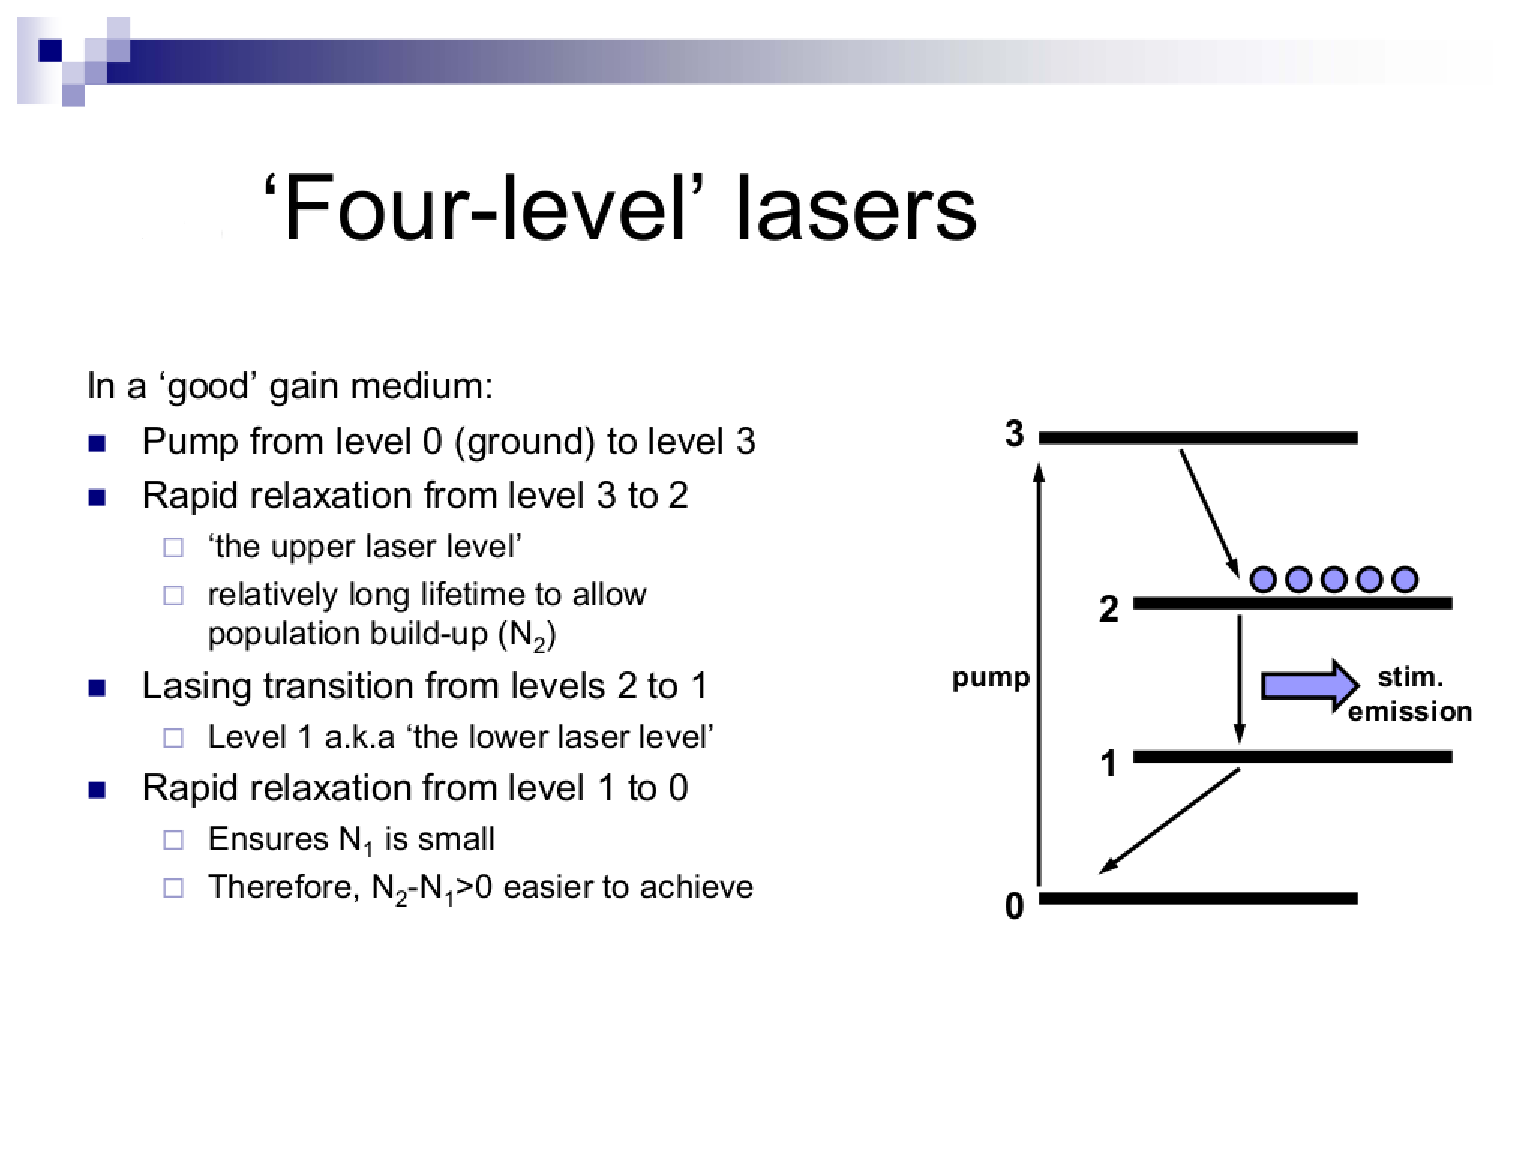
\includegraphics[scale=0.5]{laser3.eps}
\end{figure}
Emitting spieces chosen of ten because they are good "4-level" systems, i.e.\\
level 0 -- ground level\\
level 1 -- lower laser level\\
level 2 -- upper laser level\\
level 3 -- "pumpoint"

Choose spieces with $\tau_{21} >> \tau{31}$, $\tau_{10} \Rightarrow N_2 >> N_1$ with populaion $N \sim N_2$.

Now rate equation
\begin{equation*}
\dot{N_2} = R - N(B_{21}\rho + A_{21})
\end{equation*}

At steady state,
\begin{equation*}
\dot{N_2} = 0
\end{equation*}
\begin{equation*}
N = N_{TH}
\end{equation*}
\begin{equation*}
\rho = \left(\frac{R}{N_{TH}} - A_{21}\right) \frac{1}{B_{21}} = \frac{1}{N_{TH} B_{21}} \left(R - \frac{N_{TH}}{\tau_{21}} \right)
\end{equation*}
but
\begin{equation*}
I = \rho c
\end{equation*}
and
\begin{equation*}
\frac{B_{21}}{c} = \frac{\sigma}{h \nu}
\end{equation*}
\begin{equation*}
I = \frac{h \nu}{N_{TH} \sigma} \left(R - \frac{N_{TH}}{\tau_{21}} \right)
\end{equation*}
\begin{equation*}
I = \eta (R - R_{TH})
\end{equation*}

Threshold rate
\begin{equation*}
R = \frac{N_{TH}}{\tau_{21}}
\end{equation*}
$\Rightarrow$ rate of spontaneous amount threshold. "Slope efficiency".
\begin{figure}[h!]
\centering
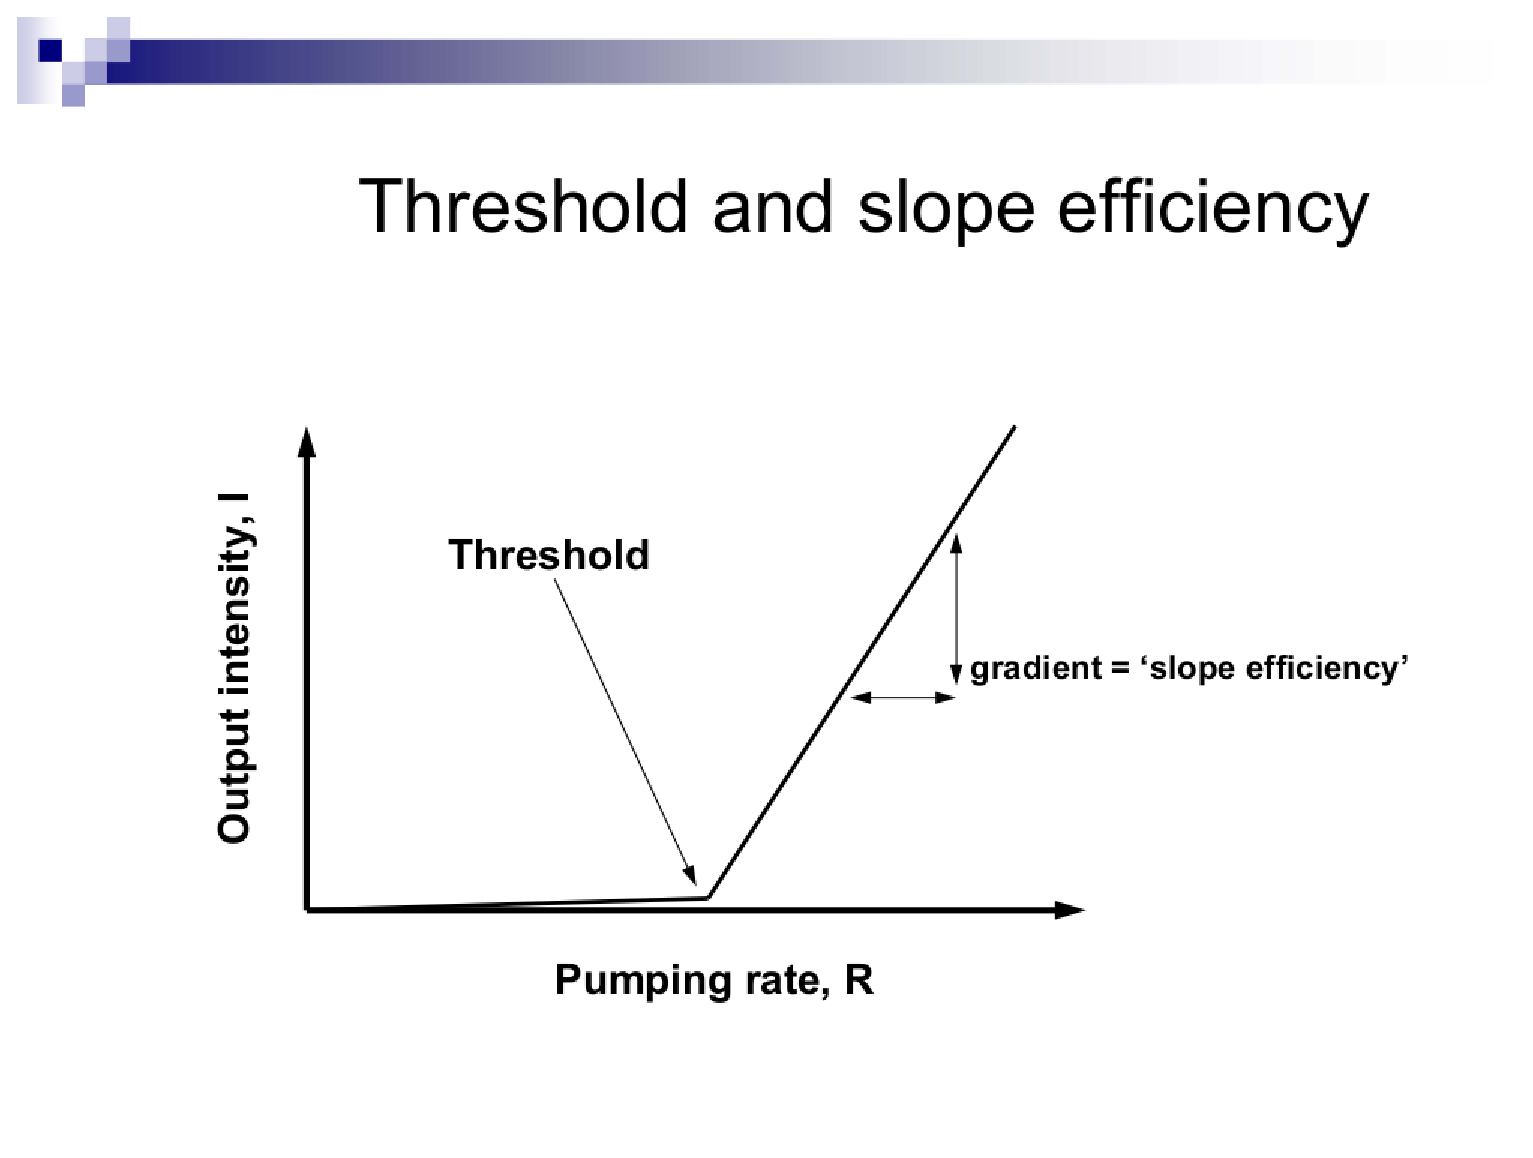
\includegraphics[scale=0.5]{laser4.eps}
\end{figure}
\begin{equation*}
\eta = \frac{h \nu}{N_{TH} \sigma}
\end{equation*}

\subsection{An example of gain medium Nd:YAG}
Yithrium Alliuminium Garnet ($Y_3CH_5O_{12}$) is: $Nd$ -- $1\%$ atoms with $Nd^{2+}$
\begin{figure}[h!]
\centering
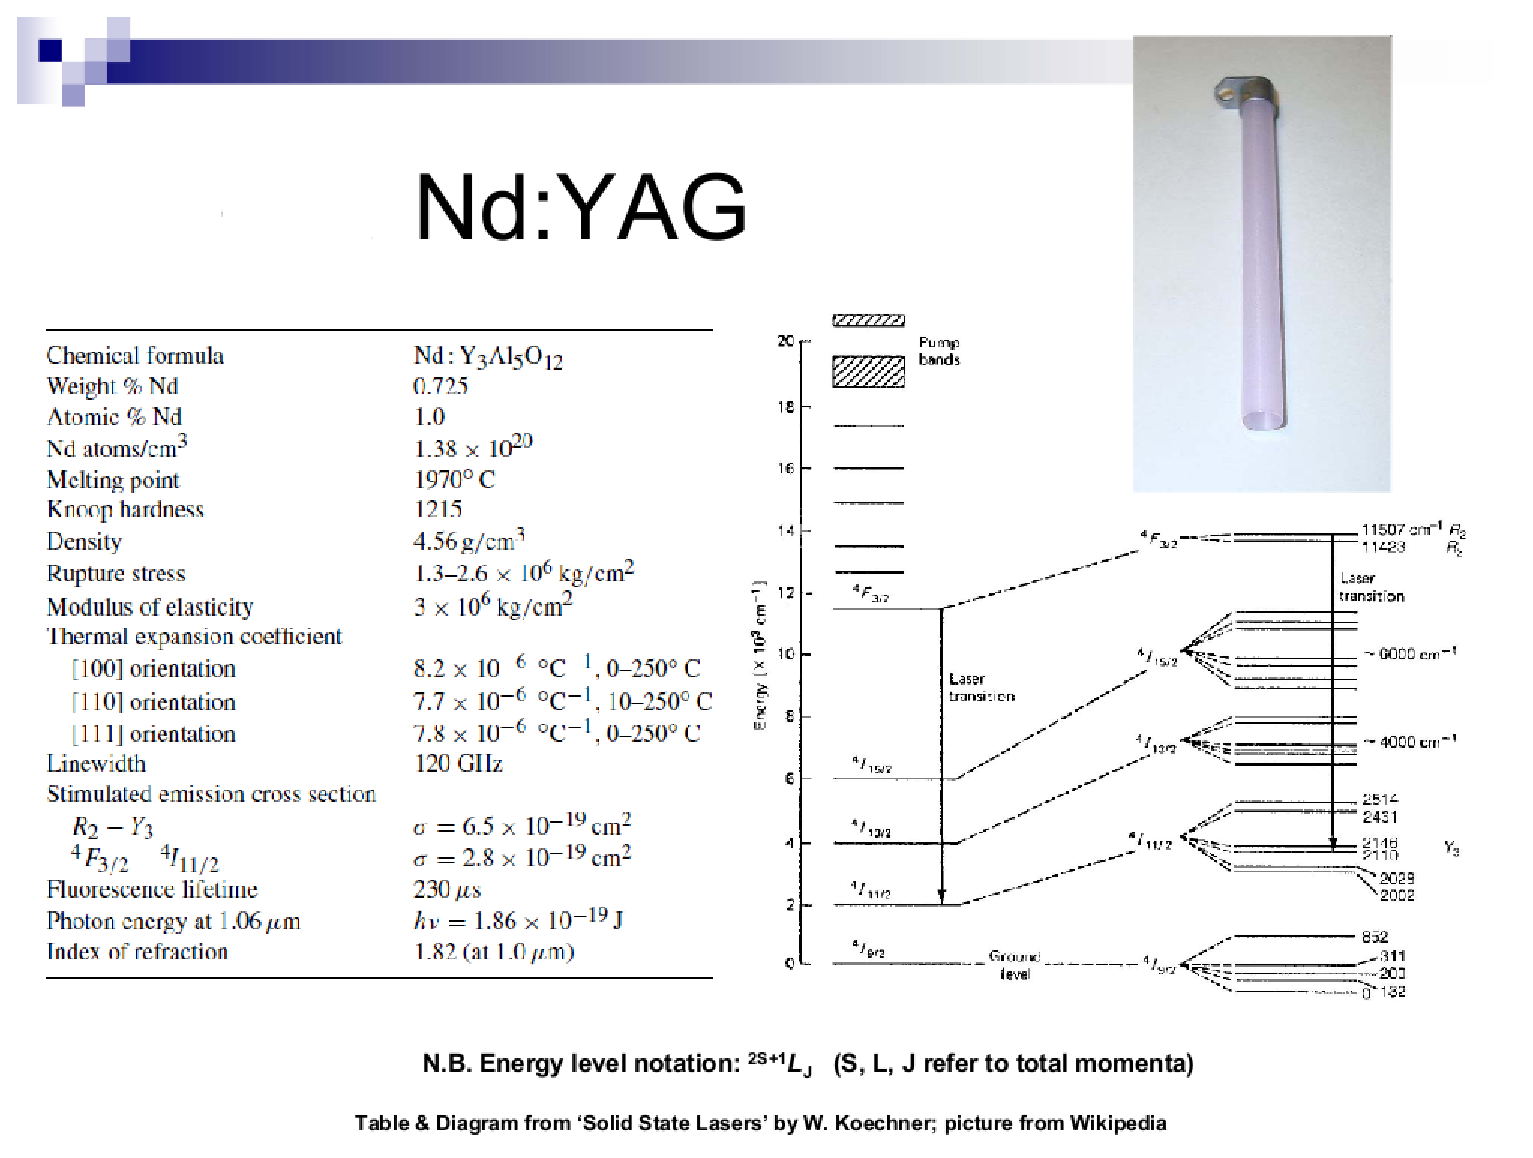
\includegraphics[scale=0.5]{laser5.eps}
\end{figure}
\begin{itemize}
\item[-] added as in impurity during crystal growth;
\item[-] $Nd^{2+}$ replaces $Y^{3+}$ lattice.
\end{itemize}


\end{document}